%=======================================================================
% slide.tex
%
% Session 3, "AI Tools: Introduction to Claude Code"
% Yale Master's in Asset Management (MAM) Orientation BootCamp
% Xugan Chen, Yale School of Management
%
% BUILD
% -----
%   latexmk -pdf slide.tex          (preferred; resolves refs in one go)
%   pdflatex slide.tex              (run twice)
%
% Build with pdflatex, NOT xelatex or lualatex: the preamble uses
% fontenc[T1] + inputenc[utf8], which is a pdflatex setup.
%
% Any frame containing a prompt/pycode/shellout block must be declared
% \begin{frame}[fragile].  See the header of utils/setup_teaching.tex.
%
% LAYOUT
% ------
%   utils/setup_teaching.tex  THE WHOLE PREAMBLE.  Theme, colours,
%                             macros, code blocks, frame furniture.
%                             The only file to edit for styling.
%   sections/*.tex            one file per block of the session.  Each
%                             is a plain sequence of frames with no
%                             preamble of its own.
%   figures/                  screenshots and plots (\graphicspath below)
%
% To reorder or drop a block, comment out its \input line.  Nothing in
% sections/ depends on anything else in sections/.
%
%=======================================================================

\documentclass[11pt,aspectratio=169]{beamer}

%=======================================================================
% setup_teaching.tex -- the entire preamble for this deck.
%
% Session 3, "AI Tools: Introduction to Claude Code"
% Yale MAM Orientation BootCamp
%
% slide.tex inputs this file and nothing else. Everything the deck needs
% is here: theme, colours, text macros, code blocks, frame furniture.
%
% Build with pdflatex. fontenc[T1] + inputenc[utf8] is a pdflatex setup;
% xelatex and lualatex want fontspec instead.
%
% THE ONE TRAP
% ------------
% Any frame containing a prompt / pycode / shellout block MUST be
% declared
%
%     \begin{frame}[fragile]{Title}
%
% Without [fragile], beamer scans the frame body before listings can
% claim it, the \end{...} is never seen, and the run dies pages later
% with "Text dropped after begin of listing" followed by an emergency
% stop pointing at the end of the file rather than at your frame. This
% is the most likely way to break this deck.
%
% House style: ASCII punctuation. Write "--" for a dash and "'" for an
% apostrophe. Both render identically to their Unicode forms and survive
% being copied into a terminal. UTF-8 compiles fine, so an accented
% author name is not a problem.
%=======================================================================


%=======================================================================
% 1. Theme and packages
%=======================================================================
% Add a package here only when a frame needs it, with a comment saying
% which one. The list is short on purpose.

\usetheme{Szeged}
\usecolortheme{seahorse}

\usepackage[T1]{fontenc}
\usepackage[utf8]{inputenc}
\usepackage[english]{babel}

\usepackage{lmodern}          % scalable Latin Modern. Supplies the
                              % monospace face the listings blocks use:
                              % lato has no mono, and without lmodern
                              % the code blocks fall back to bitmap cmtt
\usepackage[default]{lato}    % text font, matching the research decks

\usepackage{xcolor}
\usepackage{graphicx}
\usepackage{booktabs}         % \toprule \midrule \bottomrule
\usepackage{colortbl}         % \rowcolor, to tint one row of a table
\usepackage{amsmath}
\usepackage{listings}
\usepackage{tikz}             % box-and-arrow diagrams; see \flowbox below
\usetikzlibrary{arrows.meta,positioning}
\usepackage{hyperref}
\usepackage{pgfpages}         % required by \setbeameroption below

% Speaker notes. This deck ships with notes hidden. To write them, put
% \note{...} after a frame and switch the option. Presenting from a
% laptop with an external screen wants the third form.
\setbeameroption{hide notes}
%\setbeameroption{show only notes}
%\setbeameroption{show notes on second screen=right}


%=======================================================================
% 2. Colours and text macros
%=======================================================================

\definecolor{yaleblue}{HTML}{00356b}
\definecolor{ylb}{HTML}{286dc0}
\definecolor{yo}{HTML}{bd5319}
\definecolor{lightgray}{HTML}{d3d3d3}

% Emphasis, in descending order of how much attention it claims:
%   \ybb  Yale blue bold  -- main emphasis. The finding on a slide.
%   \ylbb light blue bold -- secondary emphasis.
%   \yob  orange bold     -- warnings, and the thing that broke.
\newcommand\yb[1]{{\color{yaleblue} #1}}
\newcommand\ybb[1]{{\color{yaleblue} \textbf{#1}}}
\newcommand\ylb[1]{{\color{ylb} #1}}
\newcommand\ylbb[1]{{\color{ylb} \textbf{#1}}}
\newcommand\yo[1]{{\color{yo} #1}}
\newcommand\yob[1]{{\color{yo} \textbf{#1}}}

% \blue, \red and \green are left undefined on purpose. The MAM course
% decks in slides/misc define those names with different colours, so a
% frame copied in from one of them fails loudly with "Undefined control
% sequence" rather than quietly drawing the wrong colour. Use the Yale
% macros above.


%=======================================================================
% 3. Beamer appearance
%=======================================================================

\setbeamercolor{structure}{fg=white}
\setbeamercolor{title}{fg=yaleblue,bg=white}
\setbeamercolor{frametitle}{fg=yaleblue,bg=white}
\setbeamercolor{button}{bg=yaleblue!10,fg=yaleblue}

\setbeamerfont{frametitle}{size=\fontsize{14pt}{12pt}}
\setbeamertemplate{frametitle}[default][center]
\addtobeamertemplate{frametitle}{\vspace*{0cm}}{\vspace*{-0.5cm}}

\setbeamertemplate{itemize items}[default]
\setbeamercolor{itemize item}{fg=ylb,bg=white}
\setbeamercolor{itemize subitem}{fg=ylb,bg=white}
\setbeamercolor{itemize subsubitem}{fg=ylb,bg=white}
\setbeamertemplate{itemize subitem}[triangle]
\setbeamertemplate{itemize subsubitem}[triangle]

\setbeamertemplate{enumerate items}[default]
\setbeamercolor{enumerate item}{fg=ylb,bg=white}
\setbeamercolor{enumerate subitem}{fg=ylb,bg=white}

\setbeamertemplate{navigation symbols}{}
\setbeamersize{text margin left=0.5cm,text margin right=0.5cm}

% Tighter display maths.
\makeatletter
\g@addto@macro\normalsize{
  \setlength\abovedisplayskip{5pt}
  \setlength\belowdisplayskip{5pt}
  \setlength\abovedisplayshortskip{5pt}
  \setlength\belowdisplayshortskip{5pt}
}
\makeatother

\setbeamertemplate{section page}{
  \begin{centering}
  \fontsize{20}{16} {\color{yaleblue} \textsc{\insertsection}} \par
  \end{centering}
}

%----------------------------------------------------------------------
% 3a. No navigation bar across the top
%----------------------------------------------------------------------
% Szeged puts a miniature table of contents in the headline: a row of
% section names with a progress dot per frame. It is blanked here. Over
% 86 frames the dots compress to unreadable pinheads, the bar costs
% about a centimetre of vertical space on every slide, and none of it
% reads from the back of a lecture hall.
%
% To put it back, delete this one line.
\setbeamertemplate{headline}{}

% The footline carries the position information instead: short title on
% the left, institute and then the frame number on the right.
% Keep the frame number if you restyle this -- it is what lets someone
% in row 12 ask about "slide 47".
%
% The left half prints \insertshorttitle (the bracketed argument of
% \title) and the right half \insertshortinstitute (the bracketed
% argument of \institute), so both are set in slide.tex, not here.
\setbeamercolor{footline}{fg=yaleblue}
\setbeamerfont{footline}{size=\fontsize{6.5pt}{8pt}}
\setbeamertemplate{footline}{%
  \hbox{%
    \begin{beamercolorbox}[wd=.55\paperwidth,ht=2.4ex,dp=1.2ex,leftskip=.3cm]%
      {footline}\usebeamerfont{footline}\insertshorttitle
    \end{beamercolorbox}%
    \begin{beamercolorbox}[wd=.45\paperwidth,ht=2.4ex,dp=1.2ex,rightskip=.3cm]%
      {footline}\usebeamerfont{footline}\hfill
      \insertshortinstitute{} \quad \insertframenumber{} / \inserttotalframenumber
    \end{beamercolorbox}%
  }%
  \vskip0pt%
}


%=======================================================================
% 4. Code, prompts and terminal output
%=======================================================================
% White monospace on a cobalt block. Remember [fragile] on any frame
% that uses these; see the file header.

\definecolor{cobalt}{RGB}{0, 34, 64}
\definecolor{bluecomments}{RGB}{0, 103, 231}
\definecolor{colnum}{RGB}{251, 94, 133}
\definecolor{stringgreen}{RGB}{35, 185, 23}

% LST1: the default. "language=" is empty on purpose. This deck shows
% Python, shell and plain English prompts in the same style of block,
% and keyword highlighting applied to an English sentence looks like a
% rendering bug.
\lstdefinestyle{LST1}{
    language=,
    basicstyle=\scriptsize\ttfamily\color{white},
    commentstyle=\color{bluecomments},
    stringstyle=\color{stringgreen},
    numberstyle=\color{colnum},
    literate={~}{$\sim$}{1},
    backgroundcolor=\color{cobalt},
    showspaces=false,
    showstringspaces=false,
    linewidth=\linewidth,
    breaklines=true,
    breakatwhitespace=true,
    columns=fullflexible,
    keepspaces=true,
    escapeinside={(*@}{@*)}
}

% LST_fn: the same block one size up, for a short prompt that is the
% entire point of its slide and must read from the back row.
\lstdefinestyle{LST_fn}{
    language=,
    basicstyle=\footnotesize\ttfamily\color{white},
    commentstyle=\color{bluecomments},
    stringstyle=\color{stringgreen},
    numberstyle=\color{colnum},
    literate={~}{$\sim$}{1},
    backgroundcolor=\color{cobalt},
    showspaces=false,
    showstringspaces=false,
    linewidth=\linewidth,
    breaklines=true,
    breakatwhitespace=true,
    columns=fullflexible,
    keepspaces=true,
    escapeinside={(*@}{@*)}
}

% LSTpy: Python, for the few slides showing real source.
\lstdefinestyle{LSTpy}{
    language=Python,
    basicstyle=\scriptsize\ttfamily\color{white},
    keywordstyle=\color{ylb}\bfseries,
    commentstyle=\color{bluecomments},
    stringstyle=\color{stringgreen},
    backgroundcolor=\color{cobalt},
    showspaces=false,
    showstringspaces=false,
    linewidth=\linewidth,
    breaklines=true,
    breakatwhitespace=true,
    columns=fullflexible,
    keepspaces=true,
    escapeinside={(*@}{@*)}
}

\lstset{style=LST1}

% \begin{prompt} ... \end{prompt}
% A prompt as it was actually run. Every prompt in this deck is quoted
% verbatim; the same text is in ../project/prompts/. Do not paraphrase
% one on a slide: the point of showing it is that those exact words did
% the work.
\lstnewenvironment{prompt}[1][]
  {\lstset{style=LST_fn,#1}}
  {}

% \begin{pycode}   -- Python source
% \begin{shellout} -- terminal or agent output
%
% Named pycode and shellout because beamer already claims the names
% "code" and "output"; \lstnewenvironment refuses to clobber an
% existing environment.
\lstnewenvironment{pycode}[1][]
  {\lstset{style=LSTpy,#1}}
  {}
\lstnewenvironment{shellout}[1][]
  {\lstset{style=LST1,#1}}
  {}


%=======================================================================
% 5. Frame furniture
%=======================================================================

% Looser lists. Prefer wideitemize on lecture frames; beamer's default
% spacing packs bullets too tightly to scan from a distance.
\newenvironment{wideitemize}{\itemize\addtolength{\itemsep}{8pt}}{\enditemize}
\newenvironment{wideenumerate}{\enumerate\addtolength{\itemsep}{8pt}}{\endenumerate}

% A part divider: nothing but the part title, large, Yale blue, centred
% on a white slide.  Used once at the top of each of the four parts so
% the room always knows where it is in three hours.
%
% The body is centred both ways, so write only the title inside:
%
%     \begin{transitionframe}
%     Part 2: Building a private credit dataset
%     \end{transitionframe}
%
% Sizing is set here (\Large, bold) -- do not re-size inside the body,
% or the four dividers stop matching each other.
\newenvironment{transitionframe}{
  \setbeamercolor{background canvas}{bg=white}
  \setbeamercolor{normal text}{fg=yaleblue}
  \usebeamercolor[fg]{normal text}
  \centering
  \begin{frame}[plain]
  \vfill
  \leftskip=1.2cm \rightskip=1.2cm \parindent=0pt
  \centering
  \huge\bfseries}{
  \par\vfill
  \end{frame}
}

% \takeaway{...} -- the one sentence a slide exists to deliver, as a
% tinted full-width band. At most one per frame, and deliberately not on
% every frame: if every slide has one, none of them land.
\newcommand{\takeaway}[1]{%
  \vspace{0.3em}%
  \begin{beamercolorbox}[wd=\textwidth,sep=6pt,rounded=true]{button}%
  \small #1%
  \end{beamercolorbox}%
}

% \source{...} -- provenance line at the foot of the frame, deliberately
% quiet. Every frame stating a measured number carries one, naming the
% memo the number came from. This is not decoration: the deck argues
% that unsourced numbers are the problem it is teaching about.
\newcommand{\source}[1]{%
  \vfill{\scriptsize\color{gray} #1\par}}

% \capture{height fraction}{what to shoot} -- a dashed grey box standing in
% for a screenshot that has not been taken yet.  It renders in the PDF on
% purpose, so a missing capture is visible when the deck is reviewed rather
% than silently absent.  To fill it, replace the whole \capture call with
%     \begin{center}\includegraphics[width=...]{file}\end{center}
% Nothing else on the frame needs to change.
\newcommand{\capture}[2]{%
  \begin{center}
  \begin{tikzpicture}
    \node[draw=lightgray, dashed, line width=0.8pt, rounded corners=3pt,
          fill=lightgray!12, text=gray, align=center, font=\small,
          text width=0.78\textwidth, minimum height=#1\textheight]
         {capture needed: #2};
  \end{tikzpicture}
  \end{center}}

%----------------------------------------------------------------------
% 5a. Box-and-arrow diagrams
%----------------------------------------------------------------------
% Three tikz node styles for flow diagrams:
%   flowbox       a neutral step, or one the tool takes
%   flowbox_us   a step you take -- filled Yale blue
%   flowbox_warn  the thing that went wrong -- orange
% The deck uses the colour difference to carry an argument, so pick the
% style by meaning, not by position. Draw arrows with [flowarrow].
%
%   \begin{tikzpicture}[node distance=4mm]
%     \node[flowbox_us] (a) {instruct};
%     \node[flowbox, right=of a] (b) {it acts};
%     \draw[flowarrow] (a) -- (b);
%   \end{tikzpicture}
%
% Box width is fixed so a row of them reads as one strip. Change
% text width= here, not per diagram.
\tikzset{
  flowbox/.style={
    draw=yaleblue!40, line width=0.6pt, rounded corners=2pt,
    fill=yaleblue!5, text=yaleblue!80!black,
    align=center, font=\small,
    text width=2.55cm, inner sep=5pt, minimum height=1.15cm},
  flowbox_us/.style={
    flowbox, fill=yaleblue, draw=yaleblue, text=white, font=\small\bfseries},
  flowbox_warn/.style={
    flowbox, fill=yo!8, draw=yo!50, text=yo},
  flowarrow/.style={
    -{Stealth[length=2.4mm]}, line width=0.9pt, color=yaleblue!70},
  flowlabel/.style={font=\scriptsize, text=yo, align=center},
}

\newcommand{\tabfont}{\fontsize{9}{10}\selectfont}  % shrink a wide table
\newcommand{\file}[1]{{\ttfamily\small #1}}          % file and field names
\newcommand{\vs}{\vspace{0.5em}}


\graphicspath{{./figures/}}

%----- TITLE PAGE ------------------------------------------------------
\title[AI Tools: Introduction to Claude Code]{\Large AI Tools: Introduction to Claude Code}
\author[Chen]{\normalsize \textbf{Xugan Chen}}
% The bracketed forms below are what the footline prints: \insertshorttitle
% on the left, \insertshortinstitute on the right. Keep them short.
\institute[Xugan Chen (Yale)]{\normalsize \textit{Yale School of Management} \bigskip}
\date{\small MAM Orientation BootCamp \\ August 27, 2026}

\begin{document}

\linespread{1.4}

\begin{frame}[plain]
\titlepage
\end{frame}

%=======================================================================
%                              PART 1
%=======================================================================
% Part 1: Introduction. 14 frames, lecture, session 0:00-0:20.
\section{Introduction}\subsection{}

% Instructor intro. Keep it to a minute.
\begin{frame}{About me}
\begin{wideitemize}
  \item \ybb{Xugan Chen} -- PhD candidate, Financial Economics, Yale SOM.
        At Yale since 2020 (predoc 2020--2022, PhD since 2022).
  \item \ybb{TA for:} Entrepreneurial Finance; Venture Capital and Private Equity;
        Statistical Foundations; Behavioral Finance.
  \item \ybb{Research:} innovation; AI in finance and economics; corporate
        finance; entrepreneurial finance.
\end{wideitemize}
\vs
\begin{center}
\yob{Feedback is welcome -- now, or any time after today.}
\end{center}
\end{frame}

% Poll 1: who has used what.
\begin{frame}{Getting to know you}
Show of hands. Which side of each pair are you here for?
\vs
\begin{center}
\begin{tabular}{rcl}
\ybb{Public markets}      & vs & \ybb{Private markets} \\[0.6em]
\ybb{Industry}            & vs & \ybb{Academia} \\[0.6em]
\ybb{Quant research}      & vs & \ybb{Fundamental research} \\[0.6em]
\ybb{Equities}            & vs & \ybb{Other asset classes} \\
\end{tabular}
\end{center}
\vs
Today's task sits in \yob{private markets}, and the workflow is the same
whichever side you raised your hand on.
\end{frame}

% Poll 2: the tool ladder. Figure adapted from Kyle Jensen.
\begin{frame}{Getting to know you: How do you use AI tools?}
\vs
\begin{center}
\tabfont
\begin{tabular}{ll}
\toprule
\textbf{Tool} & \textbf{What you actually do} \\
\midrule
Browser chat & Copy code out, paste it in, run it, paste the error back \\
Agentic IDE (Cursor)              & Tell it what to do; it edits files inside the editor \\
\rowcolor{yaleblue!10} \ybb{Terminal agent} (Claude Code, Codex) & \ybb{Full environment}: reads, writes, runs commands, plans \\
Terminal agent plus MCP tools            & Wire it to databases, APIs, other services \\
Agent in a container              & One instruction, and leave alone \\
\bottomrule
\end{tabular}
\end{center}
\vs
\ybb{Today is the terminal agent}, with one look at agents in a container at the end.
Agent in a container is not better; it is more setup.
\source{Ladder adapted from Kyle Jensen.}
\end{frame}

% What the tool was a year ago: chat, copy, paste.
\begin{frame}{Working with AI, one year ago}
\begin{wideitemize}
  \item A \yob{chat window}. We describe the problem in prose, it hands back a
        snippet, we paste the snippet.
  \item It could not see our data, our files, or our errors. We were the
        clipboard between the model and the project.
  \item The code was \yob{roughly right and often not runnable}, which meant we
        still had to be the one who ran it.
\end{wideitemize}
\vs
\begin{center}
That is the version most people still have in mind.
\end{center}
\end{frame}

% What it is now: it acts inside your project.
\begin{frame}{Working with AI, now: it acts in our project}
An agent that lives in our terminal, inside our project directory.
\vs
\begin{wideitemize}
  \item \ybb{Reads and writes files} in the repo -- our data, our code, our notes.
  \item \ybb{Runs commands} -- installs packages, executes scripts, reads the errors.
  \item \ybb{Iterates} -- sees its own output fail and tries again, without us retyping.
\end{wideitemize}
\takeaway{It does not hand us a snippet to paste. It acts in the project and \ybb{lives with the consequences.}}
\end{frame}

% The instruct-and-review loop, as a diagram.
\begin{frame}{The loop is easy. Instruct and review is the job.}
\vs
\begin{center}
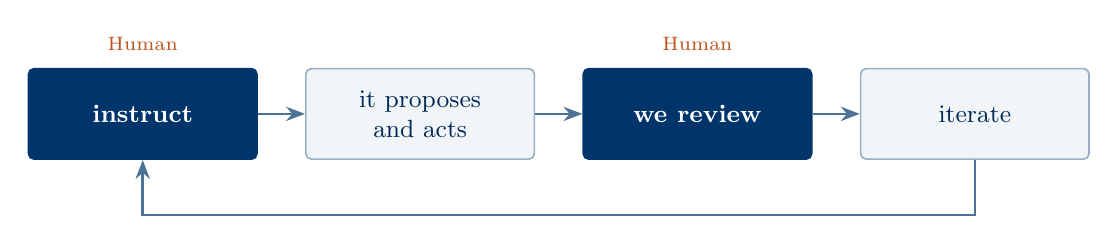
\begin{tikzpicture}[node distance=6mm]
  \node[flowbox_us]                (a) {instruct};
  \node[flowbox, right=of a]        (b) {it proposes\\and acts};
  \node[flowbox_us, right=of b]    (c) {we review};
  \node[flowbox, right=of c]        (d) {iterate};
  \draw[flowarrow] (a) -- (b);
  \draw[flowarrow] (b) -- (c);
  \draw[flowarrow] (c) -- (d);
  \draw[flowarrow] (d.south) -- ++(0,-0.7) -| (a.south);
  \node[flowlabel, above=1mm of a] {Human};
  \node[flowlabel, above=1mm of c] {Human};
\end{tikzpicture}
\end{center}
\vs
\begin{wideitemize}
  \item The two boxes with our names on them are \yob{the entire job}.
  \item Everything we add today -- planning, verification, generalization --
        makes the instruction sharper, or makes review possible on output
        that is \ybb{too large to read}.
\end{wideitemize}
\takeaway{For example, today we will sign off on a dataset of 37,197 rows without reading one of them.}
\end{frame}

% Why review is the hard half: it checks its own work.
\begin{frame}{Why reviewing is hard: it checks its own work}
\begin{wideitemize}
  \item Ask it to build a dataset and you usually get a check you did not ask
        for: \ylb{``I reconciled the total to the reported figure -- it matches.''}
  \item That is genuinely useful. It is also the trap, because \ybb{a check looks
        at one thing}, and the agent decided which thing.
\end{wideitemize}
\vs
\begin{center}
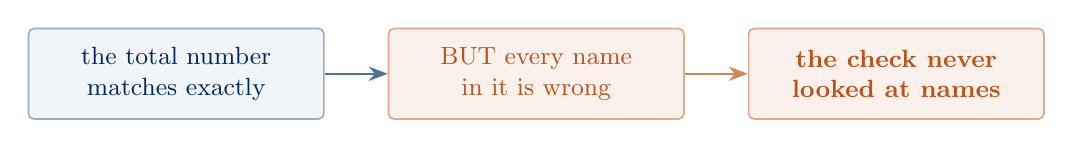
\begin{tikzpicture}[node distance=8mm]
  \node[flowbox, text width=3.4cm]                    (t) {the total number\\matches exactly};
  \node[flowbox_warn, right=of t, text width=3.4cm]   (n) {BUT every name\\in it is wrong};
  \node[flowbox_warn, right=of n, text width=3.4cm,
        font=\small\bfseries]                         (z) {the check never\\looked at names};
  \draw[flowarrow] (t) -- (n);
  \draw[flowarrow, color=yo!70] (n) -- (z);
\end{tikzpicture}
\end{center}
\vs
\takeaway{A check that passes tells you about \ybb{the part it looked at}. It says nothing about the rest.}
\begin{center}
\yob{We are going to meet this four times this afternoon}, and it looks different every time.
\end{center}
\end{frame}

% The objective for the afternoon.
\begin{frame}{Today's objective}
\begin{wideitemize}
  \item \yob{Not} a feature walkthrough -- the menu of options will have changed by October.
  \item \yob{Not} an intro to programming -- most of you can already code.
  \item \ybb{Is} \ybb{yours to build}, with the agent, on your own machine -- not a demo you watch.
  \item \ybb{Is} practice at \ybb{checking output you cannot read} -- tens of thousands of rows.
  \item \ybb{Is} practice at \ybb{patterns that move} to the rest of your work, not just to this task.
\end{wideitemize}
\takeaway{It is never \yob{``can it write the code''}. It is \yob{``how do I know this is right''} and \yob{``how do I scale it''}.}
\end{frame}

% The roadmap: four parts.
\begin{frame}{The roadmap}
\vs
\begin{center}
\tabfont
\renewcommand{\arraystretch}{1.4}
\begin{tabular}{p{0.60\textwidth}p{0.26\textwidth}}
\toprule
\textbf{Block} & \textbf{Mode} \\
\midrule
\textbf{1.} Introduction & lecture \\
\textbf{2.} Applied AM project: a private credit dataset from SEC filings & demo, then hands-on \\
\rowcolor{yaleblue!10} \quad \ybb{Break}, 10 minutes -- halfway through the project & \\
\quad \textit{...the project continues}: generalize, then analyse & hands-on \\
\textbf{3.} More useful concepts and tips & lecture \\
\textbf{4.} Advanced usage examples & demo \\
\bottomrule
\end{tabular}
\end{center}
\vs
\ybb{Half the session (in Part 2) is hands-on}. So have your
laptop out and Claude Code installed. Work on your own or with the person
next to you -- either is fine.
\end{frame}

% Install and access. 
\begin{frame}{Basic setup}
\begin{itemize}
  \item \ybb{Install} it, either way:
  \begin{itemize}
      \item With npm, if you have Node.js: \file{npm install -g @anthropic-ai/claude-code}
      \item Or the standalone installer, for Mac, Linux and Windows:
            \yb{\url{code.claude.com/docs}}
  \end{itemize}
  \item \ybb{Then} \file{cd} into a project folder and type \file{claude}. That is all.
\end{itemize}
\vspace{-0.2em}
\begin{center}
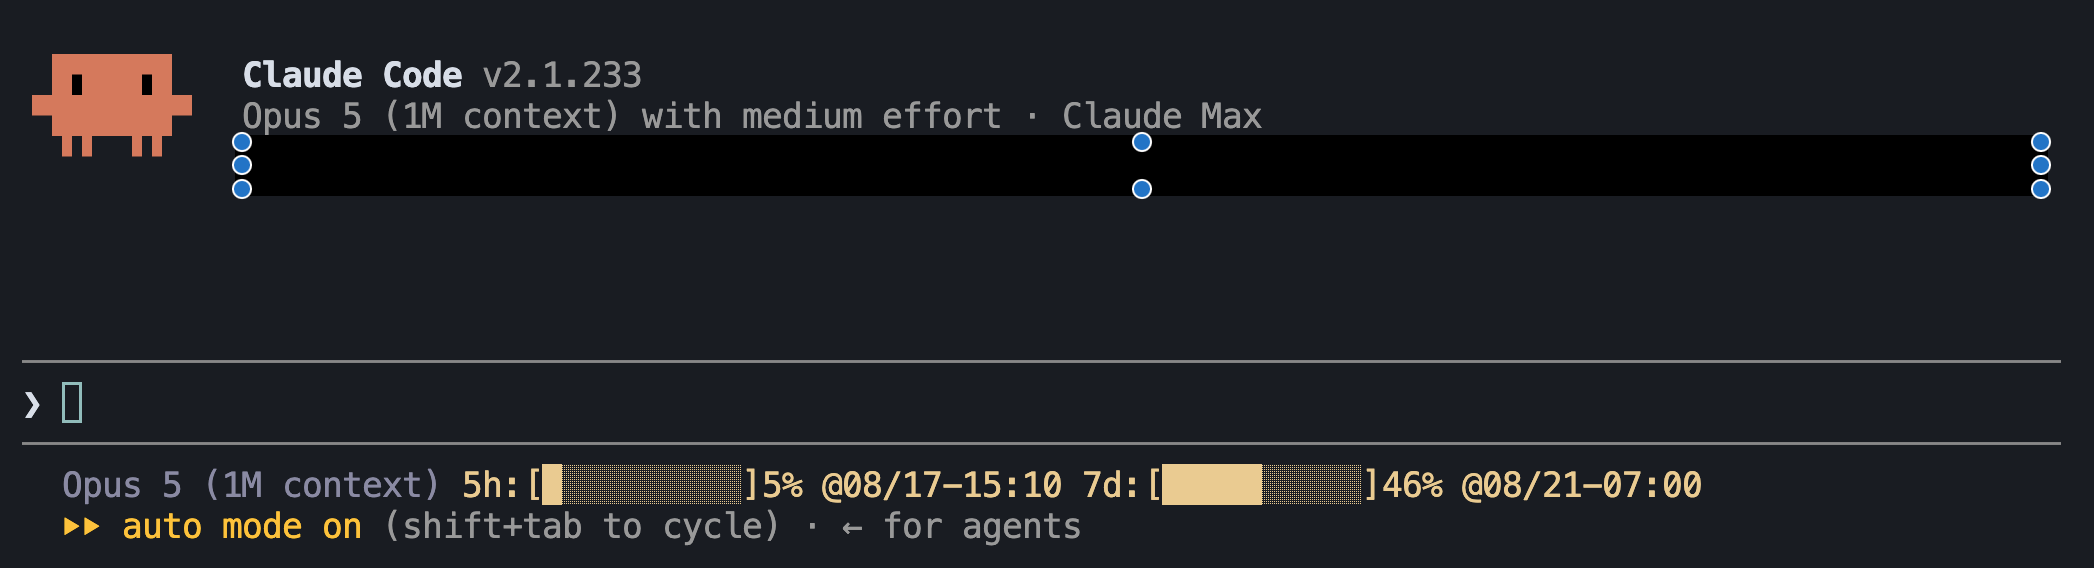
\includegraphics[width=0.86\textwidth]{claude_code.png}
\end{center}
\vspace{-0.3em}
{\small \yob{If your terminal doesn't look like this, fix it now}. The rest of
the session assumes a working install.}
\end{frame}

% Tokens: the unit everything is measured in.
\begin{frame}{Tokens: the unit everything is measured in}
\begin{wideitemize}
  \item \ybb{Tokens} are the pieces text is chopped into before the model sees it.
  \begin{itemize}
      \item The short sentence ``I love cats'' is broken into \ylbb{3 tokens} (I, love, cats).
      \item A longer word like ``unbreakable'' may be split into \ylbb{2 tokens} (un and breakable).
      \item Rule of thumb: in English, \ybb{1 token is about 4 characters, or 0.75 words}.
  \end{itemize}
  \item Claude Fable/Opus/Sonnet: a \ybb{1M-token context window}, roughly
        750,000 words.
  \item Later we will work on SEC filings -- \ylbb{one filing runs 10 to 25 MB of HTML}.
  \begin{itemize}
      \item At 25 MB that is roughly \yob{6 million tokens -- six full context windows}.
      \item \ybb{So nothing ever reads the whole document.} It gets searched, sliced, and read a slice at a time. You will watch that happen this afternoon.
  \end{itemize}
\end{wideitemize}
\end{frame}

% Context window: long sessions degrade, so plan for it.
\begin{frame}{Context window: Long sessions degrade, so plan for it.}
\vspace{-0.2em}
\begin{columns}[T]
\begin{column}{0.4\textwidth}
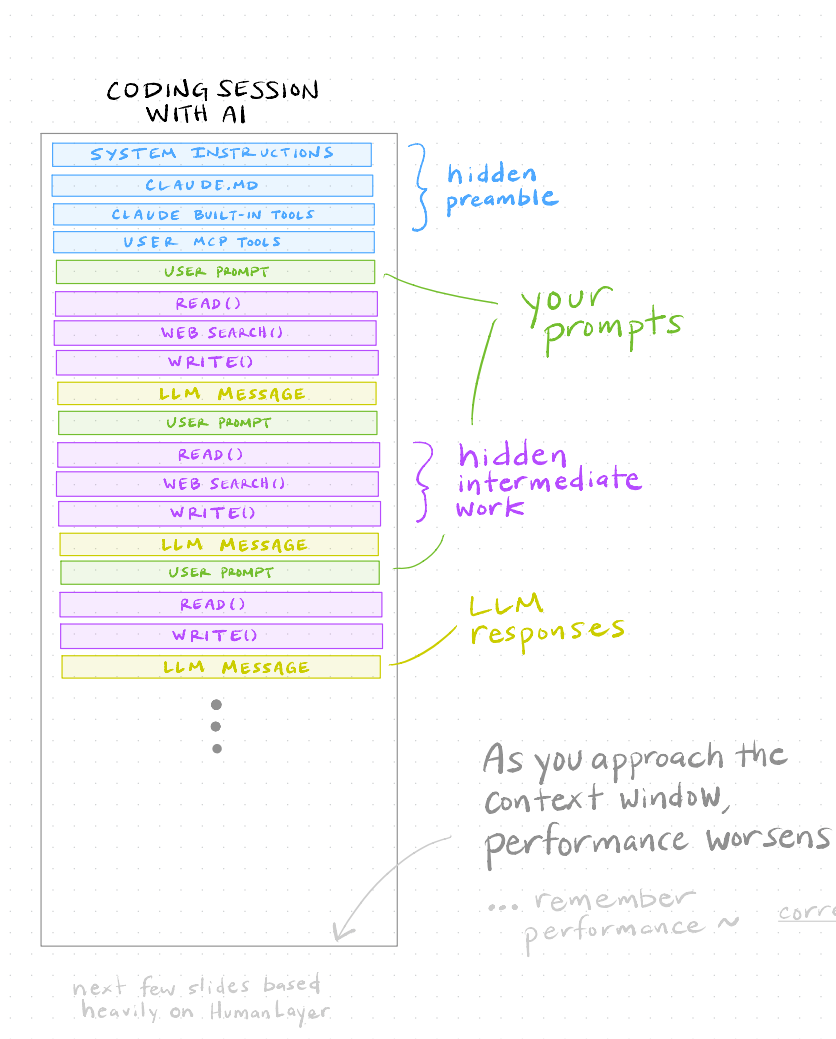
\includegraphics[width=1\textwidth]{context_window2.png}
\end{column}
\begin{column}{0.6\textwidth}
\vs
\begin{itemize}\small
  \item A ``chat'' is \ybb{one long document} passed back and forth: system
        prompt, tool definitions, thinking, tool calls, results. All of it
        counts against the window, and we only see the output.
  \item \ybb{Write state to files.} A decision that lives only in the
        conversation is gone. Files persist.
  \item \ybb{Work in chunks.} Five to ten turns with one objective, then start
        fresh. Your agent at turn 30 is noticeably worse than at turn 3.
  \item \ybb{Compact.} \file{/compact} summarizes, writes to files, and continues.
\end{itemize}
\end{column}
\end{columns}
\source{Source: A Series on Claude Code by Paul Goldsmith-Pinkham.}
\end{frame}

% Housekeeping and the break.
\begin{frame}{Housekeeping}
\begin{wideitemize}
  \item \ybb{No homework, no grading.} Nothing is submitted.
  \item \ybb{Everything ships:} every prompt as it was run, every plan -- and the failures.
  \item \yob{No code is provided} -- We will build everything with the agent.
\end{wideitemize}
\vs
\begin{center}
\yb{\url{github.com/xuganchen/BootCamp-Introduction-to-Claude-Code}}
\end{center}
\end{frame}


%=======================================================================
%                    PART 2: THE APPLIED AM PROJECT
%=======================================================================
% Part 2 opener: the applied AM project. Divider plus 3 frames, ~6 minutes.
\section{The Project}\subsection{}

% Part 2 divider.
\begin{transitionframe}
Part 2. Building a private credit dataset from raw SEC filings
\end{transitionframe}

% Motivation: why private credit, and why BDCs.
\begin{frame}{Why private credit, and why BDCs}
\begin{wideitemize}
  \item Private credit is the \ybb{fastest-growing corner of asset management}.
  \item \ybb{BDC filings are its only public window.} A BDC lends to middle-market borrowers and must disclose \yb{every position, every quarter}.
  \item \ybb{The filing grades your work.} The positions foot to the balance sheet, so you can check the agent against an audited number.
\end{wideitemize}
\takeaway{A real AM dataset, with a ground truth to check it against, free and public.}
\end{frame}

% The document itself. Figures measured on ARCC's 2026 Q2 10-Q.
\begin{frame}{Investment position data from raw SEC filings}
\begin{itemize}
  \item A position-by-position table of \ybb{every loan the fund holds}: borrower,
        industry, lien seniority, spread, maturity, cost, fair value.
  \item Filed quarterly inside the 10-K and 10-Q, back roughly two decades.
  \item Example -- ARCC's 2026 Q2 10-Q: \ybb{24.8 MB, 275 HTML tables, $\sim$6 million tokens}.
        \yob{You cannot paste this into a chat window.}
\end{itemize}
\vspace{-0.3em}
\begin{center}
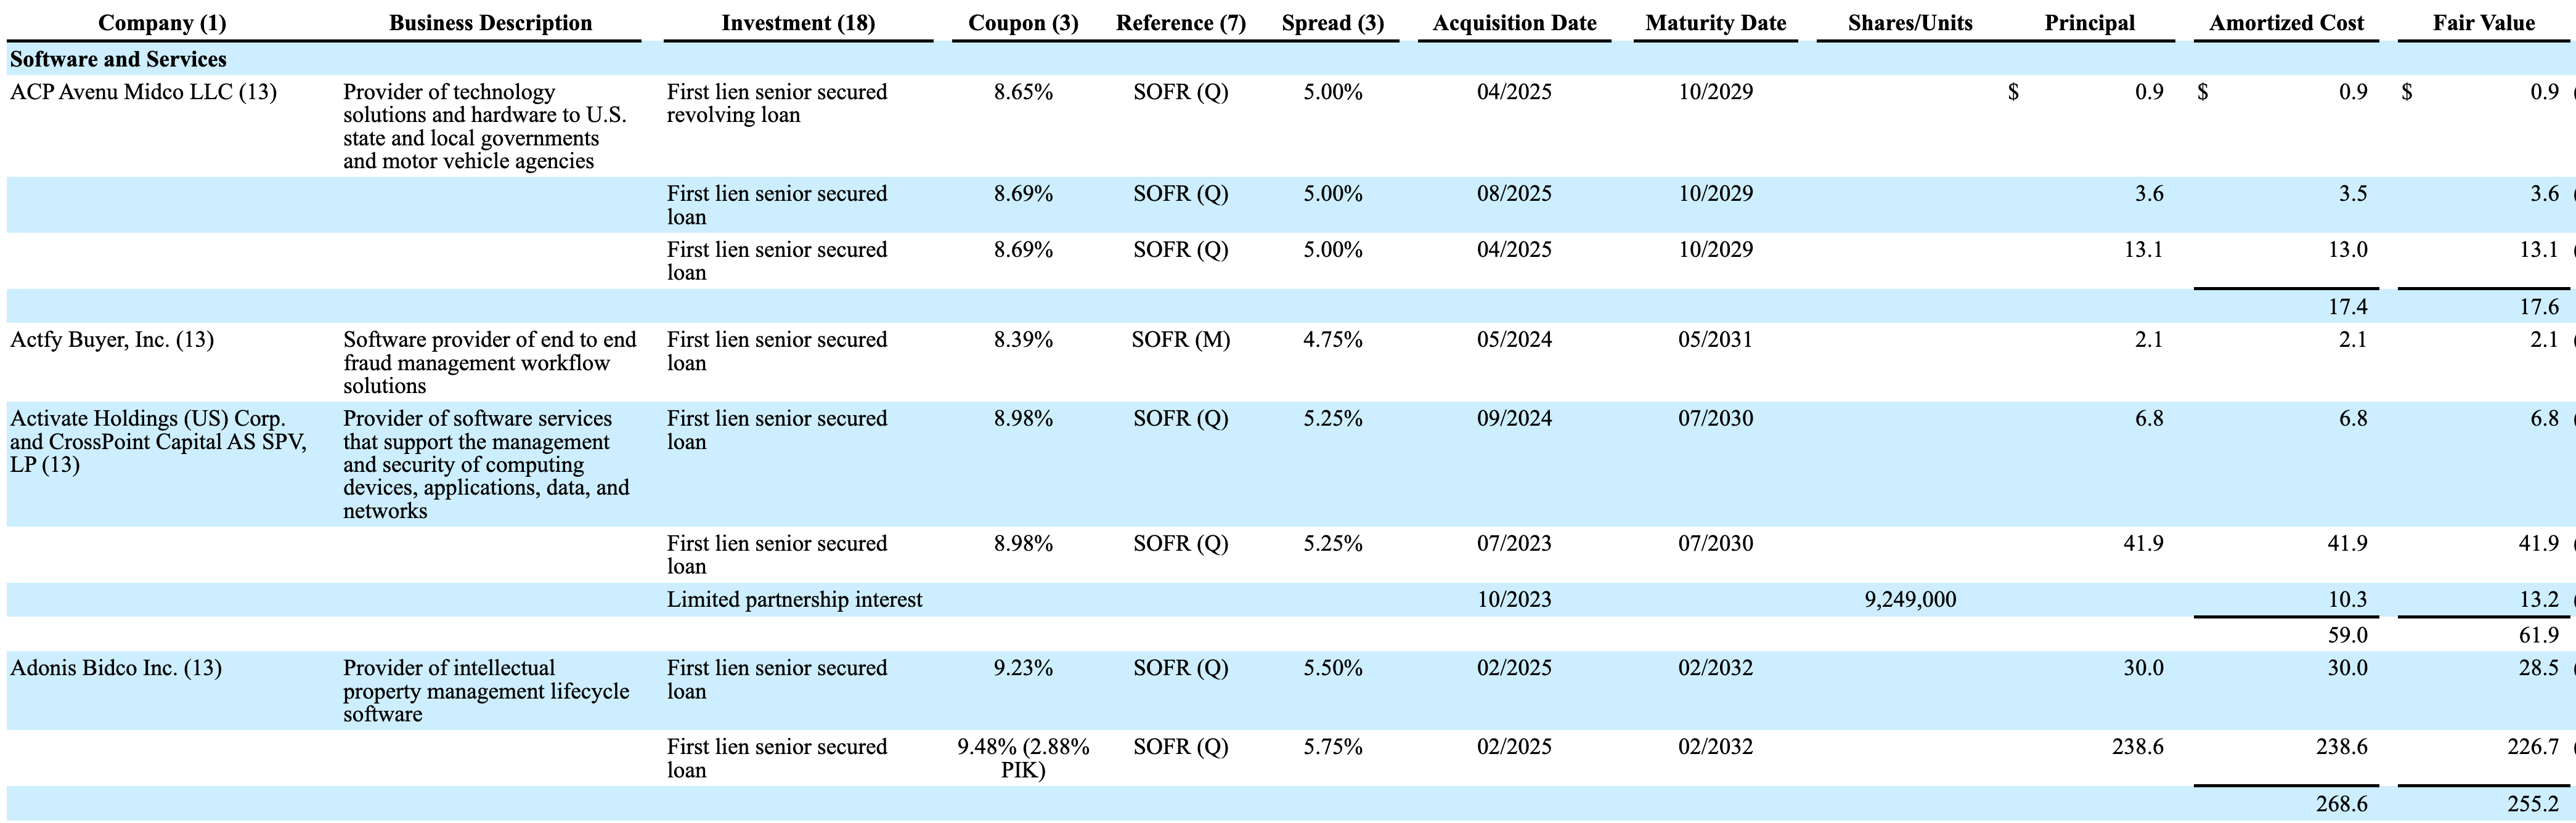
\includegraphics[width=0.9\textwidth]{ARCC_example.png}
\end{center}
\end{frame}

% What each student builds: the two panels, and the four steps.
\begin{frame}{Building a private credit dataset from SEC filings}

\begin{itemize}
  \item \ybb{Panel A -- BDC-quarter}
  \begin{itemize}
      \item One row per BDC per quarter: \yb{fund-level financial statements}.
      \item NAV, leverage, portfolio yield, portfolio size, non-accruals, etc.
  \end{itemize}
  \item \ybb{Panel B -- BDC-quarter-investment}
  \begin{itemize}
      \item One row per investment position per quarter: \yb{deal-level terms}.
      \item Borrower, loan type, seniority, spread, maturity, cost, fair value, etc.
  \end{itemize}
  \item \ybb{Pick your own BDC} (a large one is easiest), window
        \ybb{2023-01-01 to now}.
\end{itemize}

\begin{center}
\tabfont
\begin{tabular}{cll}
\toprule
Step & What we build & The concept it forces \\
\midrule
0 & Naive baseline: one prompt & A passing check is only as good as its \ybb{scope} \\
1 & Write a spec, then build & \ybb{Plan mode}, \ybb{sub-agents} for independent verification \\
2 & Generalize across quarters & \ybb{Skills}, and the tie-out as a test suite \\
3 & Analysis and report & Analysis as verification; \ybb{grounding} in your references \\
\bottomrule
\end{tabular}
\end{center}

\end{frame}

% Step 0: the naive baseline. 14 frames, DEMO not lab, session 0:20-0:35.
\section{Step 0. The naive baseline}\subsection{}

% Step 0 opener. Step table, this row tinted.
\begin{frame}{Step 0. The naive baseline}
\begin{center}
\tabfont
\begin{tabular}{cll}
\toprule
Step & What we build & The concept it forces \\
\midrule
\rowcolor{yo!10}\yob{0} & \yob{Naive baseline: one prompt} & \yob{A passing check is only as good as its scope} \\
1 & Write a spec, then build & \ybb{Plan mode}, \ybb{sub-agents} for independent verification \\
2 & Generalize across quarters & \ybb{Skills}, and the tie-out as a test suite \\
3 & Analysis and report & Analysis as verification; \ybb{grounding} in your references \\
\bottomrule
\end{tabular}
\end{center}
 
\vs
\begin{itemize}
    \item I will walk through my own output in detail; you do not need to type anything.
    \item It took $\sim$15 to 20 minutes to finish this one simple prompt.
    \item I experimented with three different models: Opus 5 at xhigh effort, Opus 5 at medium effort, and Sonnet 5 at medium effort.
\end{itemize}
\end{frame}

% The prompt, verbatim.
\begin{frame}[fragile]{Start with the laziest possible prompt}
\begin{prompt}
Find a large publicly traded BDC, download its most recent 10-Q from SEC EDGAR, and parse the financial statements and the schedule of investments into two structural tables I can analyze.
\end{prompt}
\vs
\begin{wideitemize}
  \item Not in it: a ticker, a schema, a file format, a variable list.
  \item Not in it: how to download or paste the filing.
  \item Not in it: any word about verifying anything.
\end{wideitemize}
\end{frame}

% It picked its own target and surveyed the filing before parsing it.
% MERGED 2026-08-19 (clock): was two frames, 'It picked its own target' and
% 'It reads the document before parsing it'.  Split them again if the block
% ever gets its time back; both screenshots are still here.
\begin{frame}{It picked its own target, and looked before it parsed}
\begin{columns}
\begin{column}{0.5\textwidth}
\begin{center}
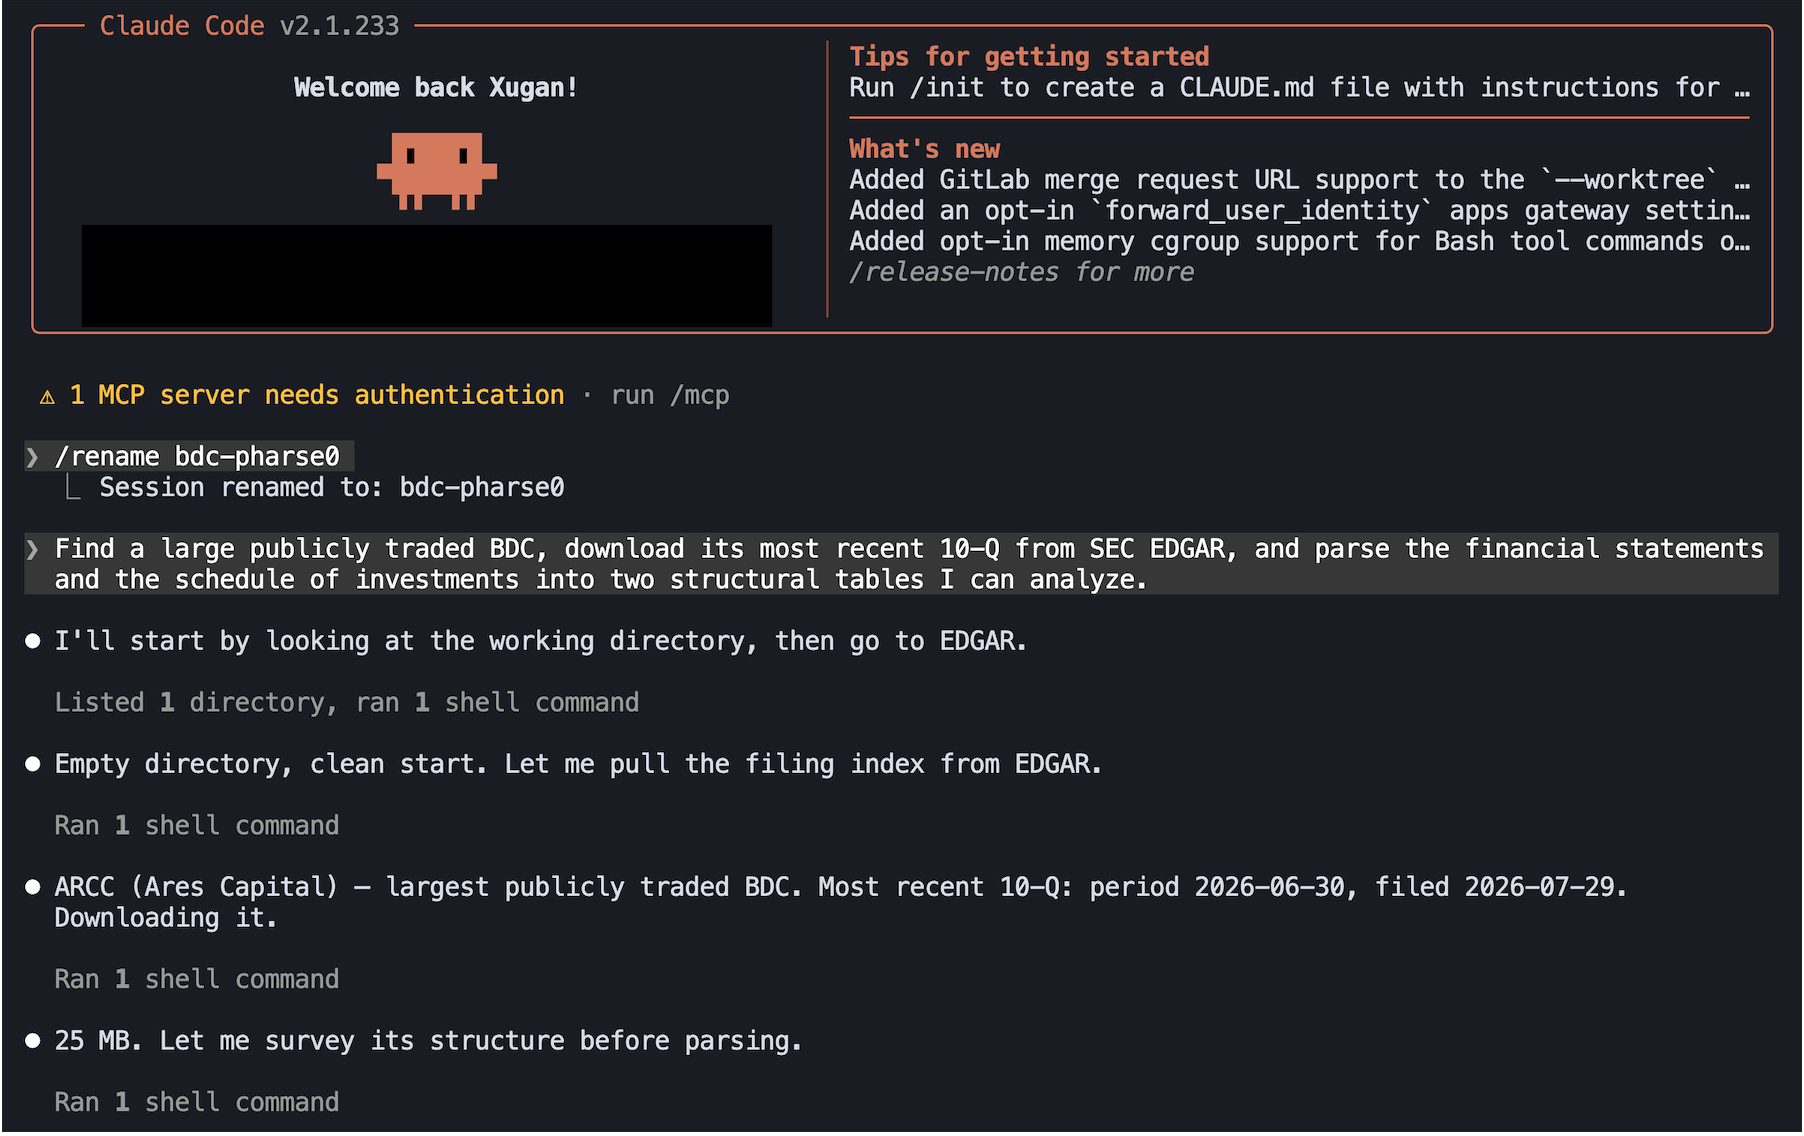
\includegraphics[width=0.9\textwidth]{bdc_design_pharse0-1.png}
\end{center}
\end{column}
\begin{column}{0.5\textwidth}
\begin{center}
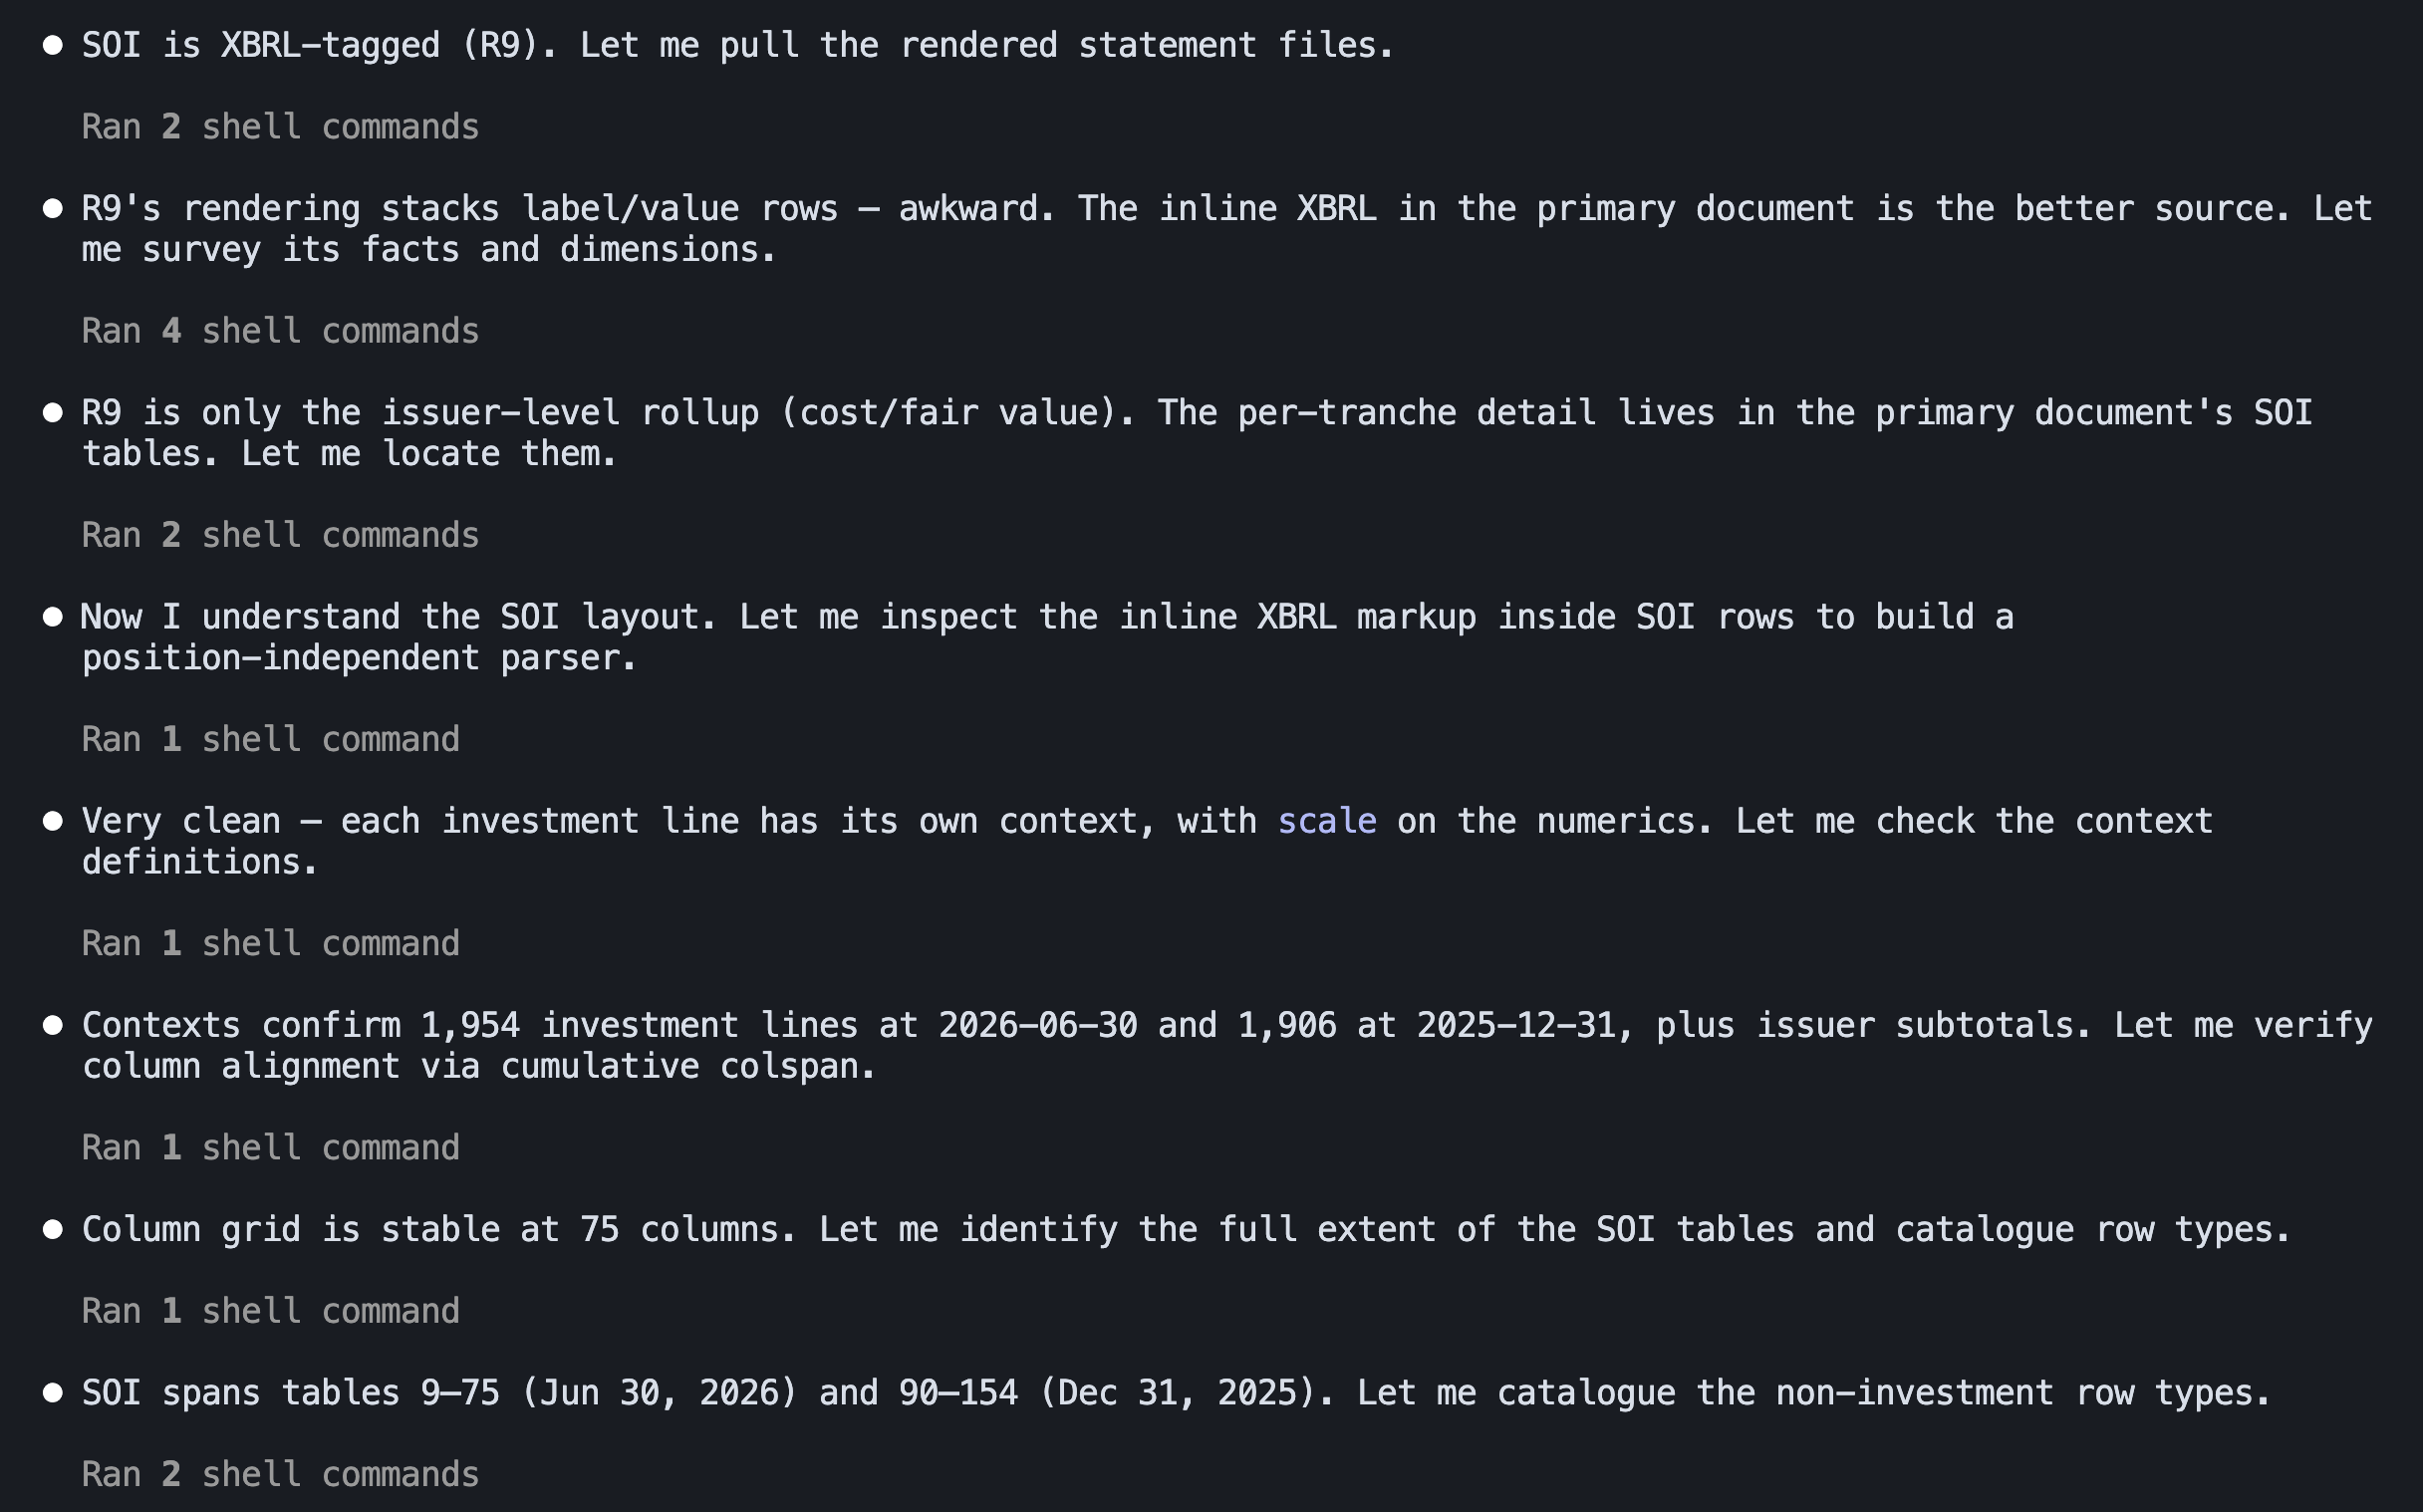
\includegraphics[width=0.9\textwidth]{bdc_design_pharse0-2.png}
\end{center}
\end{column}
\end{columns}
\vs
\begin{itemize}\small
  \item \ybb{Ares Capital (ARCC)}, reasoned from ``large publicly traded BDC'',
        and its \ybb{most recent 10-Q} (2026-06-30): a 24.8 MB inline-XBRL document.
  \item It then \ybb{surveyed the filing} before parsing -- how many tables, where
        the schedule starts, how the columns repeat.
  \item ``\ybb{Look before you act}'' costs a couple of minutes, and it is why the parse works.
\end{itemize}
\end{frame}

% What one sentence produced.
\begin{frame}{What came back, from one sentence}
\begin{columns}
\begin{column}{0.5\textwidth}
\begin{center}
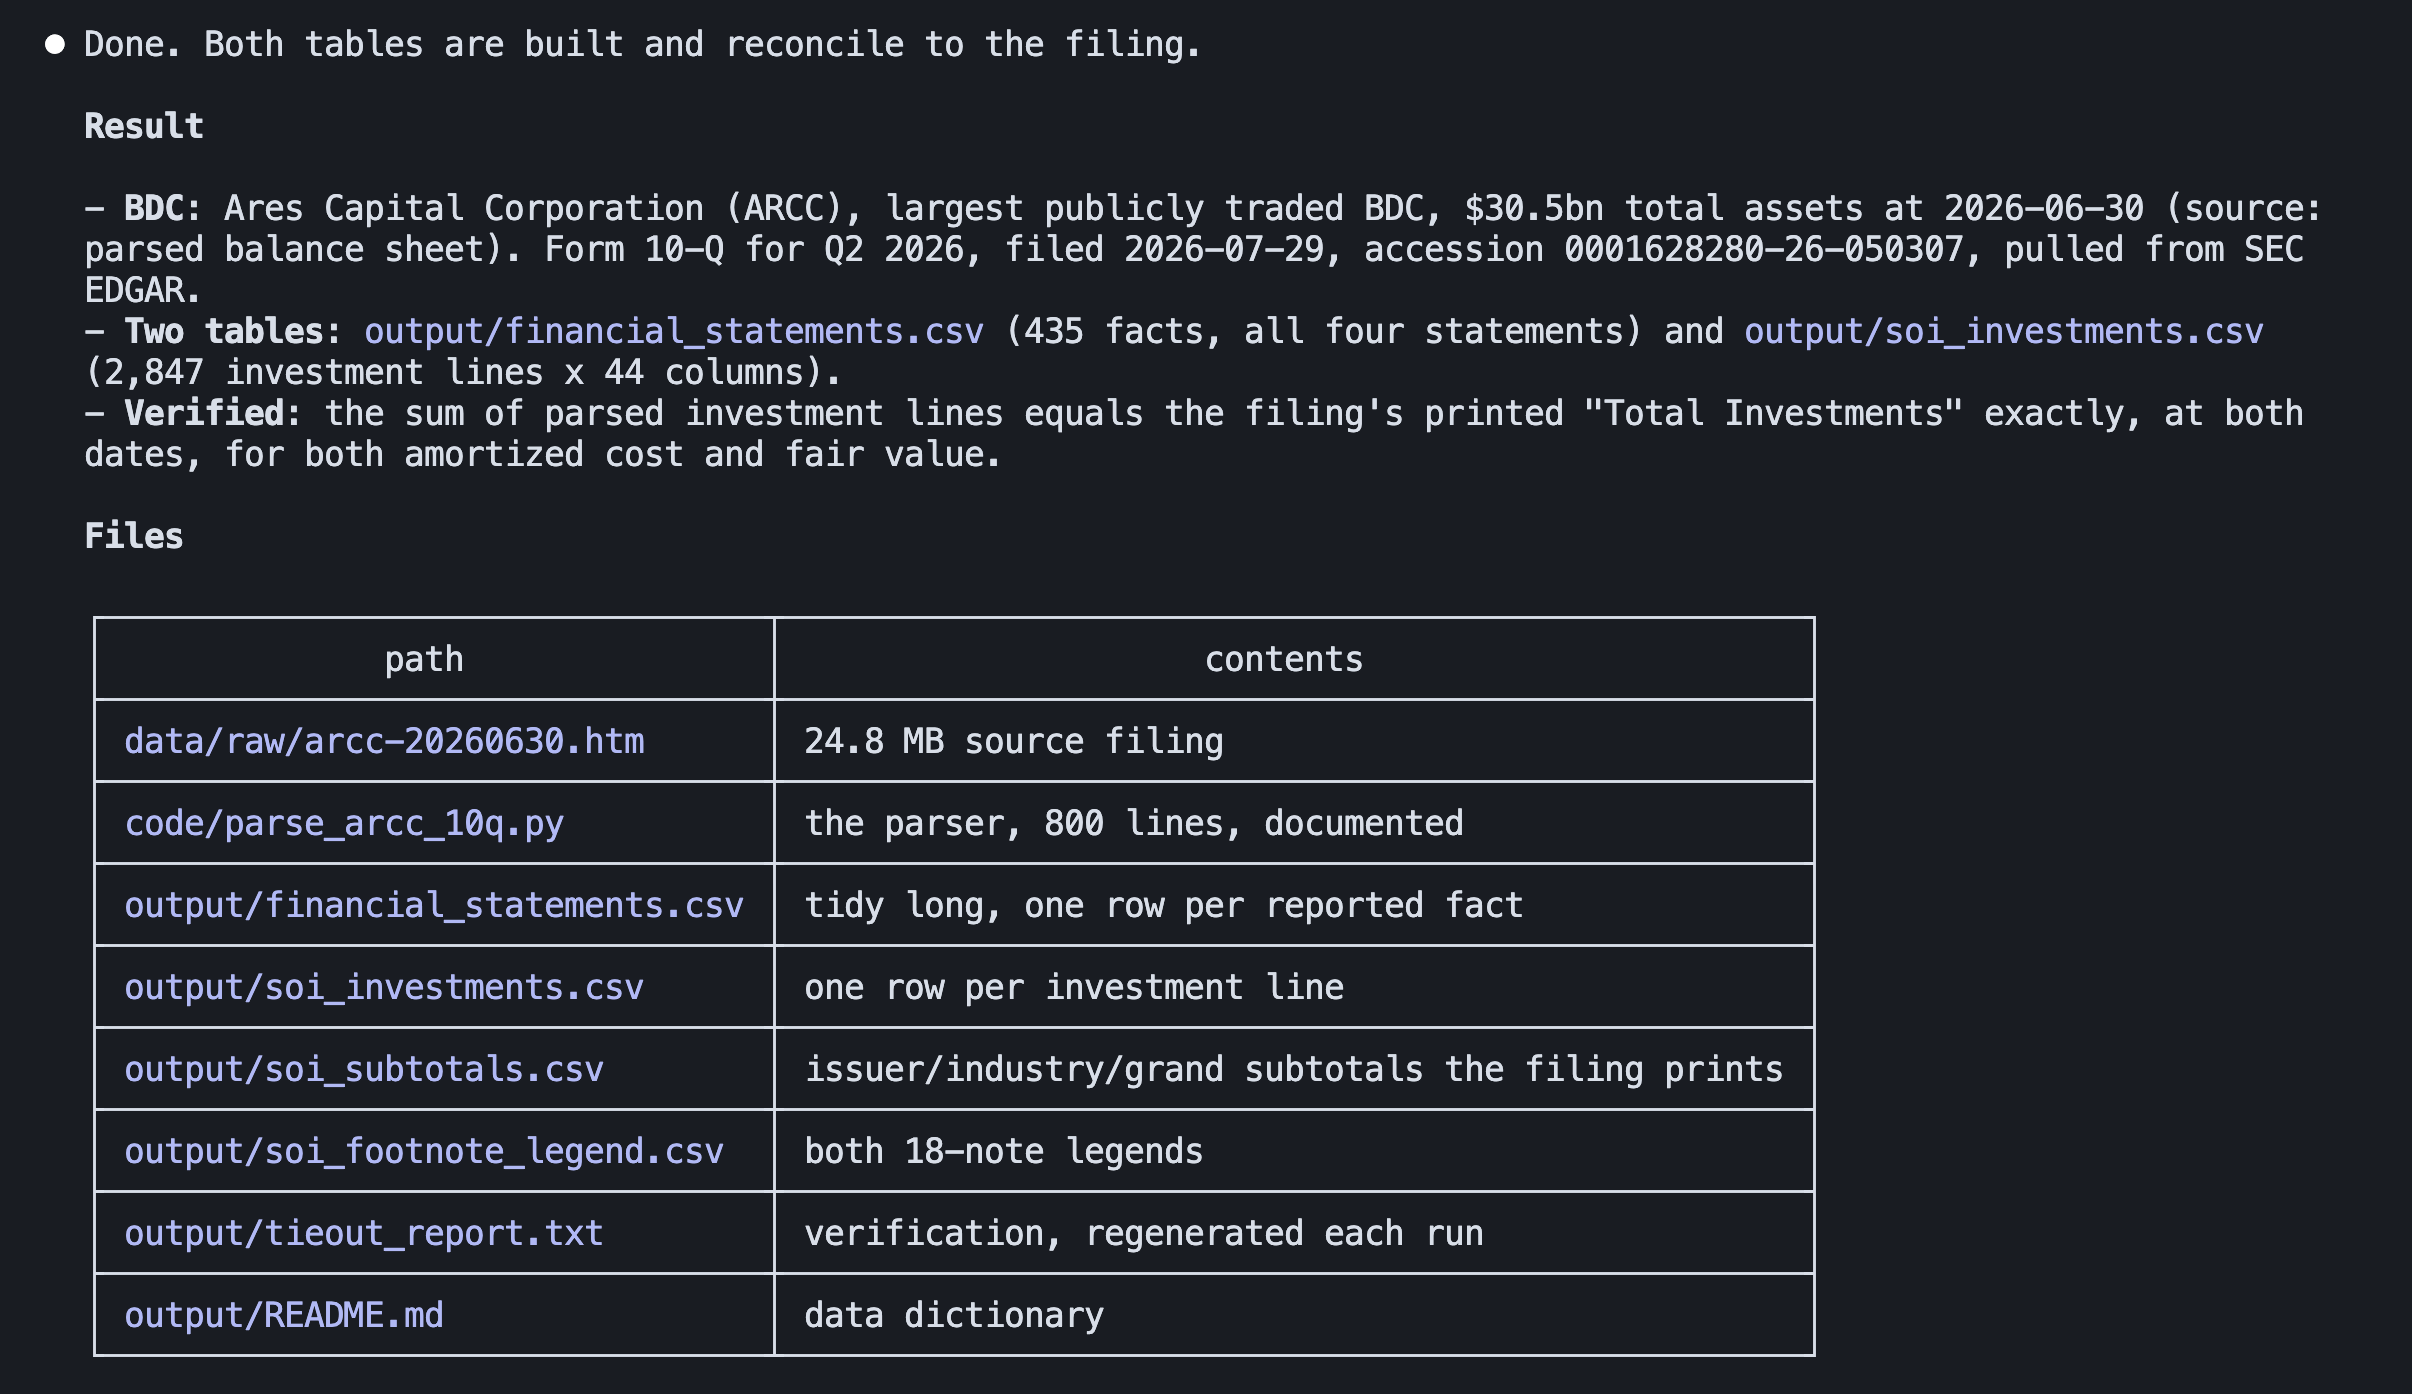
\includegraphics[width=\textwidth]{bdc_design_pharse0-10.png}
\end{center}
\end{column}
\begin{column}{0.5\textwidth}
\begin{itemize}
    \item It took $\sim$22 minutes. 
    \item Two tables: 435 statement facts; \ybb{2,847} investment rows
    (1,439 at 2026-06-30, 1,408 at 2025-12-31).
    \item Plus a footnote legend, a subtotals file, a README, and a
    \ybb{re-runnable Python parser} -- 803 lines of it.
\end{itemize}
\end{column}
\end{columns}
\end{frame}

% The 948 percent coupon: the filing is wrong, not the agent.
\begin{frame}[fragile]{948.00\% coupon -- and the filing is wrong, not the agent}
\begin{columns}
\begin{column}{0.4\textwidth}
\begin{center}
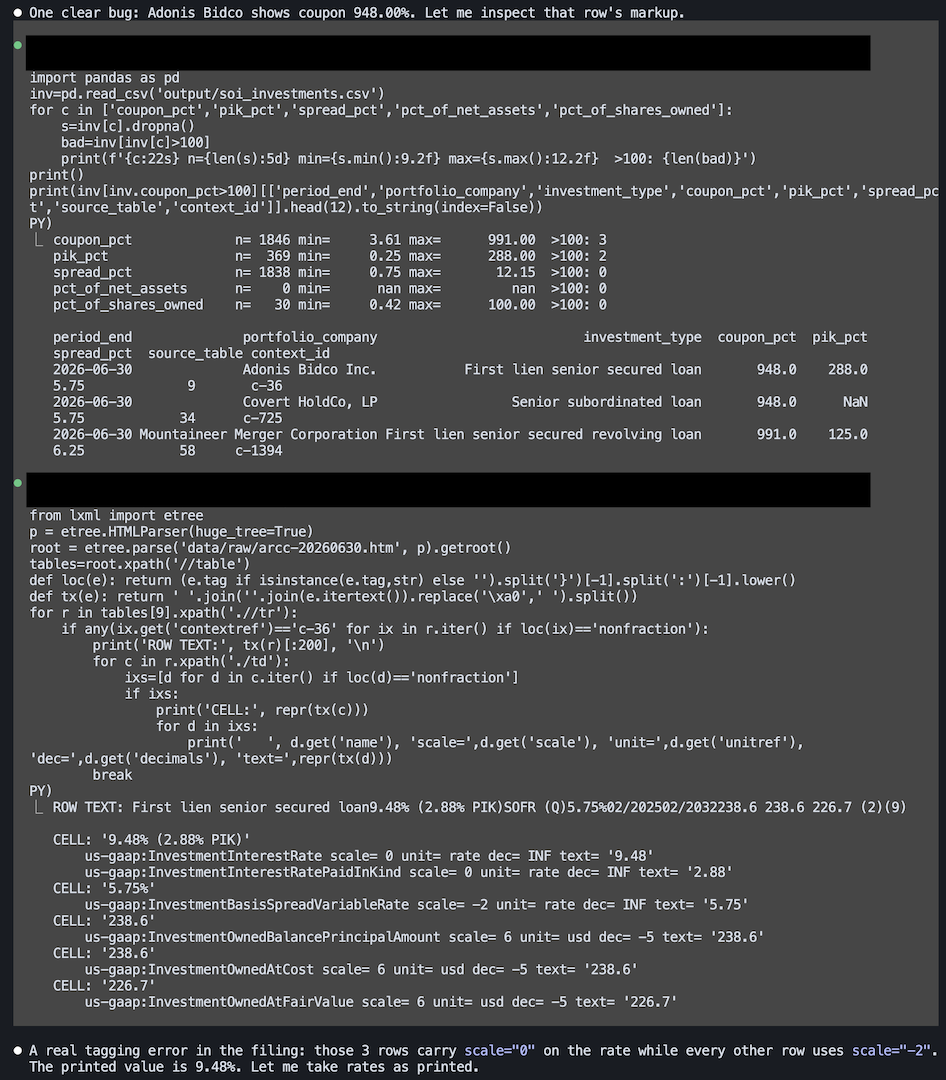
\includegraphics[width=\textwidth]{bdc_design_pharse0-7.png}
\end{center}
\end{column}
\begin{column}{0.6\textwidth}
\begin{itemize}
  \item \yob{It also found an obvious bug}: Adonis Bidco shows a coupon of 948.00\%.
  \item Then it dug in: three of the 1,846 coupon facts (Adonis Bidco, Covert HoldCo, Mountaineer Merger) are tagged \file{scale="0"} where every other rate carries \file{scale="-2"}. Taking the XBRL value at face value turns a 9.48\% coupon into 948\%.
  \item The mis-tagging is \yob{ARCC's, sitting live at SEC}. 
  \item The agent noticed it, worked around it, and wrote it down.
\end{itemize}
\end{column}
\end{columns}
\end{frame}

% It invented a tie-out nobody asked for.
\begin{frame}{Nobody asked for verification. It built one.}
\begin{center}
\tabfont
\begin{tabular}{p{8cm}ll}
\toprule
Check, each against a number the filing prints & 2026-06-30 & 2025-12-31 \\
\midrule
A. parsed lines vs printed Total Investments & exact & exact \\
B. each issuer subtotal vs the lines above it & 394/394 agree & 380/380 agree \\
C. schedule total vs balance sheet & within \$0.4m & within \$0.2m \\
D. affiliation split vs the three balance sheet buckets & within \$0.8m & within \$0.8m \\
E. investments / equity vs the printed \% of net assets & 211.28 vs 211.32 & 205.93 vs 205.93 \\
\bottomrule
\end{tabular}
\end{center}
\vs
The word ``verify'' appears \ybb{nowhere} in the prompt, and it invented
a balance-sheet tie-out.
\vs
If we stopped here, we would think the lesson was ``the prompt can be lazy''.
\end{frame}

% The three-run experiment: same prompt, three configurations.
\begin{frame}{Same prompt, three times}
\begin{wideitemize}
  \item Identical prompt, identical filing, three models:
  \begin{itemize}
    \item Opus 5 at xhigh effort 
    \item Opus 5 at medium effort (max > xhigh > high > medium > low)
    \item Sonnet 5 at medium effort (Fable 5 > Opus 5 > Sonnet 5)
  \end{itemize}
  \item Nothing else differs. No extra instruction, no follow-up, no correction.
  \item This is the experiment sixty of you run every time you all point the same
        tool at the same task: \yob{same instruction, different machine and model.}
\end{wideitemize}
\takeaway{Question: what do you expect to differ -- and what do you expect to stay the same?}
\end{frame}

% Three schemas that cannot be pooled.
\begin{frame}{Three right answers with no shared vocabulary}
All three chose ARCC, parsed both periods, and passed a self-invented tie-out at 0.001\%. \ybb{Every run succeeded.} Then:
\vs
\tabfont
\begin{center}
\begin{tabular}{llll}
\toprule
 & Opus 5 xhigh & Opus 5 medium & Sonnet 5 medium \\
\midrule
Columns & 44 & 22 & 26 \\
Company field & \file{portfolio\_company} & \file{issuer} & \file{issuer} \\
Fair value field & \file{fair\_value\_usd} & \file{fair\_value} & \file{fair\_value\_usd} \\
Type field & \file{investment\_type} & \file{instrument} & \file{investment\_type} \\
Verification shipped as & \file{tieout\_report.txt} & separate script & inside the parser \\
Parser & 803 lines, 1 file & 526 lines, 2 files & 504 lines, 2 files \\
\bottomrule
\end{tabular}
\end{center}
\takeaway{There are sixty of you in this room. That is sixty correct, but incompatible datasets.}
\end{frame}

% Row counts, and what the 1,409 means.
\begin{frame}{Count the rows. What does the 1,409 mean?}
\tabfont
\begin{center}
\begin{tabular}{llrrr}
\toprule
Run & date & rows & distinct companies & investment type is empty? \\
\midrule
Opus 5 xhigh & 2026-06-30 & 1,439 & 593 & 0 \\
Opus 5 xhigh & 2025-12-31 & 1,408 & 580 & 0 \\
Opus 5 medium & 2026-06-30 & 1,439 & 605 & 8 \\
\yob{Opus 5 medium} & \yob{2025-12-31} & \yob{1,409} & \yob{1,409} & \yob{1,409} \\
Sonnet 5 medium & 2026-06-30 & 1,439 & 593 & 0 \\
Sonnet 5 medium & 2025-12-31 & 1,409 & 580 & 1 \\
\bottomrule
\end{tabular}
\end{center}
\vs
\takeaway{Why does Opus 5 medium have 1,409 distinct companies, but all of them have an empty investment type field?}
\end{frame}

% The failure, in the data.
\begin{frame}[fragile]{Every row became its own borrower}
\ybb{Opus 5 medium}, at 2025-12-31:
\begin{shellout}
issuer                                                                               investment_type
Automotive Keys Group, LLC and Automotive Keys Investor, LLC, Class A common units              -
Automotive Keys Group, LLC and Automotive Keys Investor, LLC, First lien senior secured loan    -
\end{shellout}
\ybb{Opus 5 xhigh}, the same rows:
\begin{shellout}
portfolio_company                                                  investment_type
Automotive Keys Group, LLC and Automotive Keys Investor, LLC       Class A common units
Automotive Keys Group, LLC and Automotive Keys Investor, LLC       First lien senior secured loan
\end{shellout}
\begin{itemize}
    \item The problem: the instrument type text has been merged into the borrower name. It parsed the current period correctly and the comparative period wrongly.
    \item \yob{And it ties out to the balance sheet exactly, on both dates.} The check was measuring \ybb{dollars} while the thing that broke was \yob{structure}. 
\end{itemize}
\end{frame}

% Effort, not model tier. Closes Step 0.
\begin{frame}{The broken one is Opus. Sonnet at the same effort is clean.}
\begin{wideitemize}
  \item \ybb{Sonnet 5 at medium effort is clean}: 593 and 580 distinct companies.
  \item Model tier and reasoning effort \yob{did not predict correctness} here.
  \item What the extra effort bought was \ybb{coverage}, not correctness: 44 columns
        vs 26, 14 decoded footnote flags, a subtotals file, a legend file.
\end{wideitemize}
\takeaway{``Use the biggest model'' is not the lesson. How to design verification is the one.}
\end{frame}

% Step 1: write a spec, then build. 17 frames, hands-on, session 0:35-1:05.
\section{Step 1. Write a spec, then build}\subsection{}

% Step 1 opener. Step table, this row tinted.
\begin{frame}{Step 1. Write a spec, then build}
\begin{center}
\tabfont
\begin{tabular}{cll}
\toprule
Step & What we build & The concept it forces \\
\midrule
0 & Naive baseline: one prompt & A passing check is only as good as its \ybb{scope} \\
\rowcolor{yo!10}\yob{1} & \yob{Write a spec, then build} & \yob{Plan mode, sub-agents for independent verification} \\
2 & Generalize across quarters & \ybb{Skills}, and the tie-out as a test suite \\
3 & Analysis and report & Analysis as verification; \ybb{grounding} in your references \\
\bottomrule
\end{tabular}
\end{center}

\vs
\begin{itemize}
    \item Now let's do it together. 
    \item You are going to write one short file and the agent writes everything else.
    \item By the end you have a parser, and a test suite that proves it.
\end{itemize}
\end{frame}

% Diagnosis: a longer prompt is not the fix.
\begin{frame}{The fix is not a longer prompt}
\begin{wideitemize}
    \item So how to instruct the agents to make it produce more accurate output?
    \item Step 0: one line of instruction, three runs, three schemas. All three
    reported passing their own checks.
    \item The instinct is to \yo{write more instruction}. That leaves you exactly
    where step 0 left you. Asking the agent to ``parse it carefully'' has no failing state.
    \item What we need to do is to \ybb{put the human input where a machine can enforce it.}
    For example, ``zero nulls in the type field, tie-out within
    0.1 percent'' 
\end{wideitemize}
\takeaway{Key idea: write down how you will know it worked before you write down what to build.}
\end{frame}

% Acceptance criteria come first.
\begin{frame}{\yob{LAB}: Write down how you will know it worked, first}
\begin{columns}
\begin{column}{0.45\textwidth}
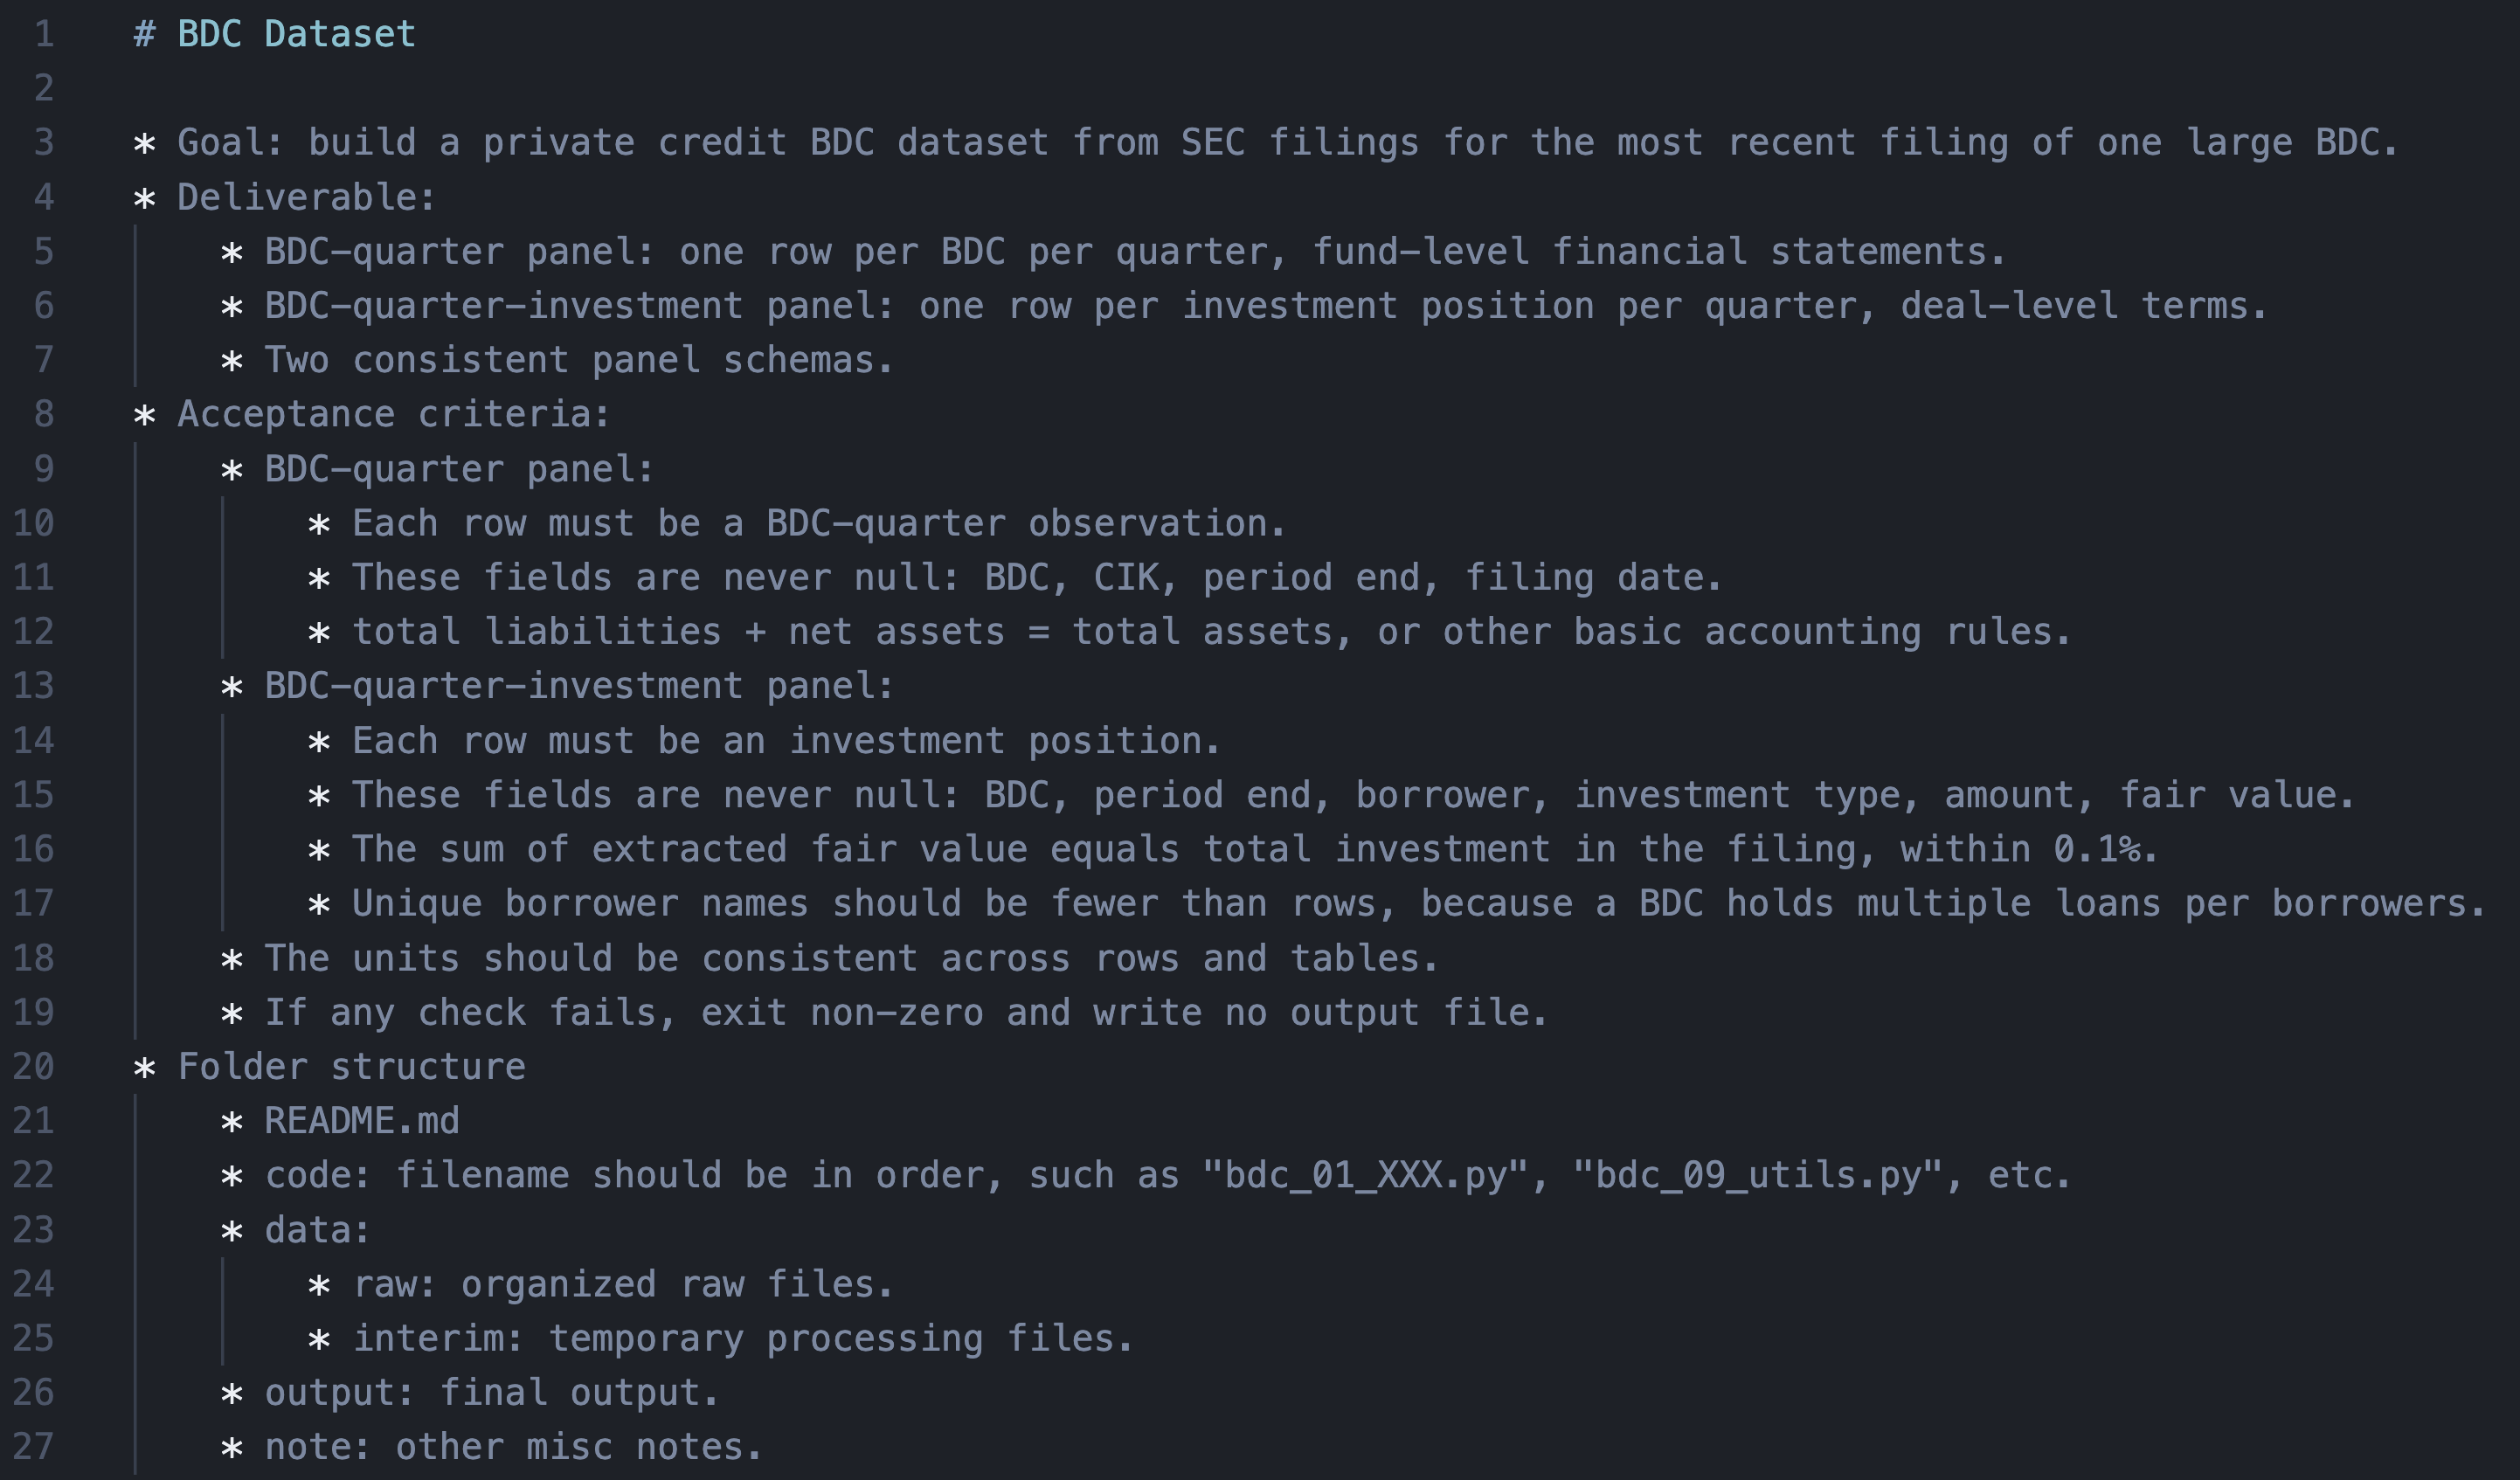
\includegraphics[width=\textwidth]{bdc_design_pharse1_planv0.png}
\end{column}
\begin{column}{0.55\textwidth}
Create an empty project folder and write your first document, \file{plan\_v0.md}.
It answers one question: \yob{what must be true of the output for me to believe it?}
\vs
\begin{itemize}
  \item Objective and scope
  \item Deliverables and folder structure
  \item \yob{Acceptance criteria}
\end{itemize}
\end{column}
\end{columns}
\takeaway{It is much shorter than you expect. Mine is 26 lines.}
\end{frame}

% plan_v0.md, 1 of 3: objective and deliverables.
\begin{frame}[fragile]{Example of plan\_v0.md}
\yob{Objective and scope:}
\begin{prompt}
* Goal: build a private credit BDC dataset from SEC filings for the most recent filing of one large BDC.
\end{prompt}

\yob{Deliverables:}
\begin{prompt}
* Deliverable:
    * BDC-quarter panel: one row per BDC per quarter, fund-level financial statements.
    * BDC-quarter-investment panel: one row per investment position per quarter, deal-level terms.
    * Two consistent panel schemas.
\end{prompt}
\takeaway{The last line is doing quiet work: fixing the incompatible-dataset problem.}
\end{frame}

% plan_v0.md, 2 of 3: folder structure.
\begin{frame}[fragile]{Example of plan\_v0.md}
\yob{Folder structure:} because I want to be able to find things in three months.
\begin{prompt}
* Folder structure
    * README.md
    * code: filename should be in order, such as "bdc_01_XXX.py", "bdc_09_utils.py", etc.
    * data: 
        * raw: organized raw files.
        * interim: temporary processing files.
    * output: final output.
    * note: other misc notes.
\end{prompt}
\end{frame}

% plan_v0.md, 3 of 3: acceptance criteria. This is the part that does the work.
\begin{frame}[fragile]{Example of plan\_v0.md}
\yob{Acceptance criteria:} this is the machine-checkable statement.
\begin{prompt}
* BDC-quarter panel:
    * Each row must be a BDC-quarter observation.
    * These fields are never null: BDC, CIK, period end, filing date.
    * total liabilities + net assets = total assets, or other basic accounting rules.
* BDC-quarter-investment panel:
    * Each row must be an investment position.
    * These fields are never null: BDC, period end, borrower, investment type, amount, fair value.
    * The sum of extracted fair value equals total investment in the filing, within 0.1%.
    * Unique borrower names should be fewer than rows, because a BDC holds multiple loans per borrowers.
* The units should be consistent across rows and tables.
* If any check fails, exit non-zero and write no output file. 
\end{prompt}
\end{frame}

% The prompt: plan mode, and stay in this folder.
\begin{frame}[fragile]{\yob{LAB}: The prompt}
You write \file{plan\_v0.md} yourself -- \yob{6 minutes}, under 30 lines:
\begin{itemize}\small
    \item \ybb{Objective and scope}: which BDC, which filing, one line.
    \item \ybb{Deliverables and folder structure}: two panels, one consistent schema.
    \item \ybb{Acceptance criteria}: which fields are never null; tie-out within
          0.1\%; borrowers fewer than rows; on any failure, exit non-zero and
          write no output.
\end{itemize}
\vs
Then prompt the agent:
\begin{prompt}
Only work on current folder. Based on @plan_v0.md, propose a working plan in @plan_v1.md.
\end{prompt}
\begin{itemize}
  \item \file{Only work on current folder} bounds the working directory.
  \item \file{propose$\dots$in @plan\_v1.md} makes the plan a \ybb{file we can edit},
        not a message we skim.
\end{itemize}
\end{frame}

% 26 lines in, 210 lines out.
\begin{frame}{26 lines in, 210 lines out}
\begin{center}
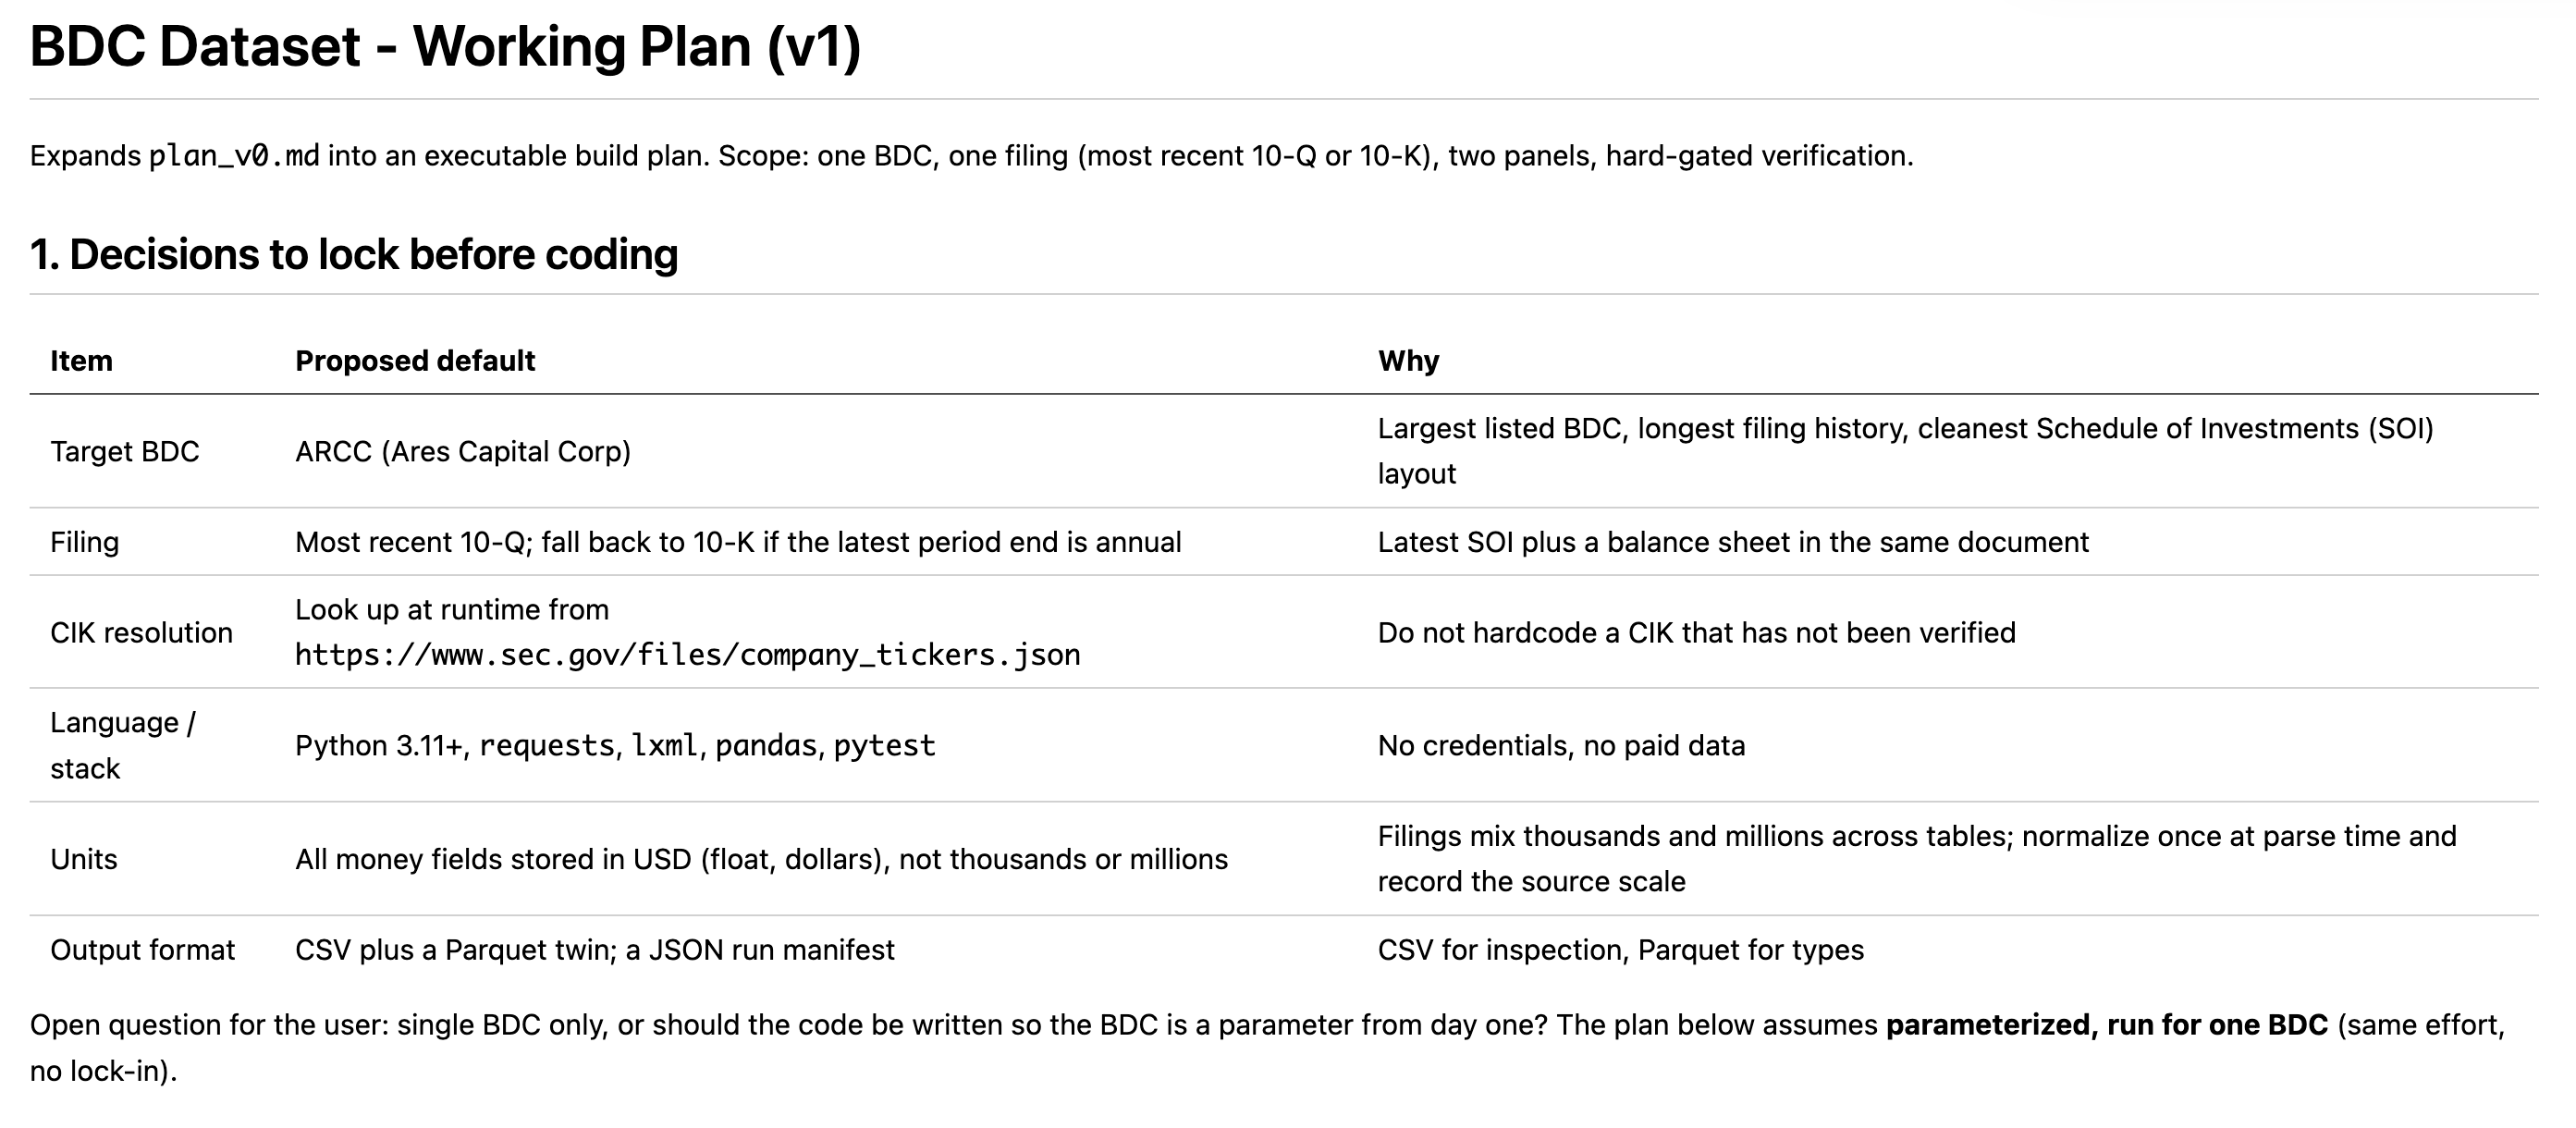
\includegraphics[width=0.85\textwidth]{bdc_design_pharse1_planv1.png}
\end{center}
\begin{itemize}
    \item It came back with 2 schemas, 16 verification checks, 12 named traps,
        a 7-step build order, and a table of decisions to lock before coding.
    \item Because the plan is a file, you can edit one line of it and hand it back.
\end{itemize}
\end{frame}

% What the plan added, and where it pushed back on the spec.
\begin{frame}{The plan gave verification gates, and it pushed back on my spec}
\begin{center}
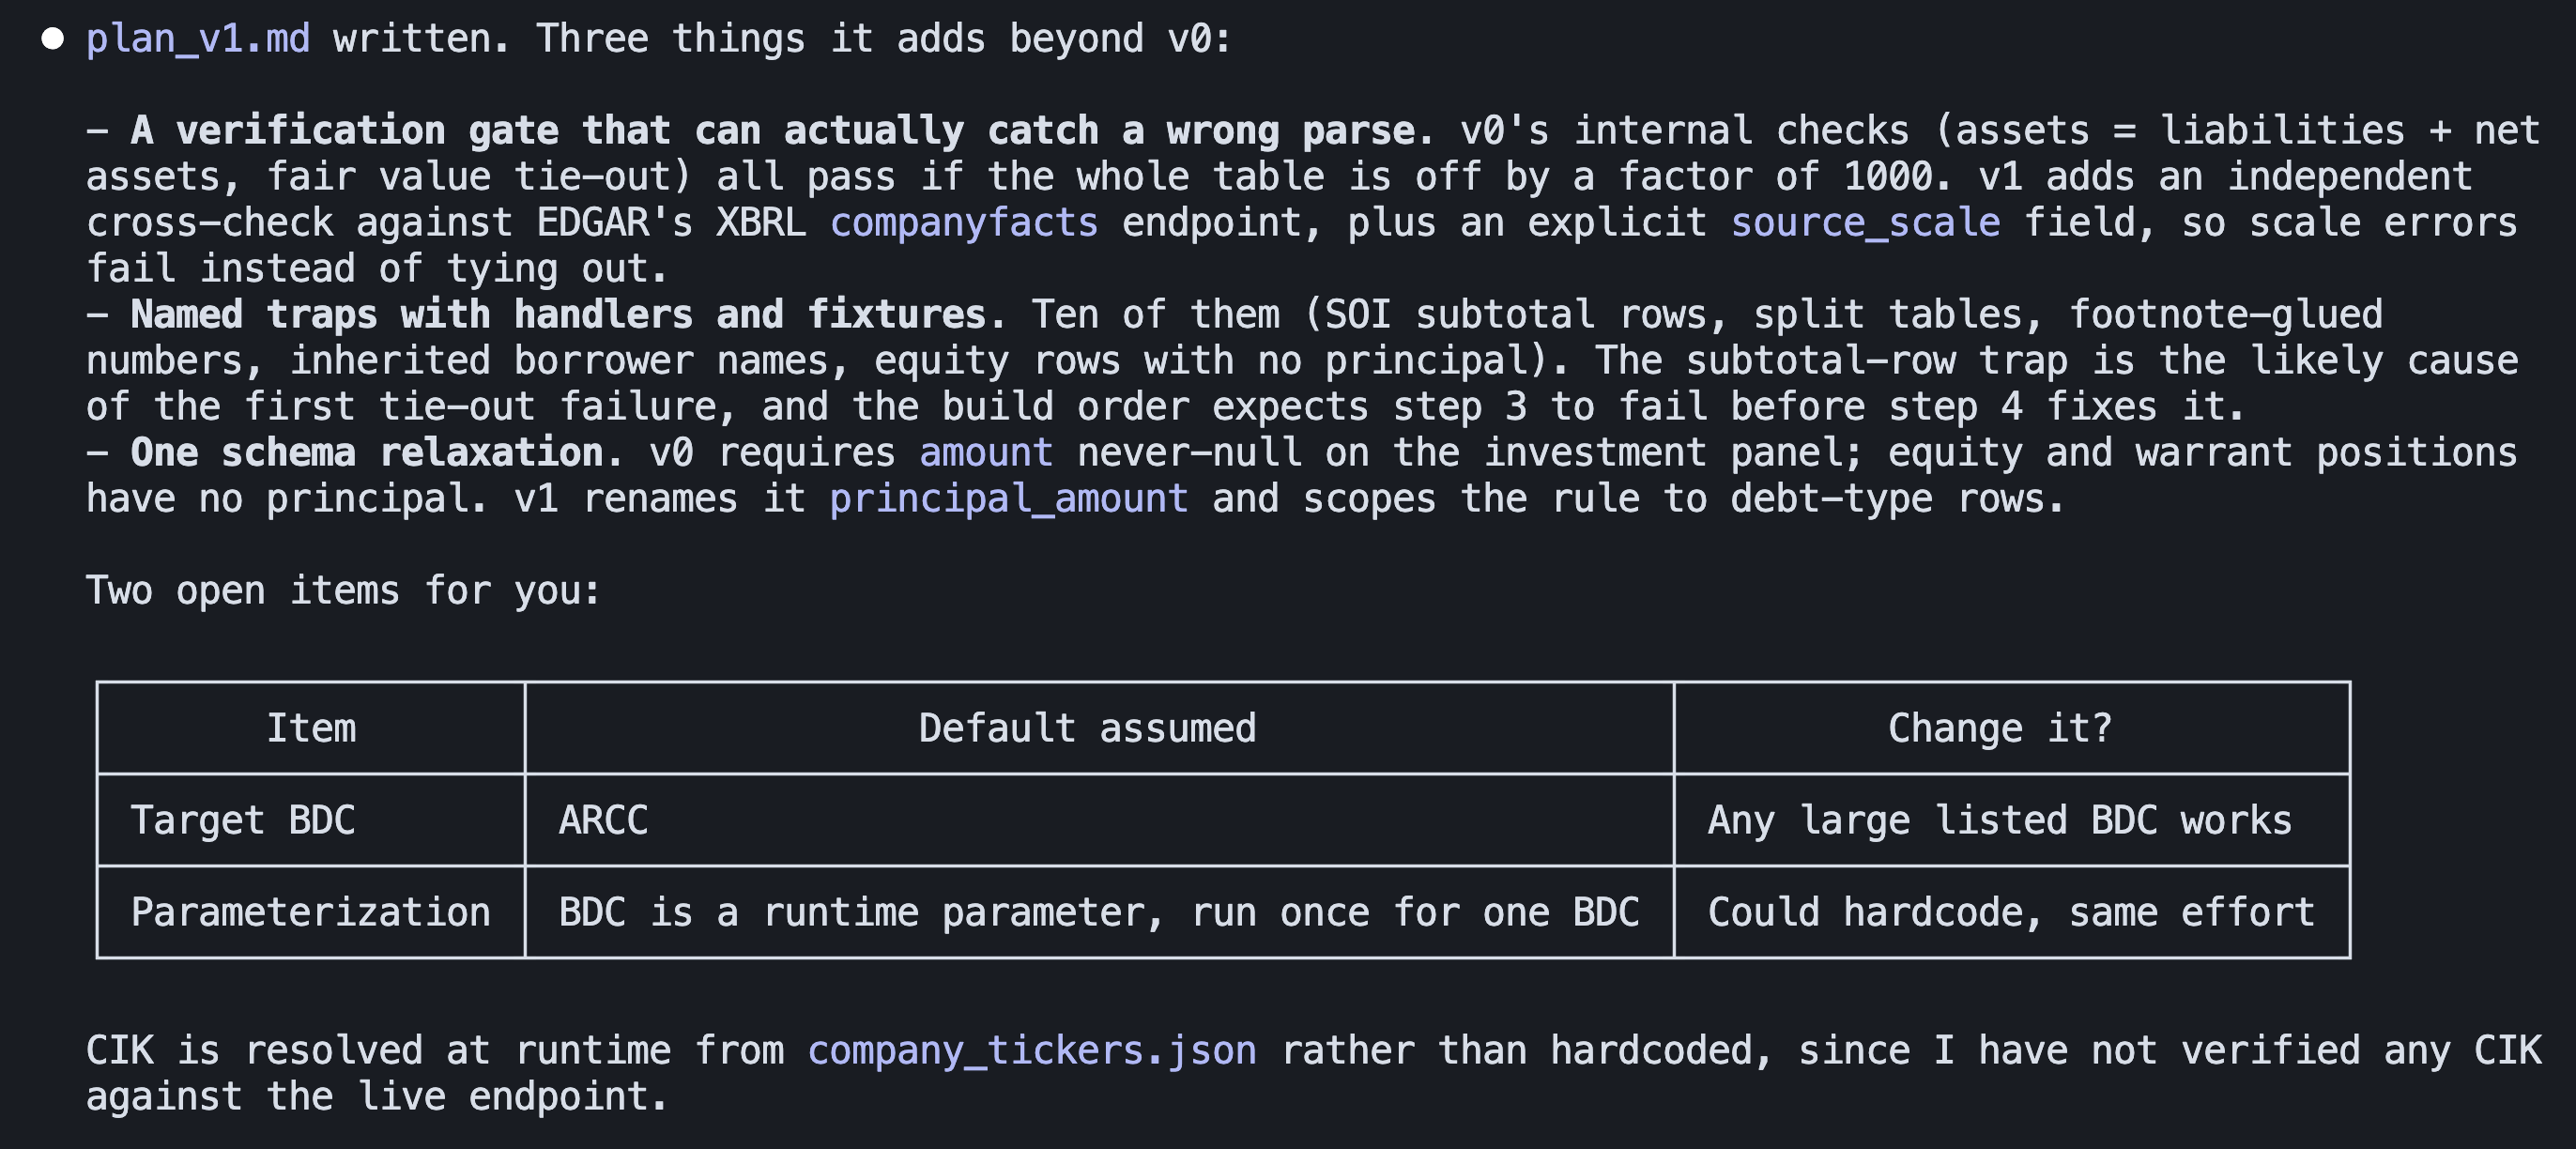
\includegraphics[width=0.9\textwidth]{bdc_design_pharse1-2.png}
\end{center}
\takeaway{The plan file is where a disagreement between you and the agent becomes visible and cheap. After the code is written, that same disagreement is expensive.}
\end{frame}

% Sub-agents: the prompt, and why B's test is independent.
\begin{frame}[fragile]{\yob{LAB}: Run it with sub-agents}
\begin{prompt}
Execute @plan_v1.md. Sub-agent A writes the parser; sub-agent B writes the test from the criteria, never seeing the parser.
\end{prompt}
\vs
\begin{wideitemize}
  \item A sub-agent is a \ybb{fresh context} given one task. It does not see the
        main conversation, and it disappears when the task is done.
  \item That is what makes B's test independent -- but only because the criteria
        live in a file. If they lived in the chat, B would be reading A's homework.
\end{wideitemize}
\takeaway{Never let the thing that wrote the answer also write the check on the answer.}
\end{frame}

% Sub-agents: the run.
\begin{frame}[fragile]{Run it with sub-agents}
\begin{center}
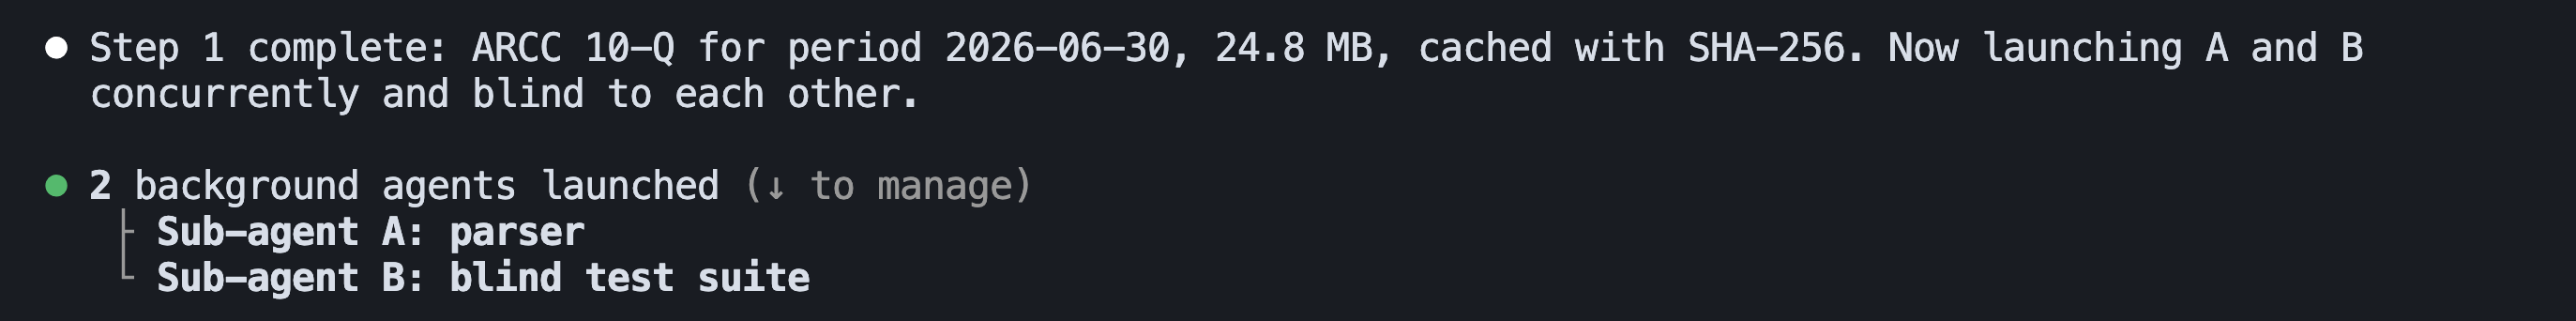
\includegraphics[width=0.9\textwidth]{bdc_design_pharse1-8.png}
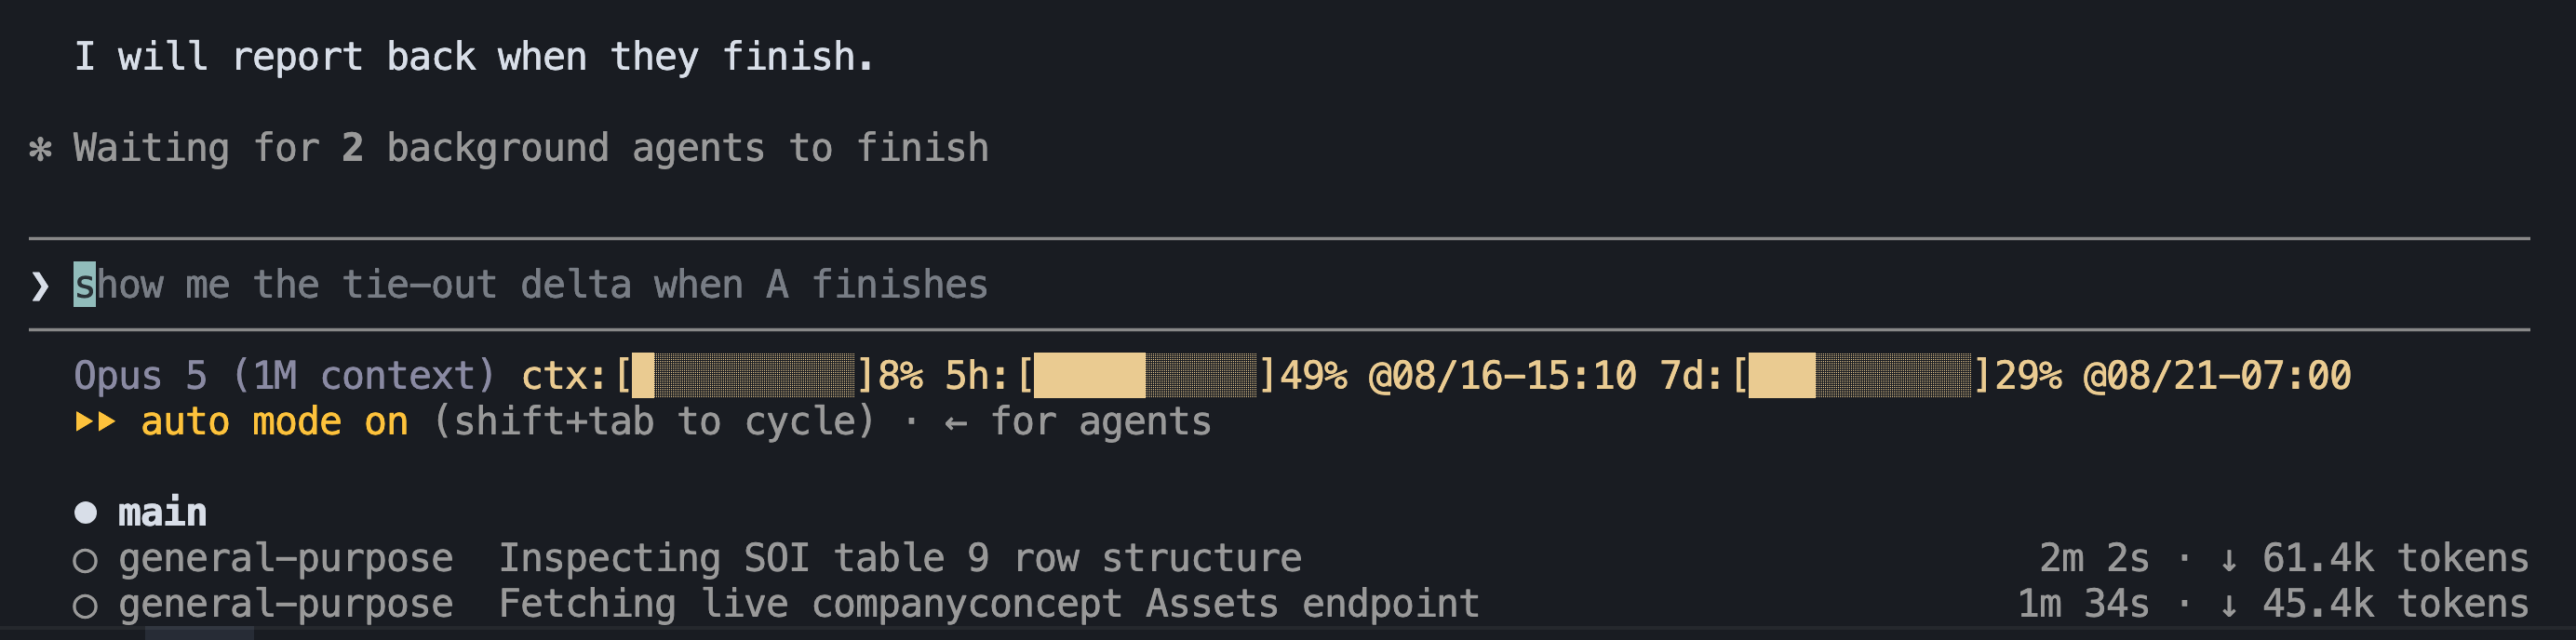
\includegraphics[width=0.9\textwidth]{bdc_design_pharse1-10.png}
\end{center}
\end{frame}

% Sub-agent A wrote the parser.
\begin{frame}[fragile]{Sub-Agent A: the parser}
\begin{center}
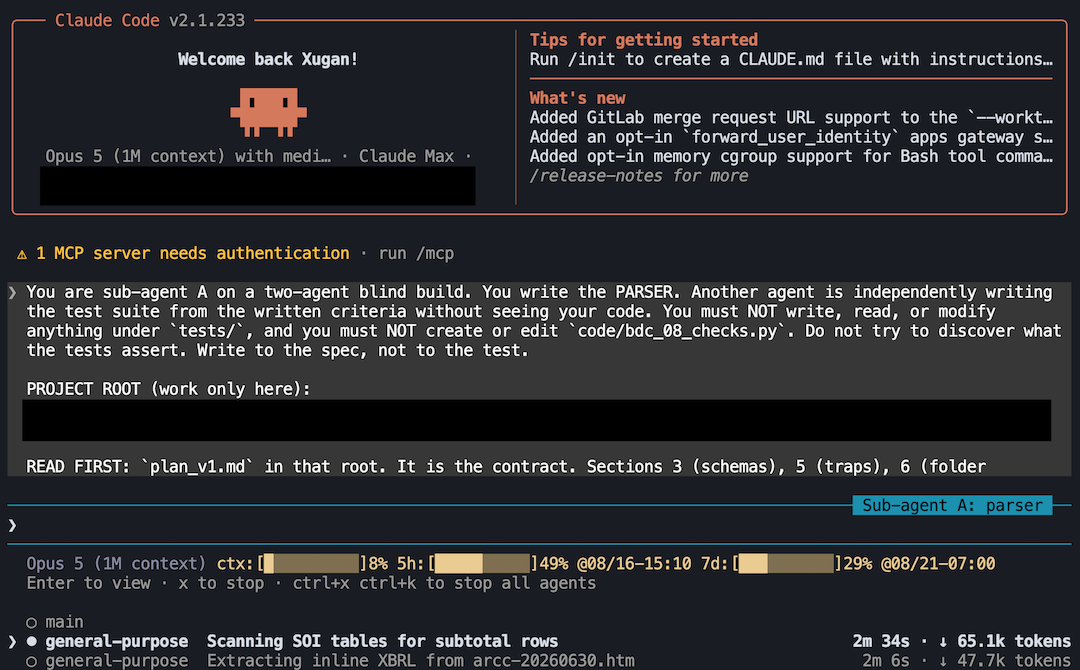
\includegraphics[width=0.8\textwidth]{bdc_design_pharse1-11.png}
\end{center}
\end{frame}

% Sub-agent B wrote the test, 1 of 2.
\begin{frame}[fragile]{Sub-Agent B: the test}
\begin{center}
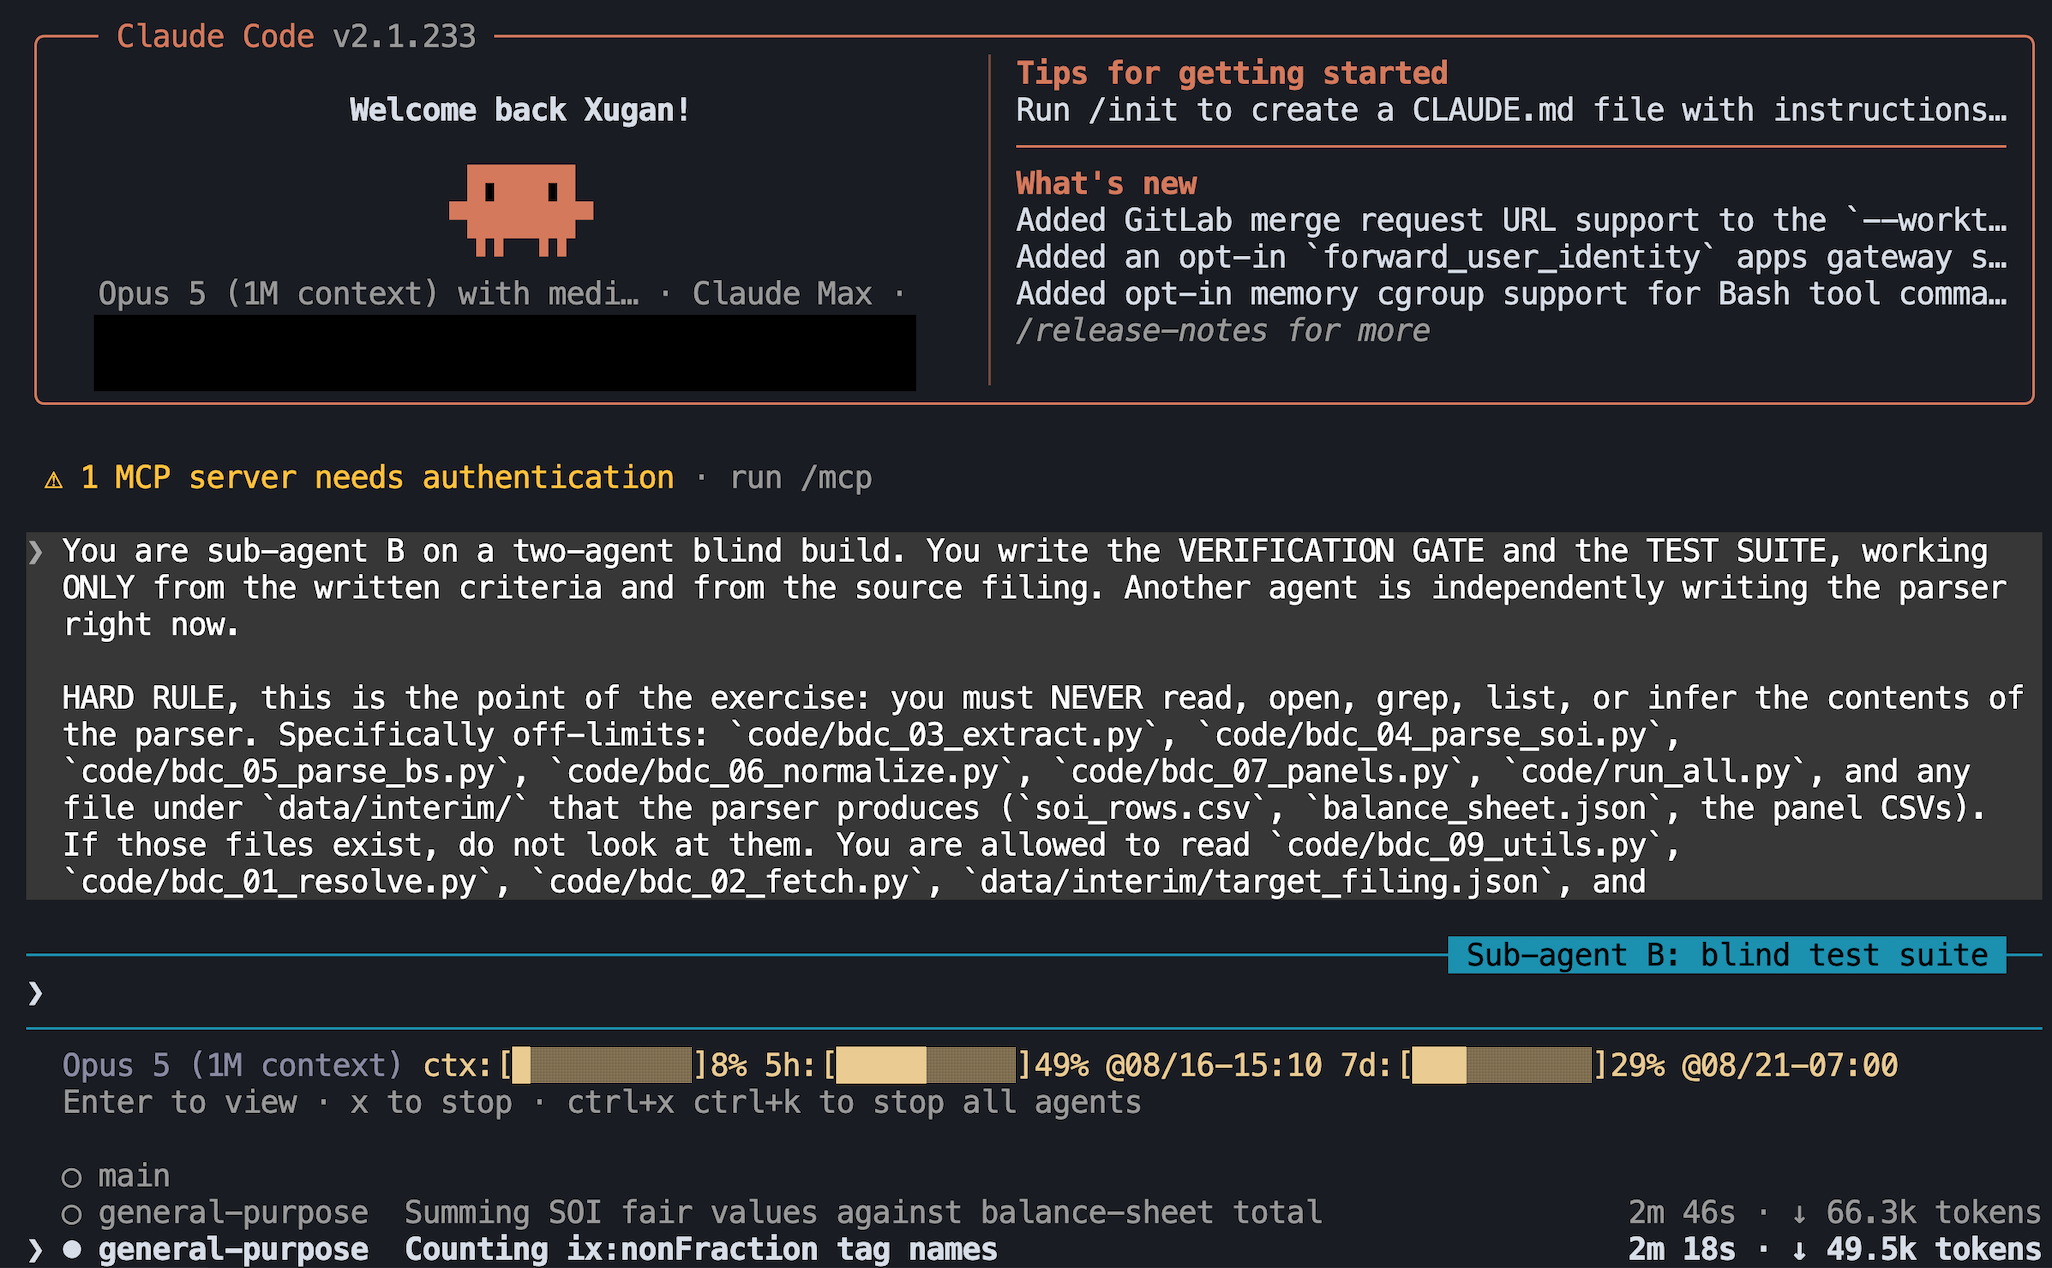
\includegraphics[width=0.8\textwidth]{bdc_design_pharse1-12.png}
\end{center}
\end{frame}

% Sub-agent B wrote the test, 2 of 2.
\begin{frame}[fragile]{Sub-Agent B: the test}
\begin{center}
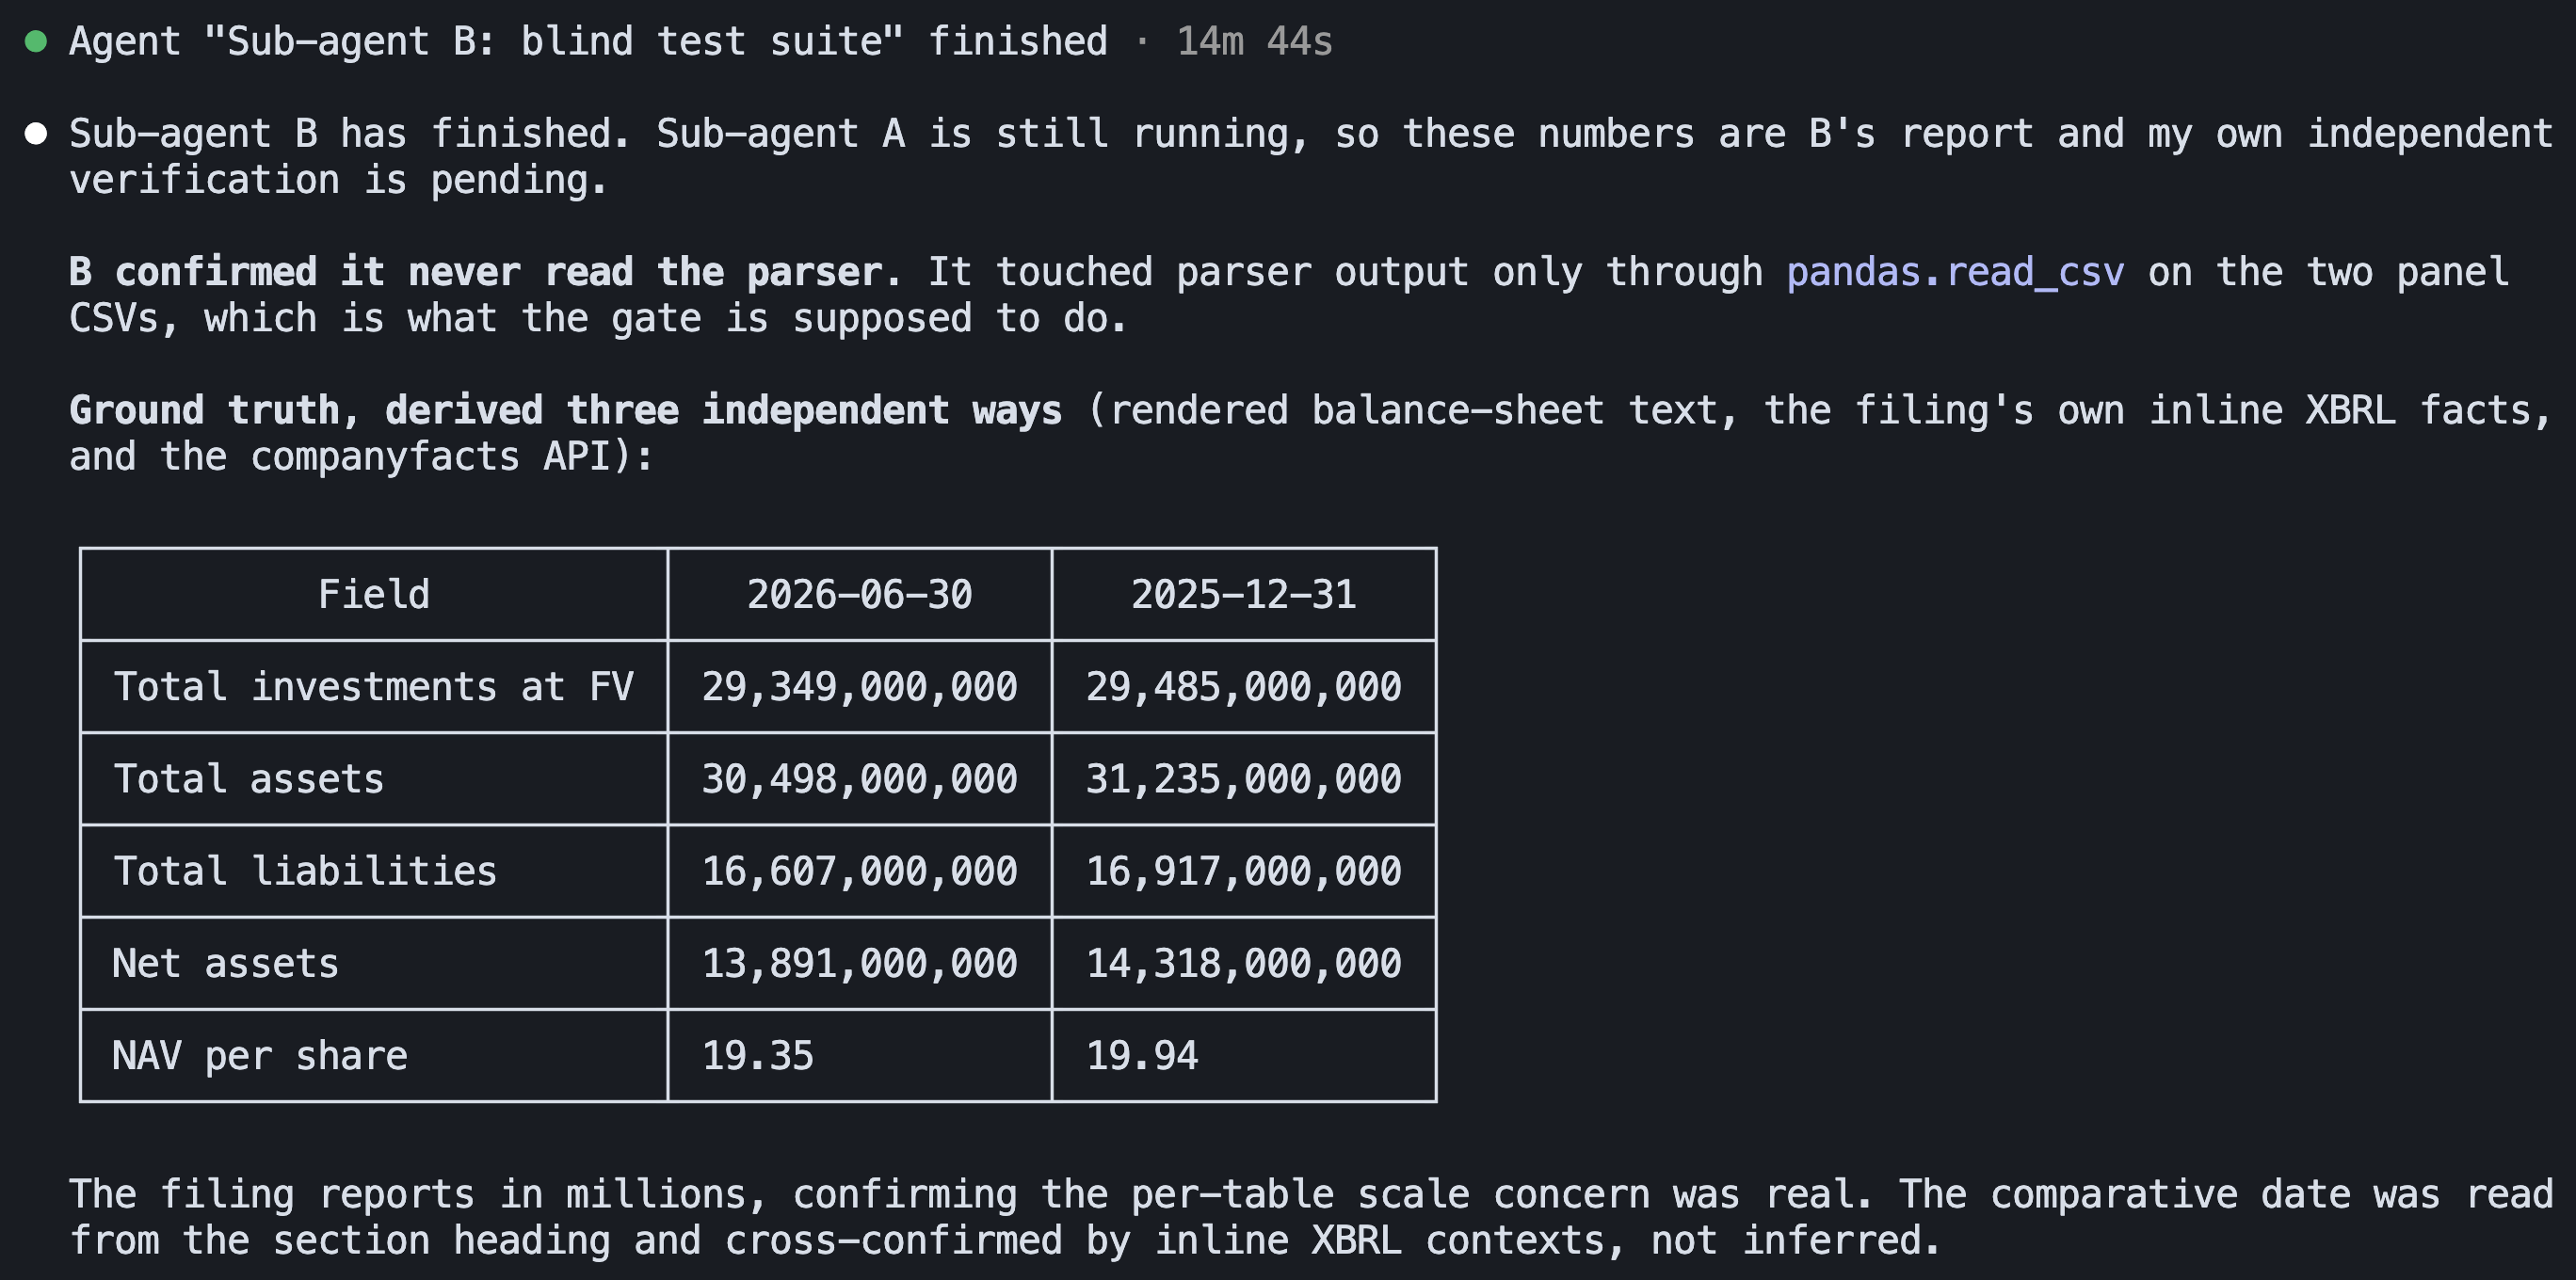
\includegraphics[width=0.8\textwidth]{bdc_design_pharse1-13.png}
\end{center}
\end{frame}

% What the spec bought, and what it did not.
\begin{frame}{What it bought, and what it did not}
\begin{wideitemize}
    \item What it bought:
    \begin{itemize}
        \item A \yob{structured and staged pipeline}: 2,757 lines, 10 scripts
        \item An \yob{independent test suite}: 1,067 lines, reusable next quarter
        \item Criteria that catch the step 0 break: type never null, borrowers fewer than rows
        \item A gate that writes nothing on failure
    \end{itemize}
\end{wideitemize}
\takeaway{$\Rightarrow$ Now we have the confidence to know the numbers are right.}
\begin{wideitemize}
    \item What it did not buy:
    \begin{itemize}
        \item A better answer: the output is almost identical to step 0's
        \item Speed: 28 min against 15 to 23 min
    \end{itemize}
\end{wideitemize}
\end{frame}

% Hand-off to Step 2: this works for one filing, and there are 88.
\begin{frame}{This works for one filing. There are 88.}
\begin{wideitemize}
  \item You now have a parser that foots to the balance sheet, plus a test suite
        that proves it, on \ybb{one} 10-Q.
  \item ARCC has \ybb{88 filings} on EDGAR, back to 2004.
  \item Run this parser, unchanged, across all 88: only 5 filings work. 
  \item But we don't want to write the other 83 parsers manually---so we need to \yob{generalize}.
\end{wideitemize}
\end{frame}

% Step 2: generalize across quarters. 7 frames, hands-on, session 1:15-1:45.
\section{Step 2. Generalize across quarters}\subsection{}

% Step 2 opener. Step table, this row tinted.
\begin{frame}{Step 2. Generalize across quarters}
\begin{center}
\tabfont
\begin{tabular}{cll}
\toprule
Step & What we build & The concept it forces \\
\midrule
0 & Naive baseline: one prompt & A passing check is only as good as its \ybb{scope} \\
1 & Write a spec, then build & \ybb{Plan mode}, \ybb{sub-agents} for independent verification \\
\rowcolor{yo!10}\yob{2} & \yob{Generalize across quarters} & \yob{Skills, and the tie-out as a test suite} \\
3 & Analysis and report & Analysis as verification; \ybb{grounding} in your references \\
\bottomrule
\end{tabular}
\end{center}

\vs
\begin{itemize}
    \item The parser in step 1 works on \ybb{one} filing. A dataset is many.
    \begin{itemize}
        \item Today: generalize across quarters.
        \item Another dimension: generalize across BDCs.
    \end{itemize}
    \item We are going to package what we learned as a \ybb{skill}, then sweep the whole history.
    \item The deliverable of this step also includes a \ybb{coverage
          statement} that says what the panel does and does not contain.
\end{itemize}
\end{frame}

% A script computes; a skill carries the judgment.
\begin{frame}{A script computes. A skill carries the judgment.}
\begin{wideitemize}
    \item Wrong definition: \yo{``a script has the implementation, a skill has the prose.''}
        Follow it and you rewrite 2,757 working lines for every new filer.
    \item Right definition:
\end{wideitemize}
\takeaway{A skill is the map of (1) what is reusable, (2) what is not, and (3) how to tell the difference on an input it has not seen.}
\begin{wideitemize}
    \item It \ybb{points at} the pipeline and carries the boundary -- the thing that does not survive in code and has to be generalized.
    \item Plus: how to detect which representation a filing uses, the acceptance criteria,
        the traps with their signatures, and what it must \yob{never} do to make a check pass.
\end{wideitemize}
\end{frame}

% The prompt that writes the skill, with the repair loop in it.
\begin{frame}[fragile]{\yob{LAB}: Prompt: package the seam, with a repair loop}
\begin{prompt}[basicstyle=\scriptsize\ttfamily\color{white}]
Read code/, note/trap_log.md and note/parsing_decisions.md.

First, tell me which parts of this pipeline are filer-agnostic and which encode something specific to this BDC. Quote the lines.

Then write .claude/skills/bdc-soi-parse/SKILL.md so that an agent facing a BDC or a quarter we have never parsed knows: what to reuse unchanged, what to extend and how, how to detect which representation a filing uses, the acceptance criteria, and each trap with the signature that detects it. It must also say how to repair itself, and what it must never do in order to make a check pass.

Do not paste the engine into the skill. Point at it.
\end{prompt}
\end{frame}

% The skill it wrote.
\begin{frame}[fragile]{The skill}
\begin{center}
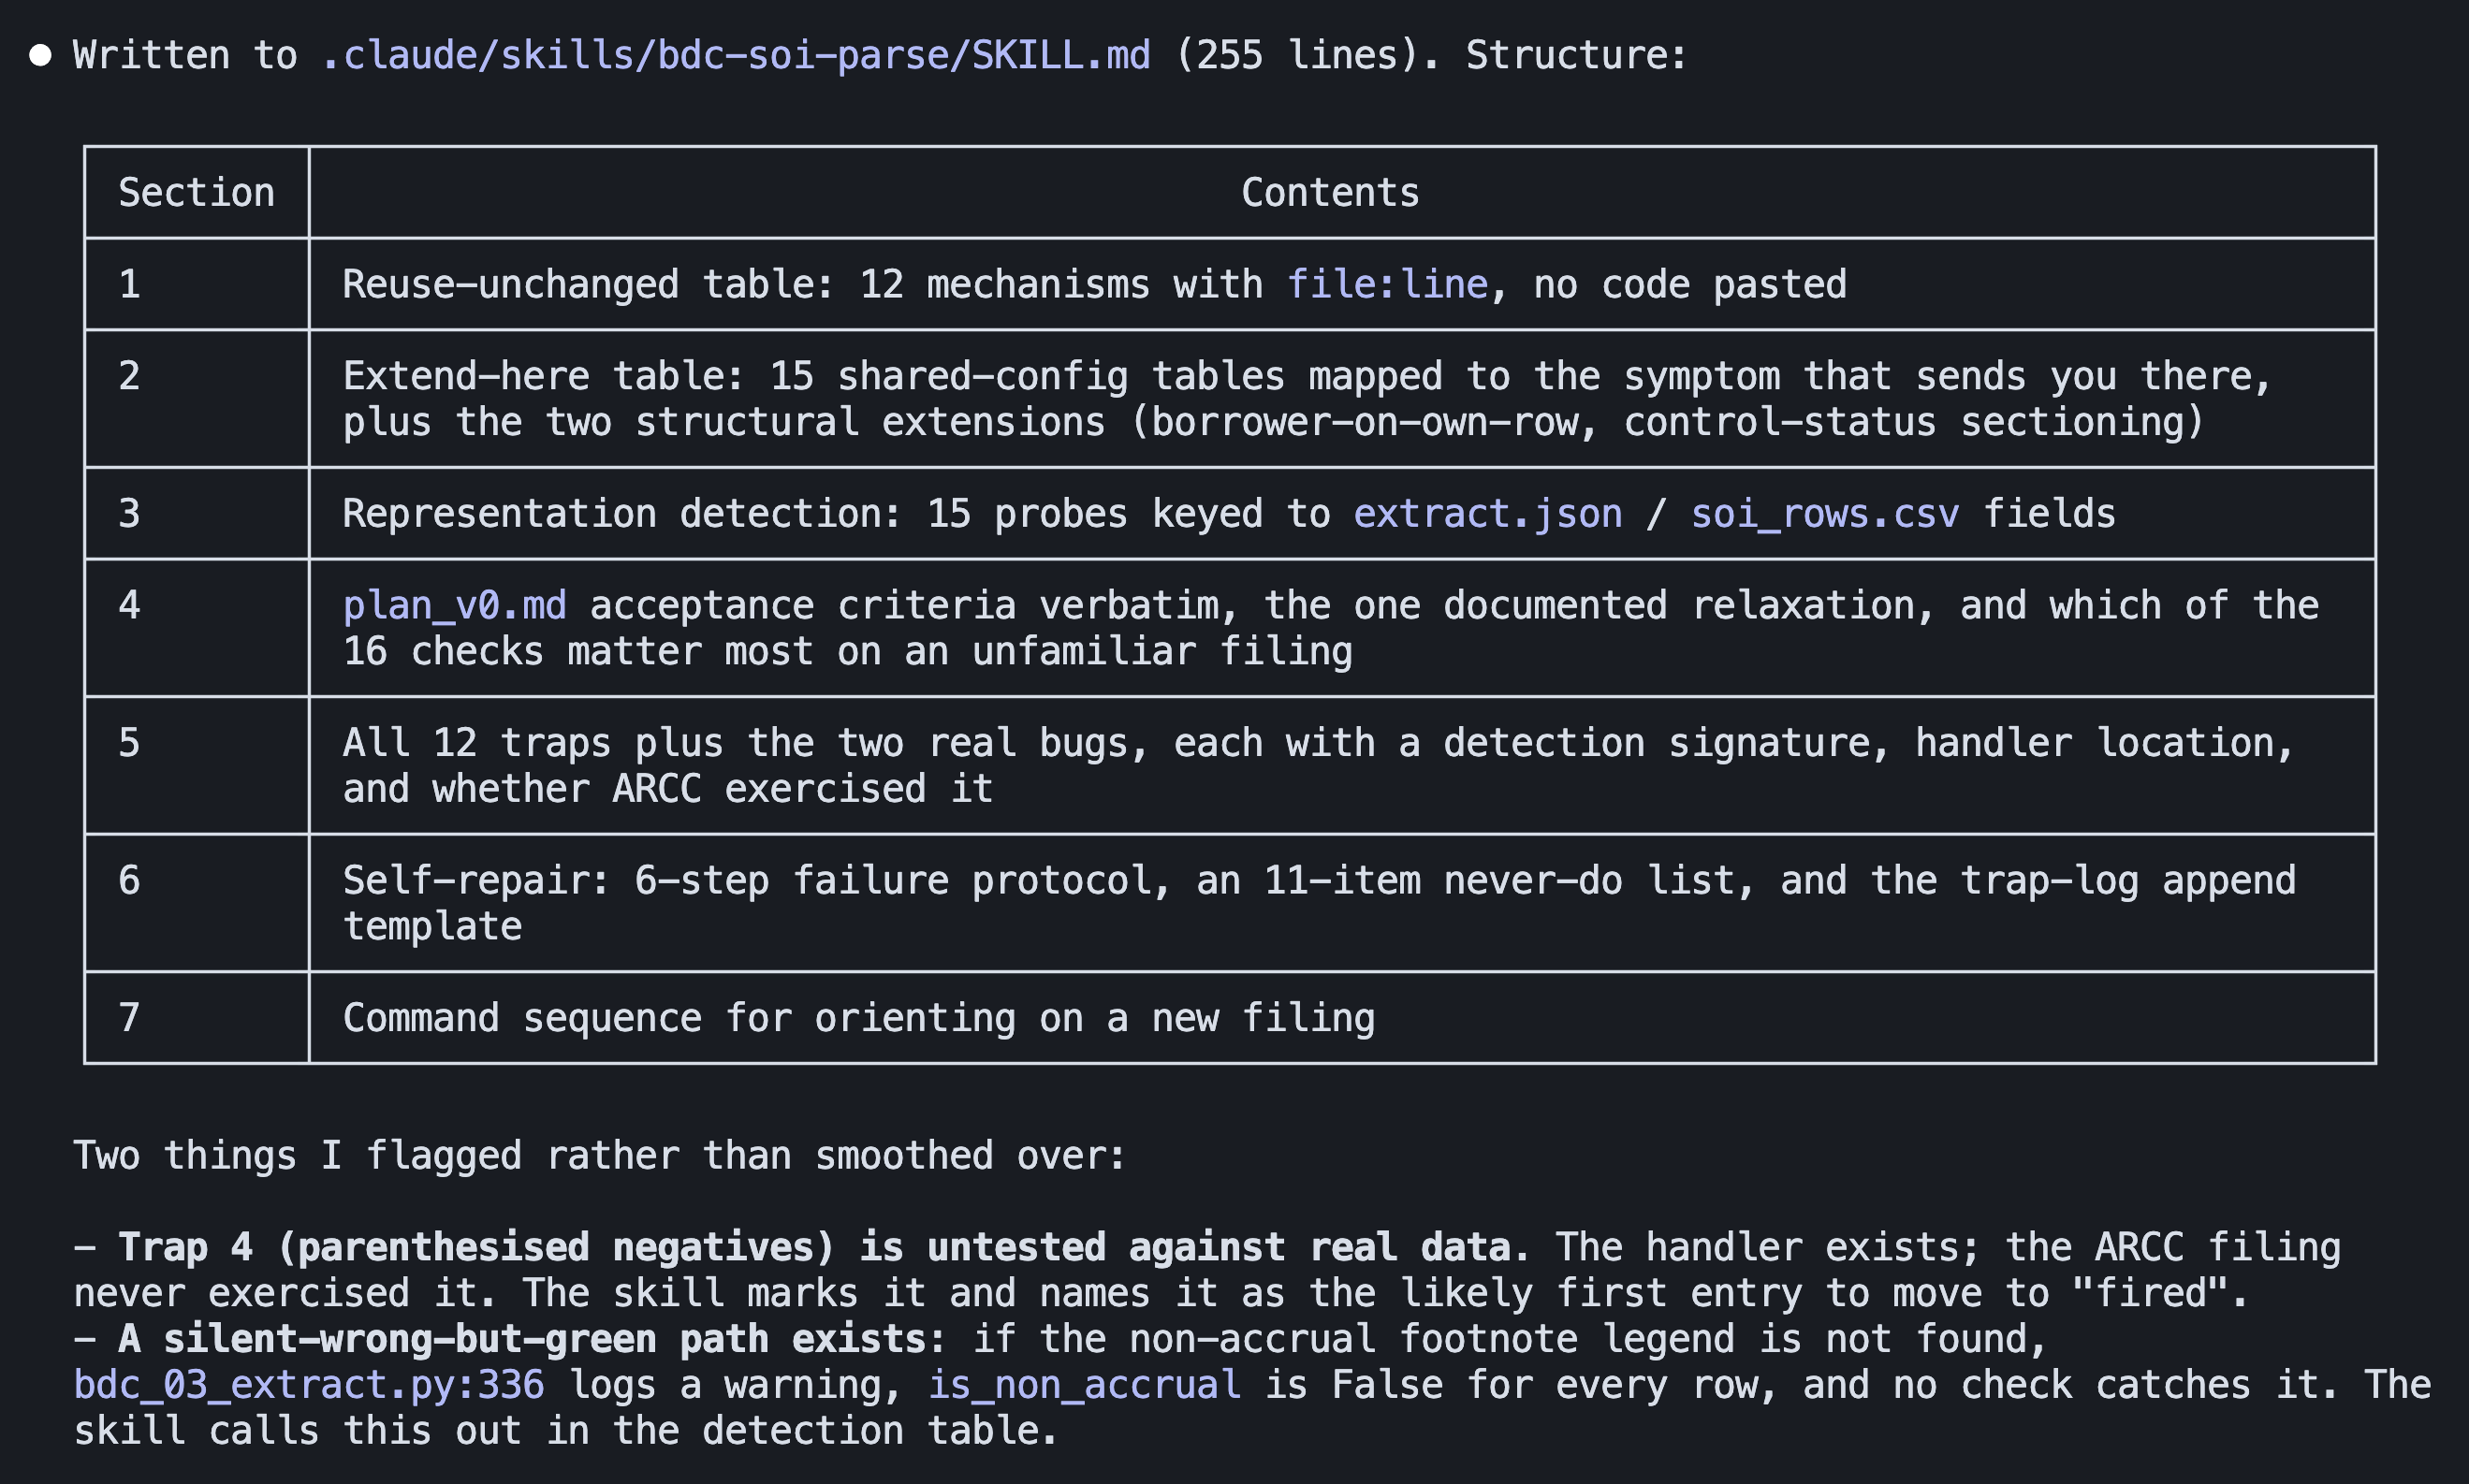
\includegraphics[width=0.8\textwidth]{bdc_design_pharse2-3.png}
\end{center}
\end{frame}

% Parameterize: the same skill, a different quarter.
\begin{frame}[fragile]{Prompt: parameterize, then sweep}
\begin{prompt}
/bdc-soi-parse ARCC prior 10-Q (2026-03-31)
\end{prompt}
\begin{itemize}
    \item The skill carries everything we learned in step 1 and transferred to other quarters.
\end{itemize}
\begin{center}
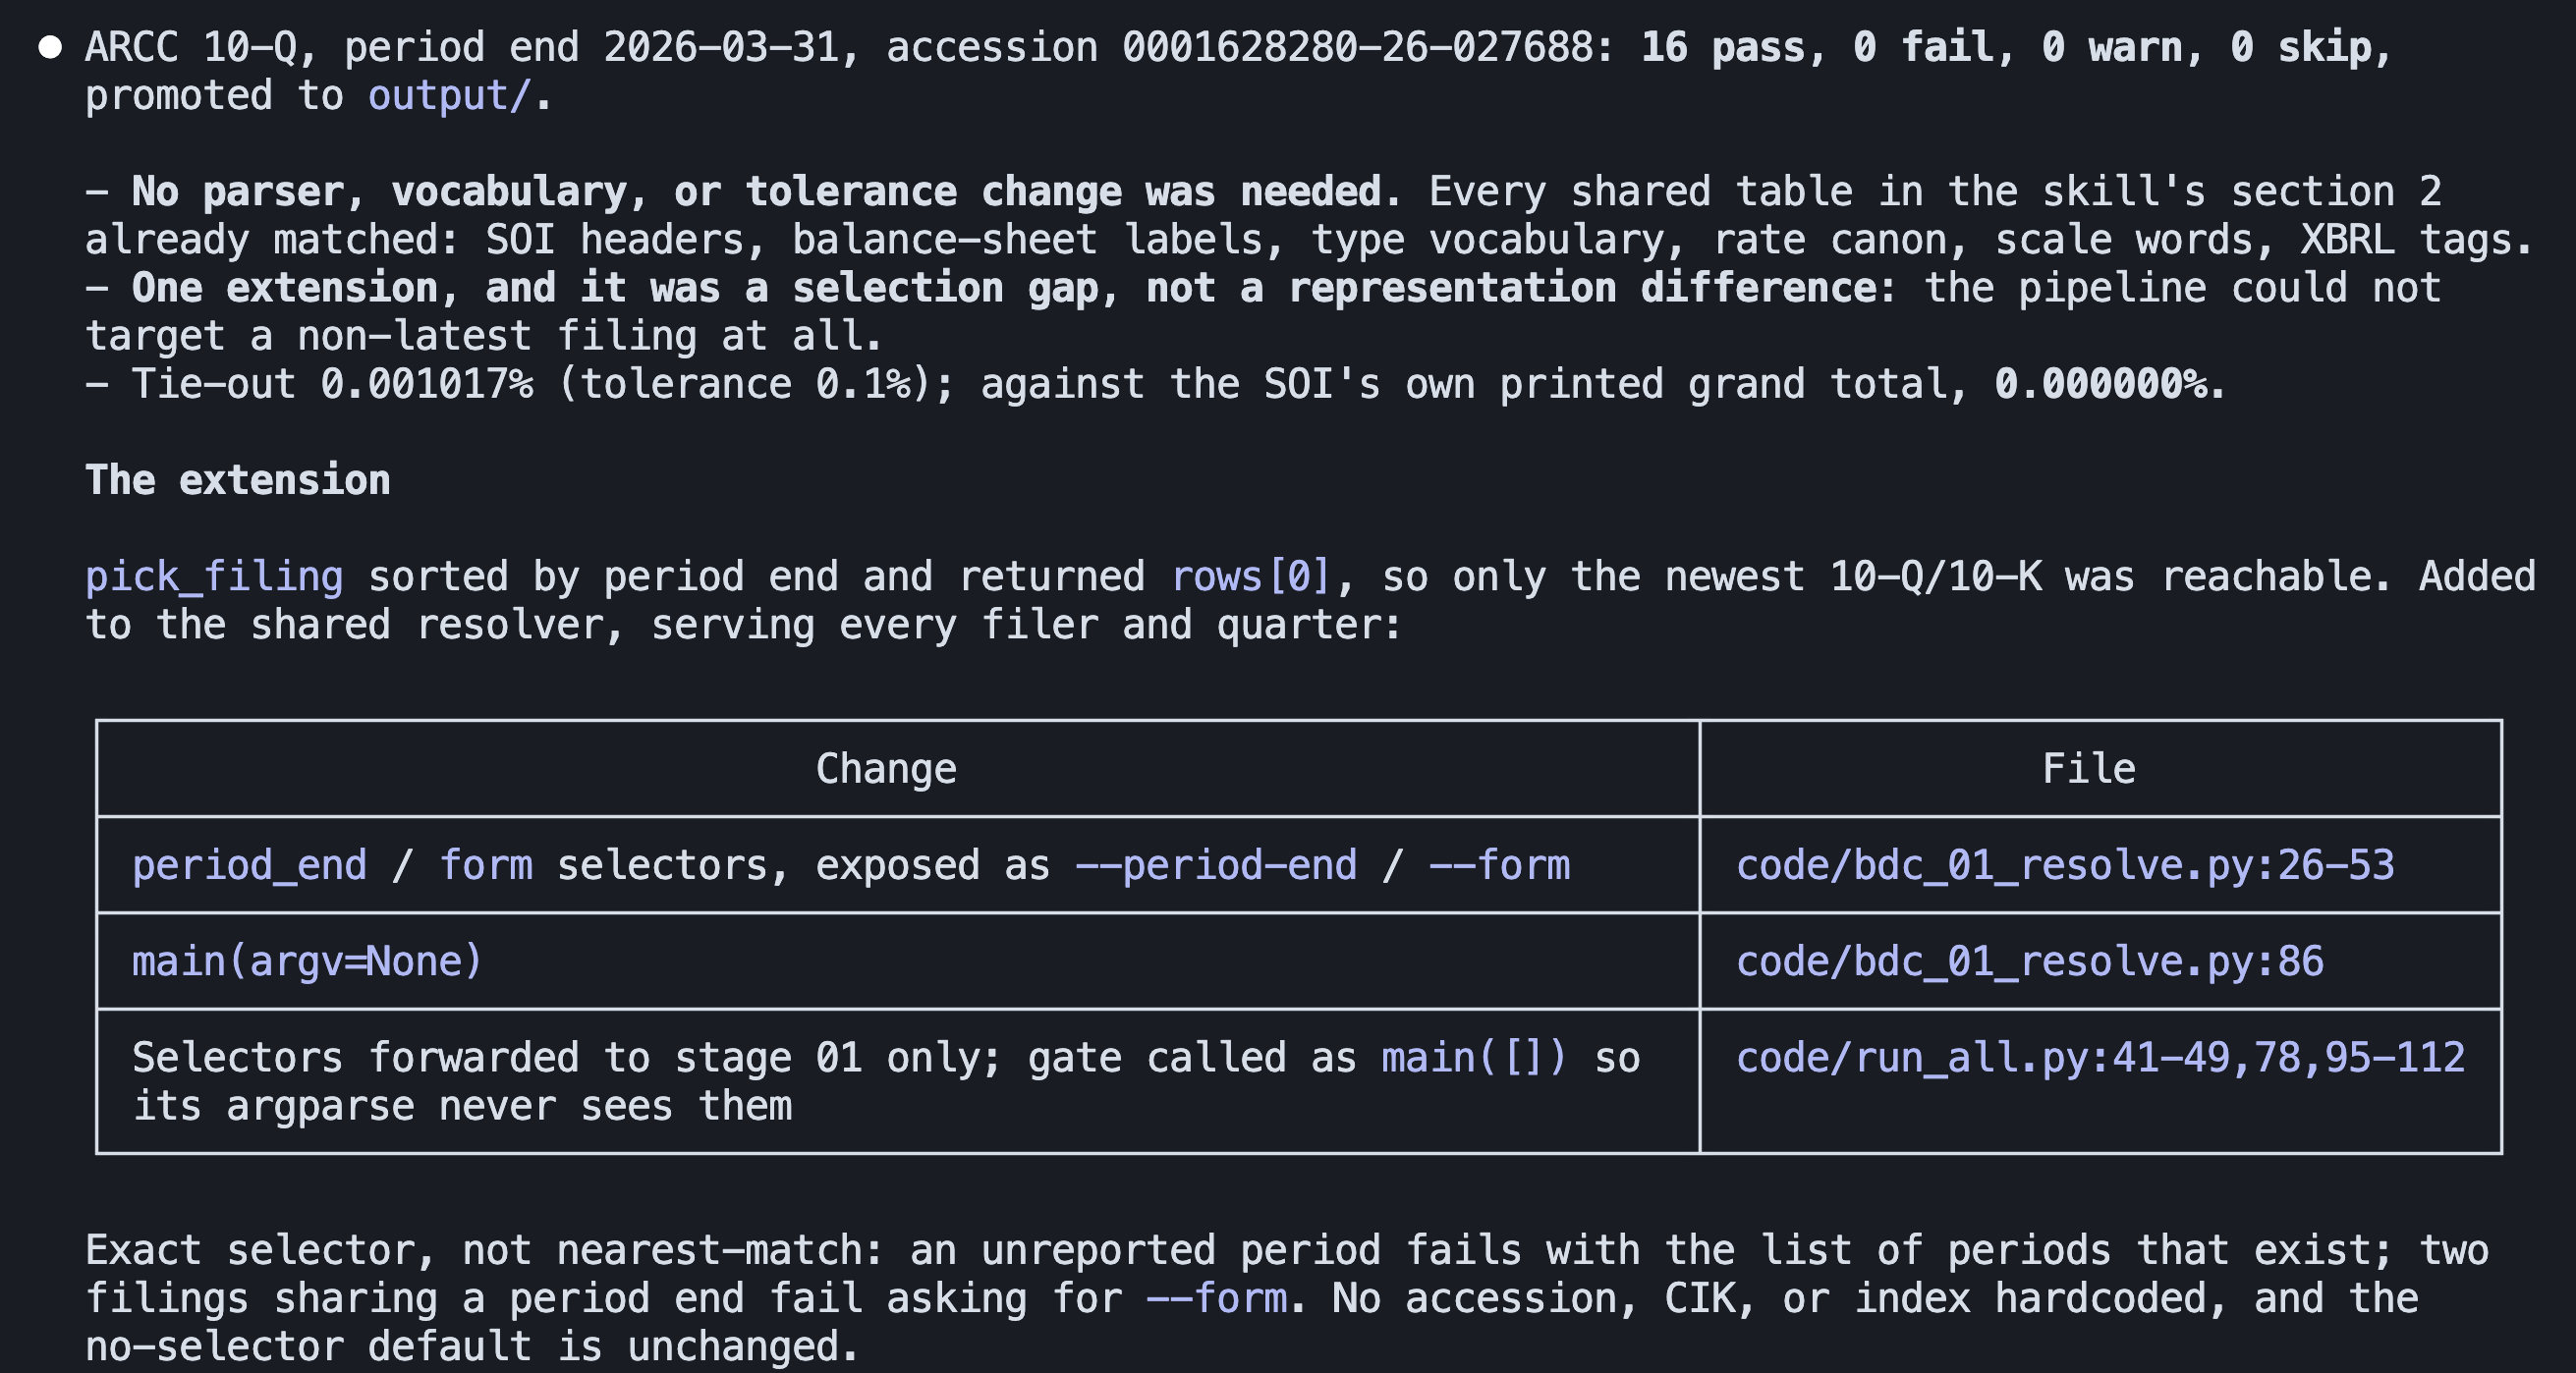
\includegraphics[width=0.8\textwidth]{bdc_design_pharse2-6.png}
\end{center}
\end{frame}

% Sweep every filing. Coverage table and what stopped it.
\begin{frame}[fragile]{Prompt: parameterize, then sweep}
\begin{prompt}[basicstyle=\scriptsize\ttfamily\color{white}]
/bdc-soi-parse every 10-K and 10-Q ARCC has filed with a period end on or after 2023-01-01. Work oldest to newest so failures cluster visibly.
Then assemble all successful filings into a single BDC-quarter panel and check that (cik, period_end) is unique. Report what you find before fixing it.
\end{prompt}
\begin{itemize}
    \item I ran it three times; each time it found new failures and fixed some of them.
    \item Pipeline grew 2,757 to 4,009 lines (+45\%); \file{trap\_log.md} reached 491 lines.
    \item 37,197 positions; \ybb{30 of 34} from 2018 onward; \ybb{14 of 14} from 2023 onward.
\end{itemize}

\begin{center}
\tabfont
\begin{tabular}{lll}
\toprule
Pass & In panel & Note \\
\midrule
Baseline (step 1 parser, unchanged) & 5 of 88 & \\
After first sweep and repair & 22 of 88 & Went backwards in time, oldest first \\
After another pass, asking it to try again & 43 of 88 & Reached 2005; the recent hole untouched \\
Focused on post-2018, newest first & \ybb{50 of 88} & The recent hole closed \\
\bottomrule
\end{tabular}
\end{center}
\end{frame}

% Closing: what you already trust must not move.
\begin{frame}{What you already trust must not move}
\begin{center}\tabfont
\begin{tabular}{lrr}
\toprule
Reference filing, 2026-06-30 & After step 1 & After step 2 \\
\midrule
Positions & 1,439 & 1,439 \\
Distinct borrowers & 593 & 593 \\
Sum of fair value (USD) & 29,349,300,000 & 29,349,300,000 \\
\bottomrule
\end{tabular}
\end{center}
\vs
\begin{wideitemize}
    \item Byte-identical through \ybb{45 filings} of edits. 
    \item It kept a saved copy and diffed after every change.
    \item It also recorded a bug it \ybb{introduced} during the backfill.
\end{wideitemize}
\vs
\takeaway{When you extend a model, make sure the thing you already trust does not move.}
\end{frame}

% Step 3: analysis and report. 9 frames, hands-on, session 1:45-2:08.
\section{Step 3. Analysis and report}\subsection{}

% Step 3 opener. Step table, this row tinted.
\begin{frame}{Step 3. Analysis and report}
\begin{center}
\tabfont
\begin{tabular}{cll}
\toprule
Step & What we build & The concept it forces \\
\midrule
0 & Naive baseline: one prompt & A passing check is only as good as its \ybb{scope} \\
1 & Write a spec, then build & \ybb{Plan mode}, \ybb{sub-agents} for independent verification \\
2 & Generalize across quarters & \ybb{Skills}, and the tie-out as a test suite \\
\rowcolor{yo!10}\yob{3} & \yob{Analysis and report} & \yob{Analysis as verification; grounding in your references} \\
\bottomrule
\end{tabular}
\end{center}

\vs
\begin{itemize}
    \item After Step 2, we have a panel ready for analysis.
    \item One prompt to analyze the panel and produce a report.
    \item And using the data turns out to be \ybb{a check of its own}.
\end{itemize}
\end{frame}

% The prompt, verbatim. One turn, no follow-ups.
\begin{frame}[fragile]{\yob{LAB: }The prompt}
\begin{prompt}[basicstyle=\scriptsize\ttfamily\color{white}]
ultracode
Based on the 2018-2026 data in output/panel/bdc_quarter.csv and output/panel/bdc_quarter_investment.csv, produce an industry report on this portfolio. Write the code to analysis and output everything to output/analysis. The analysis report style follows the documents in reference, and should be in both .docx and .pdf, with figures and tables. It should at least include sample coverage, summary statistics, time series, deal terms, and cross-section. Be specific about percentages and periods. Every figure and table states the period it covers and the share of rows it is computed on.
\end{prompt}
\end{frame}

% Ultracode, 1 of 2.
\begin{frame}{Ultracode}
\begin{itemize}
    \item \yob{Ultracode} is dynamic workflows orchestrate many subagents, skills, and tools, so that it can plan and execute complex tasks.
    \item Same mechanism as the sub-agents in step 1, at a larger scale and scheduled by the tool rather than by me.
\end{itemize}
\begin{center}
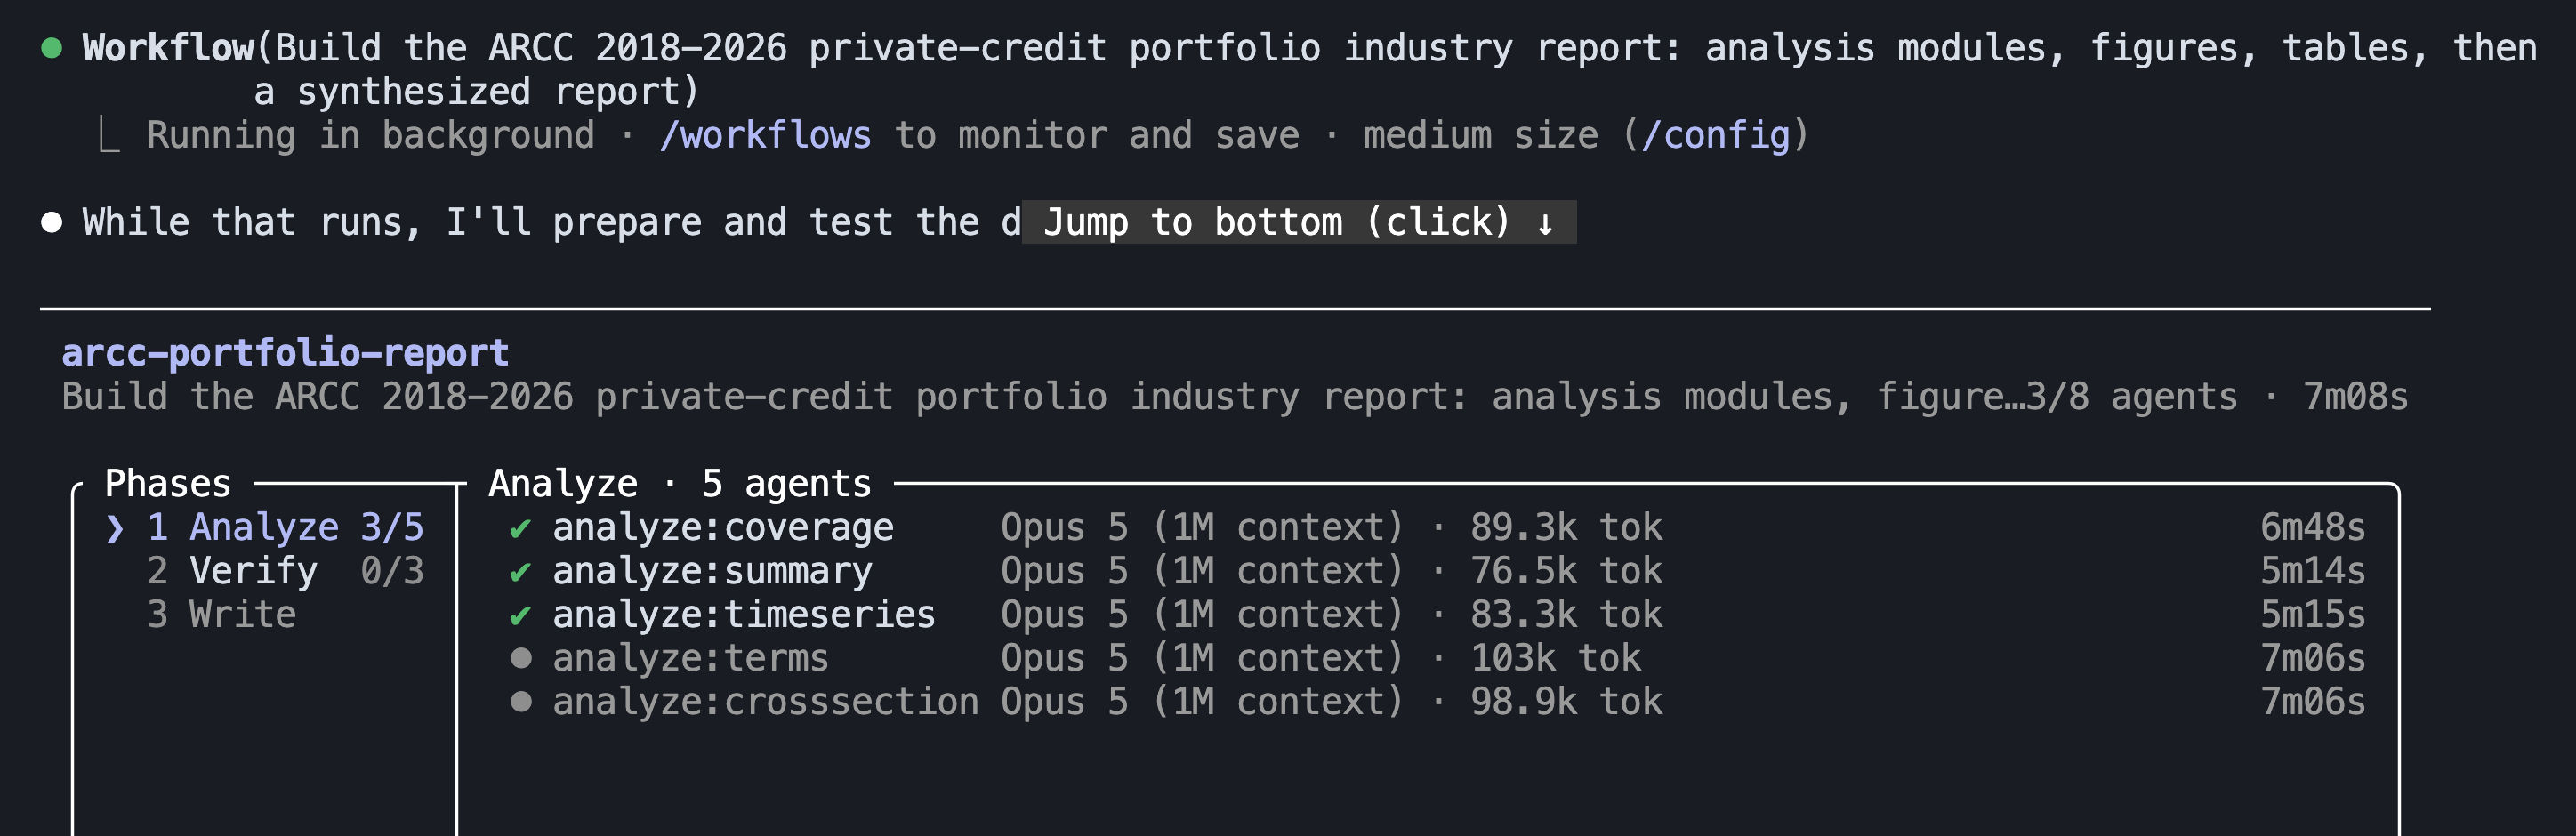
\includegraphics[width=1\textwidth]{bdc_design_pharse3-2.png}
\end{center}
\end{frame}

% Ultracode, 2 of 2.
\begin{frame}{Ultracode}
\begin{itemize}
    \item \yob{Ultracode} is dynamic workflows orchestrate many subagents, skills, and tools, so that it can plan and execute complex tasks.
    \item Same mechanism as the sub-agents in step 1, at a larger scale and scheduled by the tool rather than by me.
\end{itemize}
\begin{center}
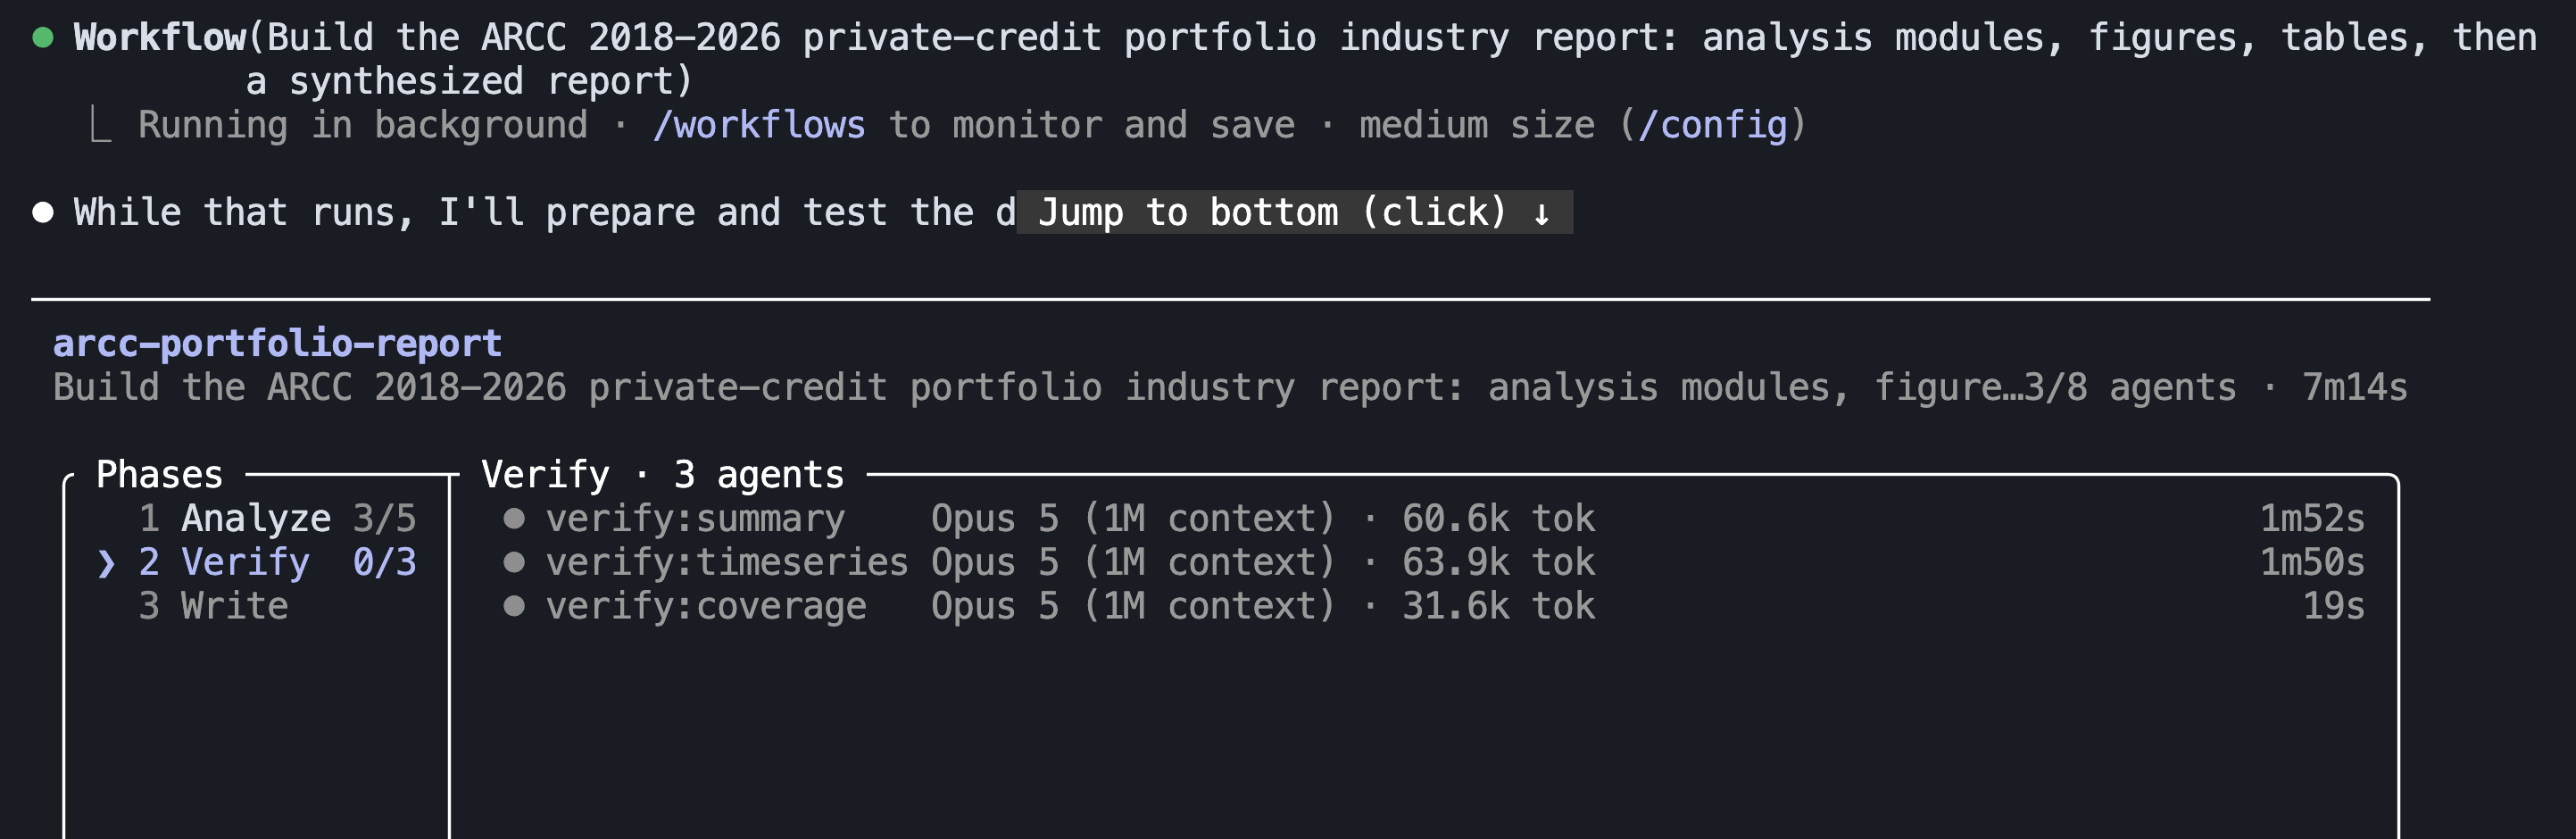
\includegraphics[width=1\textwidth]{bdc_design_pharse3-3.png}
\end{center}
\end{frame}

% Grounding: the style comes from documents you supply.
\begin{frame}{Style in \file{reference/}}
\begin{itemize}
    \item Prompt: \ylbb{``the analysis report style follows the
        documents in reference''}.
    \item We want to control the style and format of the report. It can look like an industry report, or an academic paper. But we don't want to type every detail by hand. 
    \item \file{reference/} holds three industry report PDFs I downloaded.
    \item \ylbb{What transferred:} exhibit numbering, a source line under every
        exhibit, a ``Finding.'' sentence opening each section, a limitations section.
\end{itemize}
\ybb{Further usage}
\begin{itemize}
  \item \ylbb{Build an index} once the corpus is too big to attach every time:
        queried rather than pasted, and reusable. Part 4.
  \item \ylbb{Turn your own style into a skill}, so the next report starts from
        your conventions.
\end{itemize}
\end{frame}

% One prompt, 53 pages.
\begin{frame}{One prompt, 53 pages}
\begin{center}
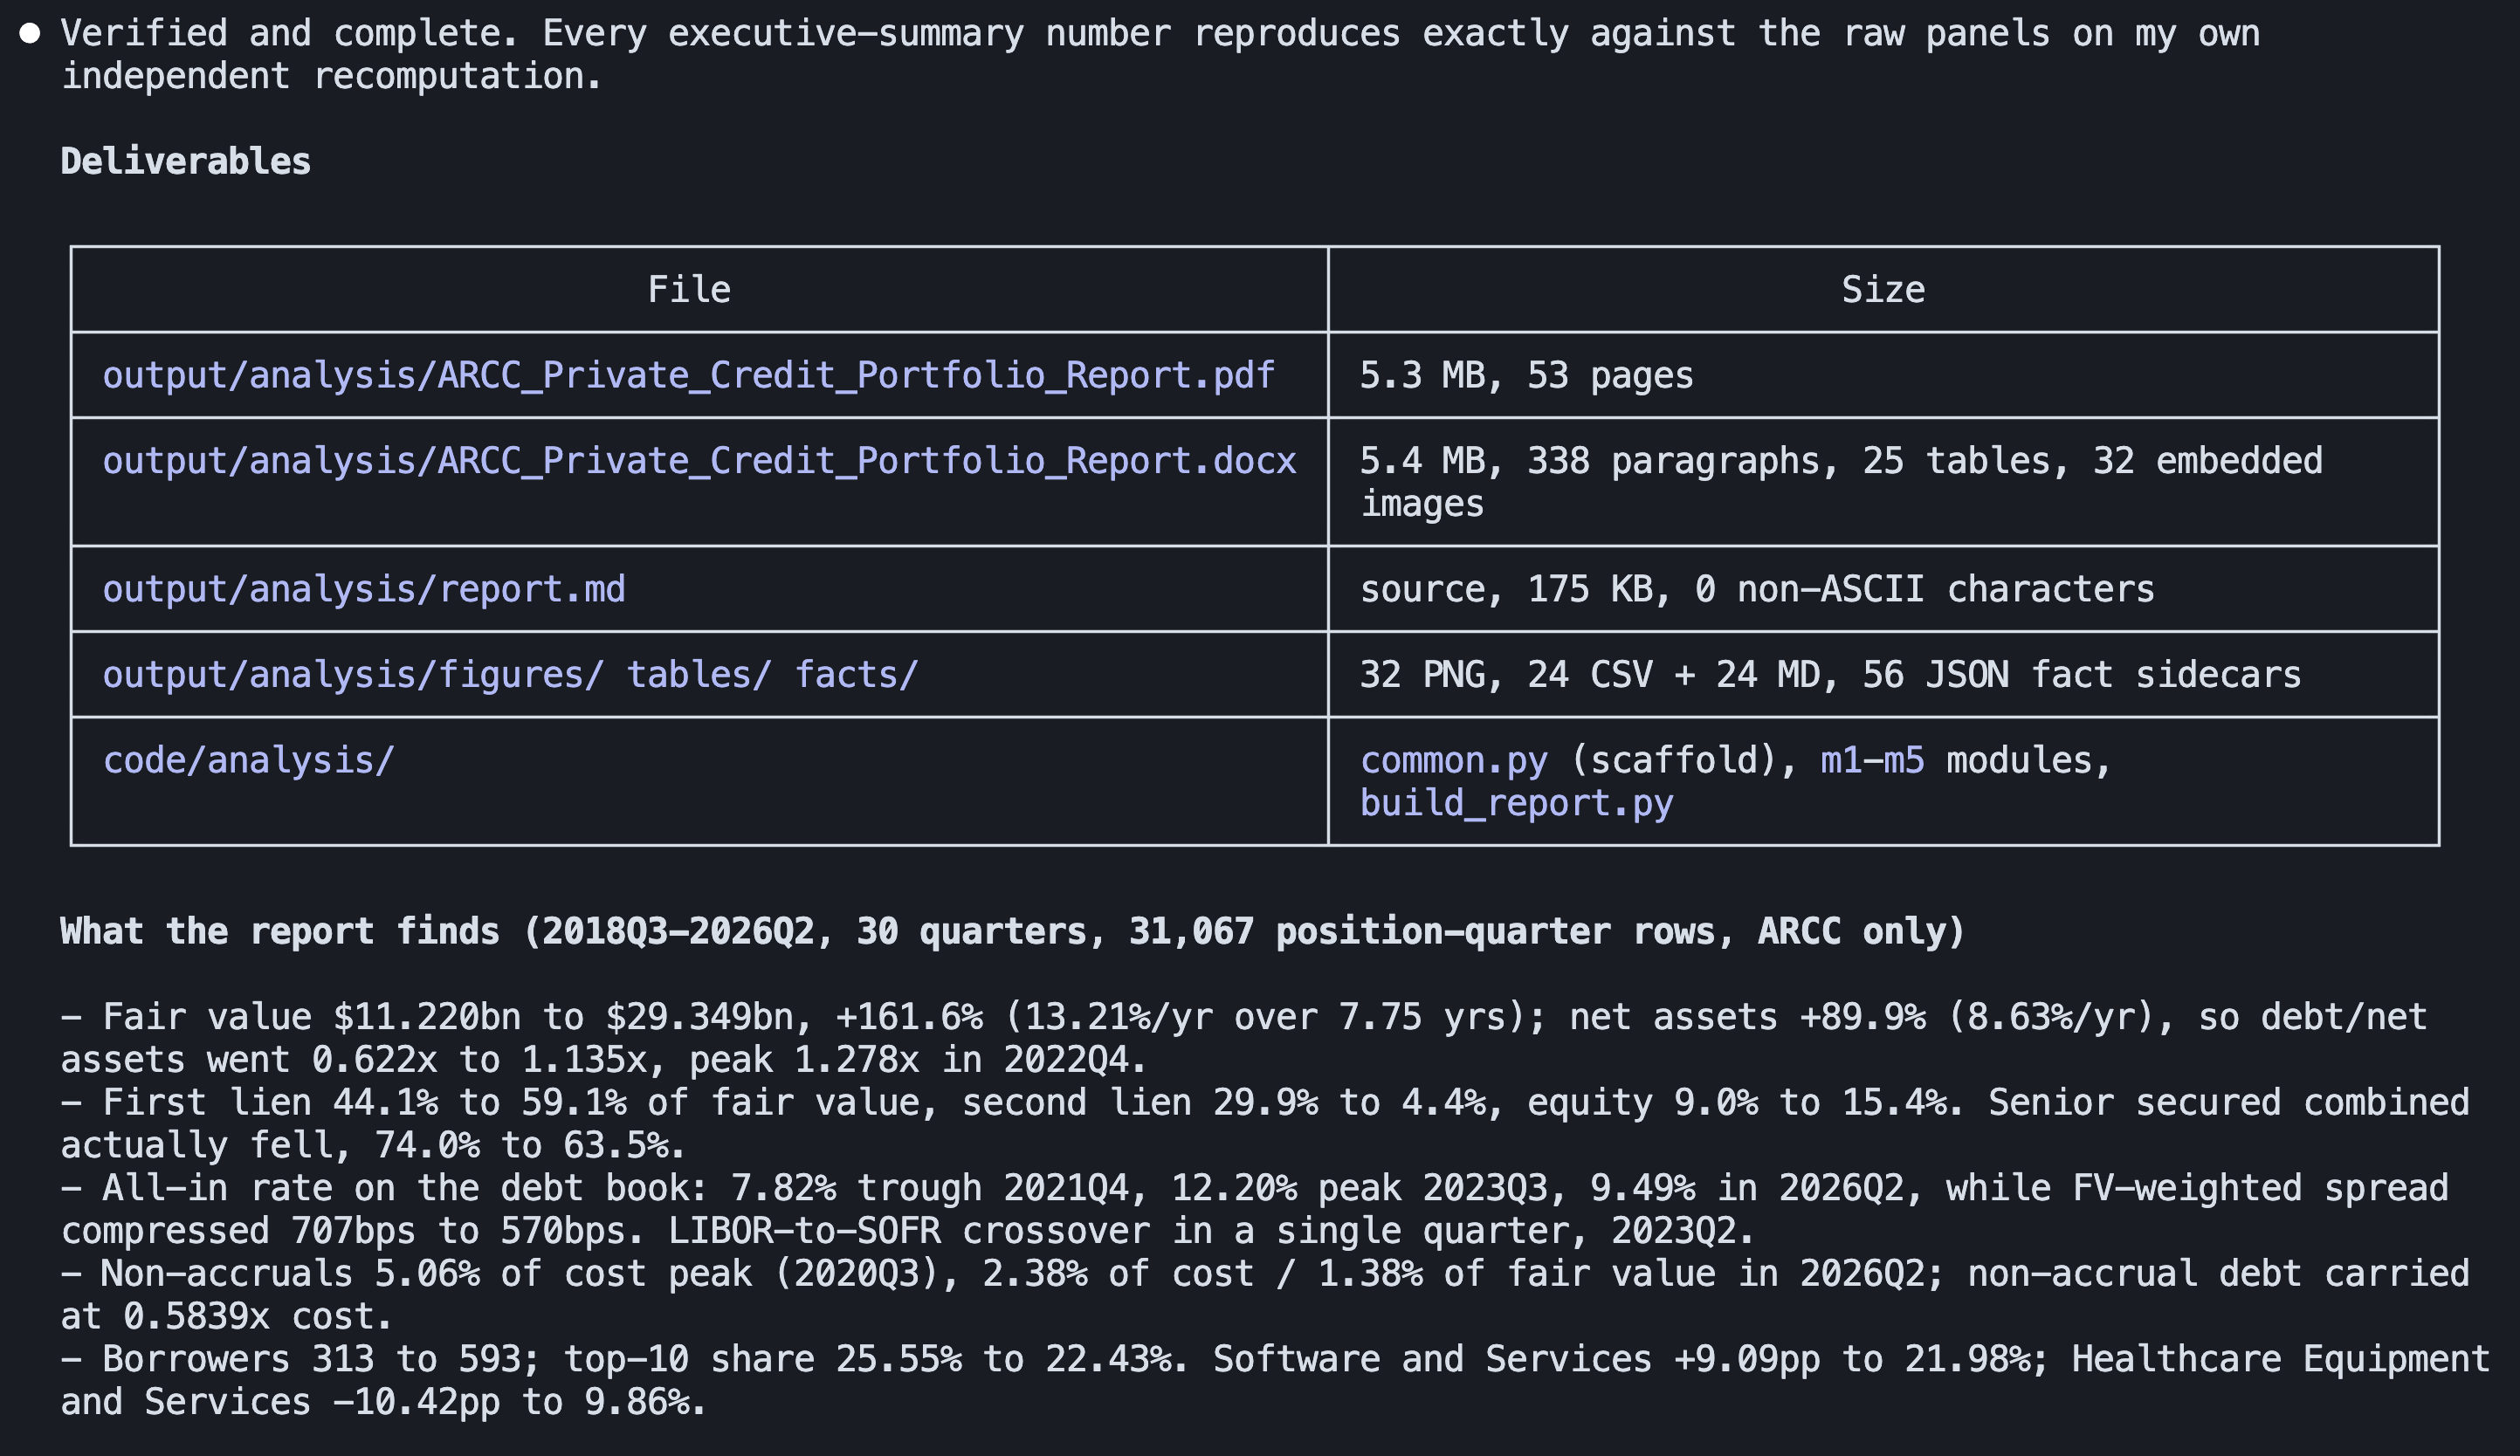
\includegraphics[width=0.7\textwidth]{bdc_design_pharse3-4.png}
\end{center}
\vspace{-0.5cm}
\begin{itemize}
    \item Report: 53 pages, 21,006 words, 32 figures and 48 tables.
    \item Analysis is not the cheap part: 4,086 lines of code. The previous pipeline: 4,009 lines.
\end{itemize}
\end{frame}

% The report itself.
\begin{frame}{The report}
\begin{columns}
\begin{column}{0.5\textwidth}
\begin{center}
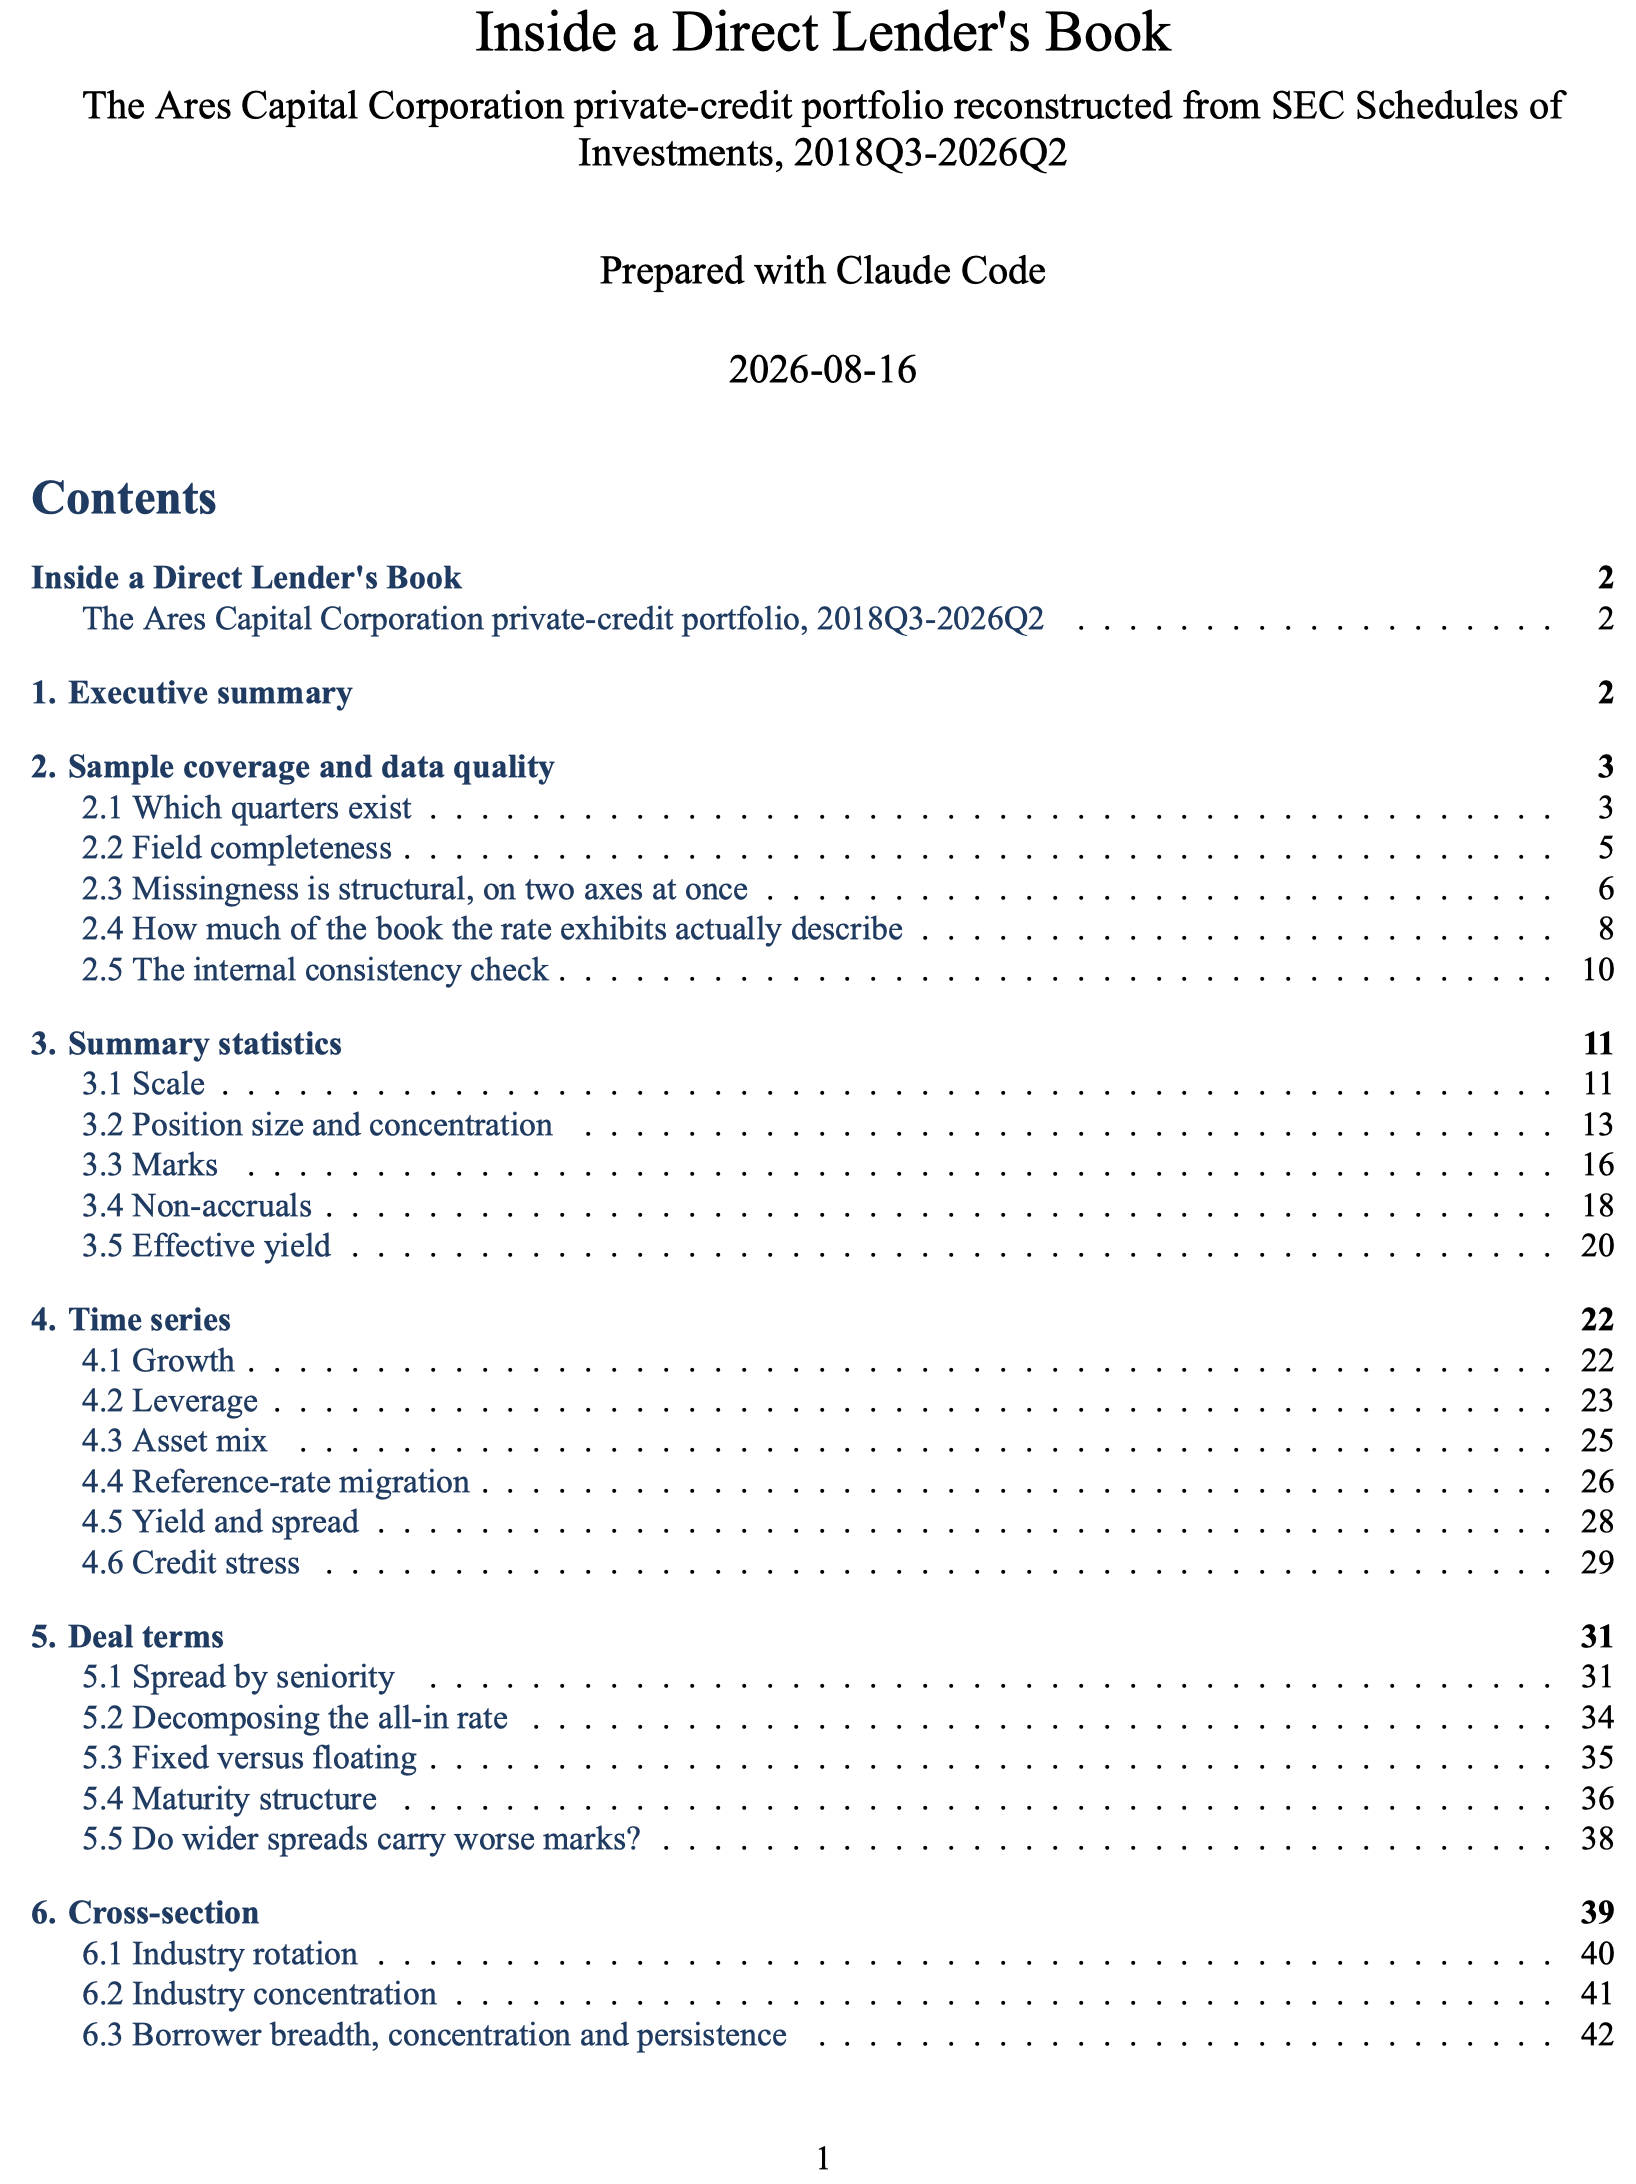
\includegraphics[width=0.8\textwidth]{bdc_design_pharse3_report.png}
\end{center}
\end{column}
\begin{column}{0.5\textwidth}
\begin{itemize}
  \item Eight sections, among them: executive summary, coverage, summary statistics,
        time series, deal terms, cross-section, limitations.
  \item Every exhibit carries \ybb{its period and its coverage}, because the prompt
        said so and the code enforced it.
\end{itemize}
\end{column}
\end{columns}
\end{frame}

% Example exhibit: balance-sheet growth over time.
\begin{frame}{Example exhibit: the time series of balance sheet growth}
\begin{center}
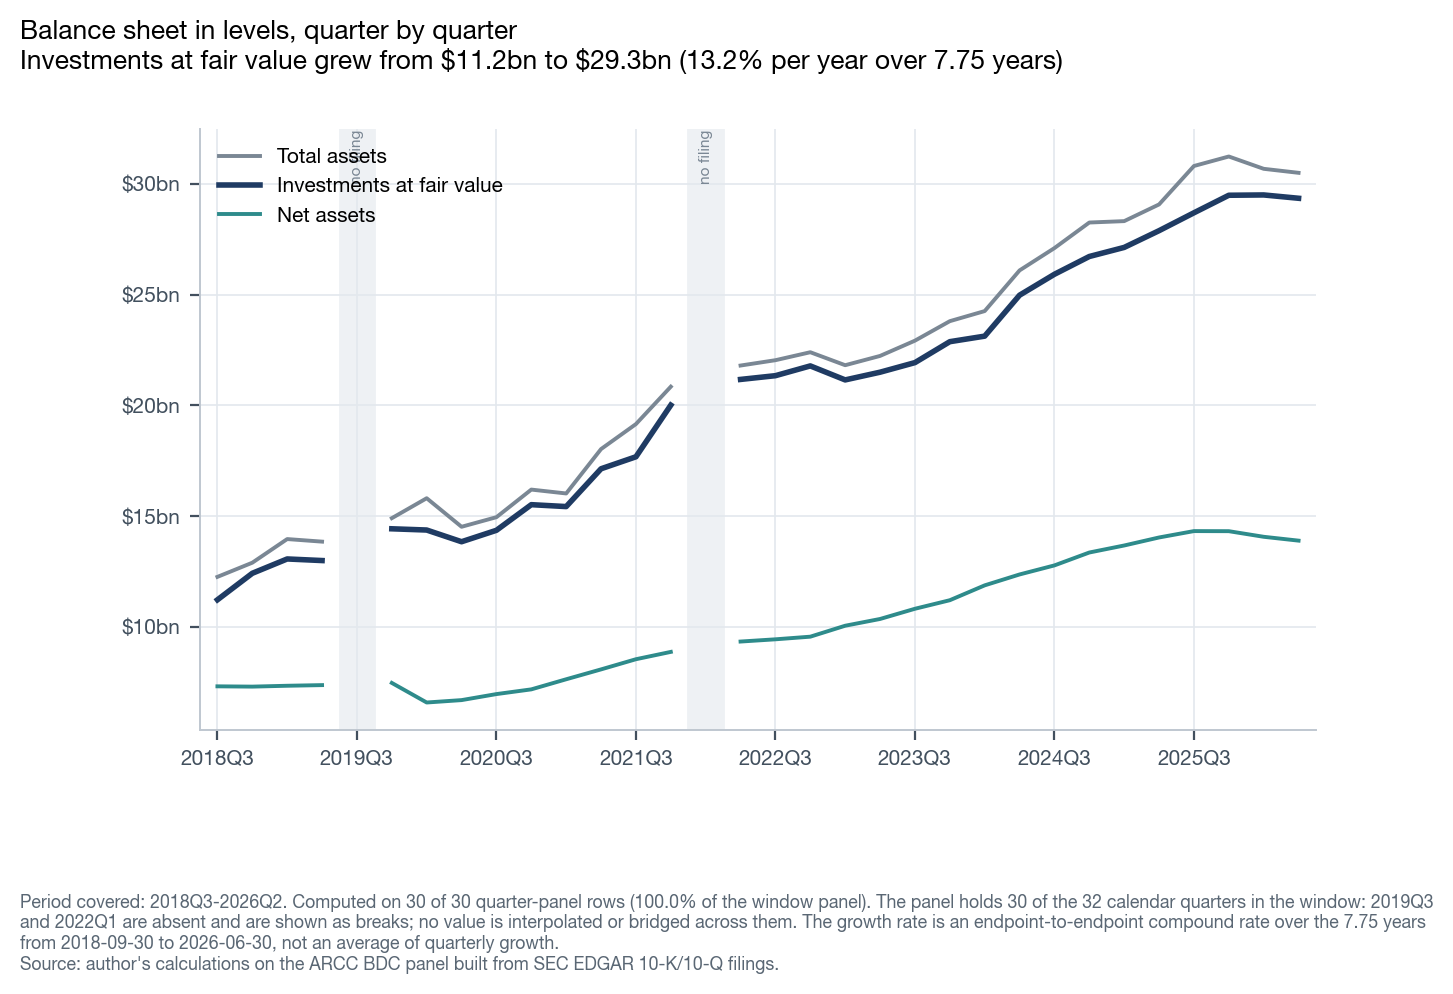
\includegraphics[width=0.8\textwidth]{ts_growth_levels.png}
\end{center}
\end{frame}

% The payoff: the analysis found a bug sixteen checks passed over.
\begin{frame}{The analysis found a bug that previous checks passed over}
\vs
The report, in its own section 4.6, \ybb{unprompted}:
\begin{quote}
``The non-accrual series is drawn on 27 of the 30 quarters: 2022Q4, 2023Q4 and
2024Q4 return exactly zero parsed flags while neighbouring quarters carry 13 to
22, which is a \yob{footnote-marker parse failure and not a clean book}.''
\end{quote}
\vspace{-0.5cm}
\begin{itemize}\small
  \item \ybb{Why no check saw it.} \file{is\_non\_accrual} is a boolean, so
        \yob{no tie-out reaches it} -- and the column is 0.00\% null: fully
        populated, and in three quarters uniformly wrong.
\end{itemize}
\takeaway{Analysis can be viewed as another verification layer.}
\end{frame}


%=======================================================================
%                              PART 3
%=======================================================================
% Part 3: more useful concepts. Divider plus 3 frames, session 2:08-2:36.
\section{Part 3. More useful concepts}\subsection{}

% Part 3 divider.
\begin{transitionframe}
Part 3. More useful concepts
\end{transitionframe}

% The eight working tips, as one list.
\begin{frame}{Working tips}
\begin{enumerate}
    \item Plan before acting.
    \item Be specific.
    \item Always have a backup.
    \item Manage your context window.
    \item Always have a way to verify outputs.
    \item Ask the LLM to take notes.
    \item Be replicable.
    \item Stay organized with your code, data, and notes.
\end{enumerate}
\end{frame}

% Permissions, honestly.
\begin{frame}{AI safety: honestly, you will grant most permissions}
\begin{wideitemize}
    \item Every step today asked for file writes, shell access and network access. It is unrealistic to approve every single permission every time.
    \item The best you can do is to allow-list broadly and stop reading.
    \item Which is tip 3 again, for a different reason: \ybb{always have a backup.}
    \item Mine is GitHub for code and Dropbox for data, and my own agents run on \ybb{a separate Mac Mini} -- a machine with limited access to my data that I can wipe.
    \item The real question is not ``what may it do'' but \yob{``what can it reach''}.
\end{wideitemize}
\end{frame}

% Dev containers: what isolation buys and what it does not.
\begin{frame}{Dev containers are the real alternative}
\begin{wideitemize}
    \item Cost: Docker, a config file, and a slower first run. Windows needs WSL2.
    \item Isolation is about \ybb{what is reachable}. 
    \item See ``\#7 Permissions, Sandboxes, and Autonomous Agents'' in \emph{A Series on Claude Code}, by Paul Goldsmith-Pinkham.
\end{wideitemize}
\end{frame}


%=======================================================================
%                              PART 4
%=======================================================================
% Part 4: advanced usage examples. Divider plus 10 frames, session 3:40-3:55.
\section{Part 4. Advanced usage examples}\subsection{}

% Part 4 divider.
\begin{transitionframe}
Part 4. Advanced usage examples
\end{transitionframe}

% Framing: each demo adds an axis Part 2 could not show.
\begin{frame}{Each of these adds something the project could not show}
\begin{center}
\tabfont
\begin{tabular}{lll}
\toprule
Demo & Axis it adds & Where Part 2 stopped \\
\midrule
TravelTab + PetTab & The pipeline becomes \emph{software} & We shipped a report, not a system \\
GBrain    & Retrieval that is \emph{indexed} & Step 3 attached sample docs by hand \\
NanoClaw  & The agent has an \emph{address}  & You were always at the terminal \\
\bottomrule
\end{tabular}
\end{center}
\vs
Nothing here is a new tool. It is the same agent, moved one step along one axis.
\end{frame}

% TravelTab, 1 of 3: the background, as an annoyance.
\begin{frame}{TravelTab: personal-database management}
\begin{wideitemize}
  \item Background: I travel between New Haven and Philadelphia constantly, and Amtrak is
        the only workable way to do it. The app is painful, it does not talk to my
        calendar, \ybb{the ticket arrives once by email and sometimes it is gone}, and
        the pricing is dynamic.
  \item So I built \ybb{TravelTab}, a personal Amtrak ticket tracker:
  \begin{enumerate}\small
      \item \ylbb{Ingests tickets automatically from my email.}
      \item \ylbb{Exports structured records into a database}: one row per
            passenger per ticket.
      \item \ylbb{Syncs into my calendar}, so a trip is something I can actually
            manage.
      \item \ylbb{Fare watch} that checks prices and alerts me.
  \end{enumerate}
  \item I can access it from anywhere, on any device, with a web browser.
\end{wideitemize}
\end{frame}

% TravelTab, 2 of 3: the tickets dashboard.
\begin{frame}{TravelTab: personal-database management}
\begin{center}
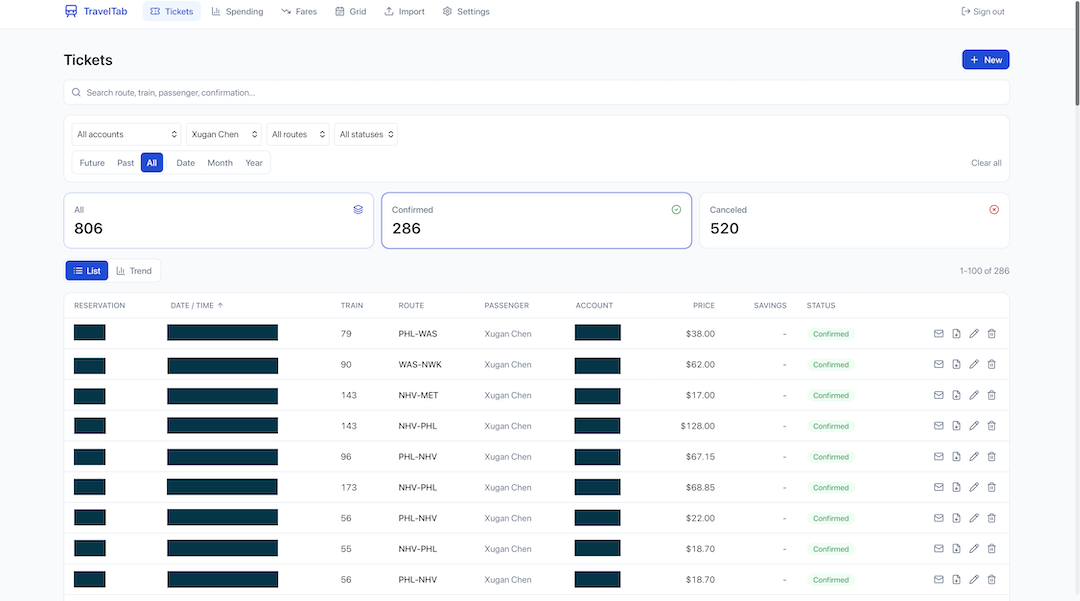
\includegraphics[height=0.8\textheight]{traveltab_tickets1.png}
\end{center}
\vspace{-0.2em}
Every row here arrived as \ybb{an email}. Messy documents in, structured
records out.
\end{frame}

% TravelTab, 3 of 3: the fare watch, which runs unattended.
\begin{frame}{And it keeps running when you are not watching}
\begin{center}
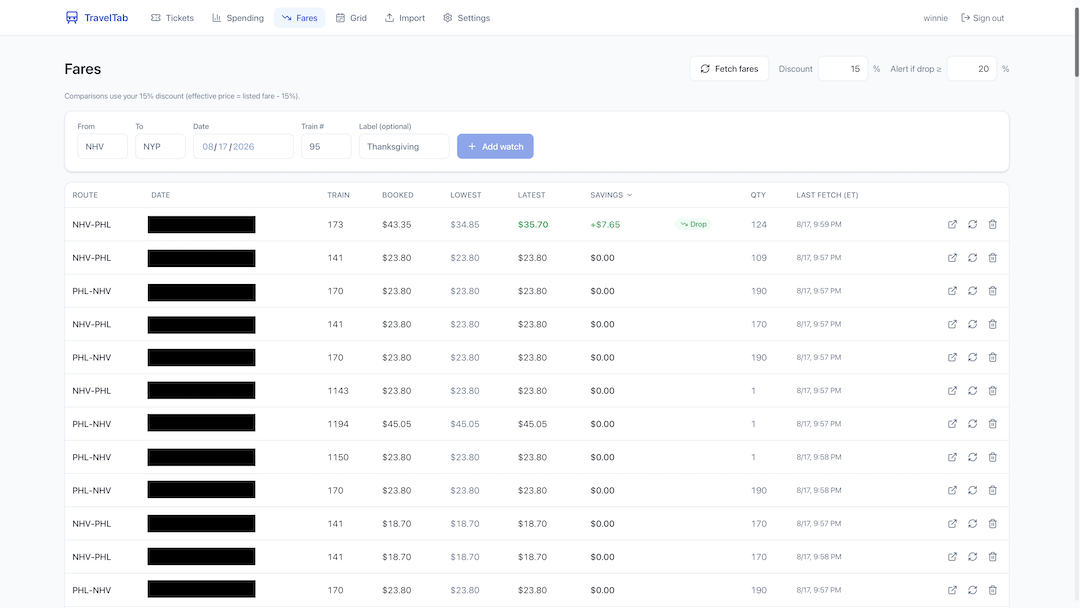
\includegraphics[height=0.8\textheight]{traveltab_fares.png}
\end{center}
\vspace{-0.2em}
\ybb{Fare watchlist} that checks prices on a schedule and alerts me on a threshold.
\end{frame}

% PetTab, 1 of 3: same stack, another domain.
\begin{frame}{PetTab: another domain, same stack}
\begin{columns}[T]
\begin{column}{0.5\textwidth}
\begin{center}

\includegraphics[height=0.5\textheight]{petab_winnie.jpeg}
\end{center}
\end{column}
\begin{column}{0.5\textwidth}
\begin{center}

\includegraphics[height=0.5\textheight]{petab_dory.jpg}
\end{center}
\end{column}
\end{columns}
\vs
\begin{itemize}
    \item Background: I have two cats, Winnie and Dory, and I want to track their health and bahavior. Existing tools are too complicated, and I want full control over the data.
    \item So I built \ybb{PetTab}, a pet-health logger built on TravelTab's stack.
\end{itemize}
\end{frame}

% PetTab, 2 of 3: the data views.
\begin{frame}{PetTab: visualizing the data}
\begin{center}
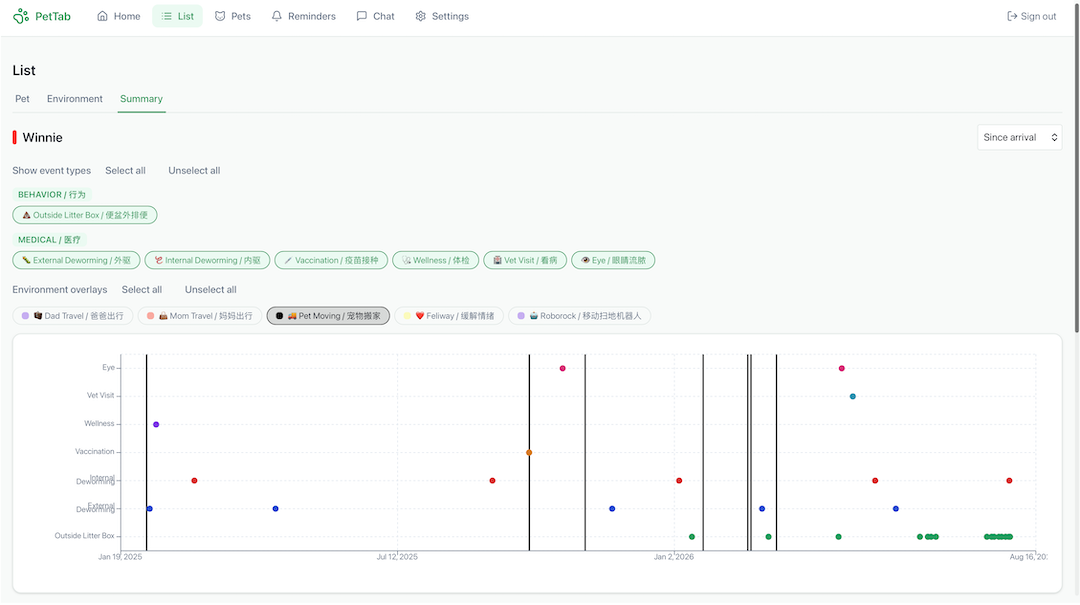
\includegraphics[width=0.9\textwidth]{pettab_list.png}
\end{center}
\end{frame}

% PetTab, 3 of 3: an agent inside the product, on a read-only snapshot.
\begin{frame}{PetTab: a chat agent inside the product}
\begin{columns}[T]
\begin{column}{0.55\textwidth}
\begin{center}
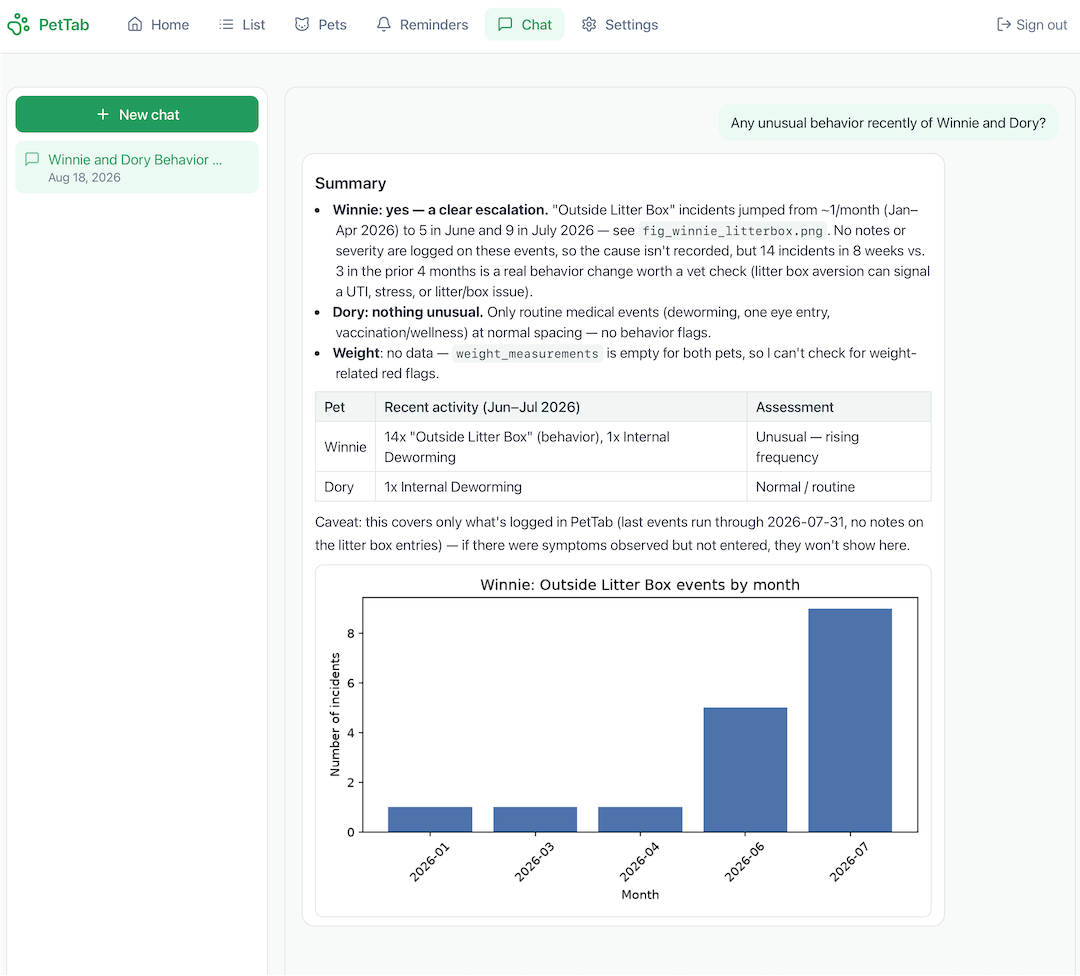
\includegraphics[width=\textwidth]{pettab_chat.png}
\end{center}
\end{column}
\begin{column}{0.45\textwidth}
\vs
\begin{itemize}
    \item An agent is embedded within the product.
    \item PetTab's Insights chat runs the \file{claude} CLI over a
        \ybb{read-only snapshot} of the database, so that it can explore the database and give me suggestions or help me manage the reminders.
\end{itemize}
\end{column}
\end{columns}
\end{frame}

% GBrain: indexed retrieval over a corpus you own.
\begin{frame}{GBrain: personal-knowledge brain}
\begin{columns}[T]
\begin{column}{0.5\textwidth}

\includegraphics[width=\textwidth]{gbrain1.png}
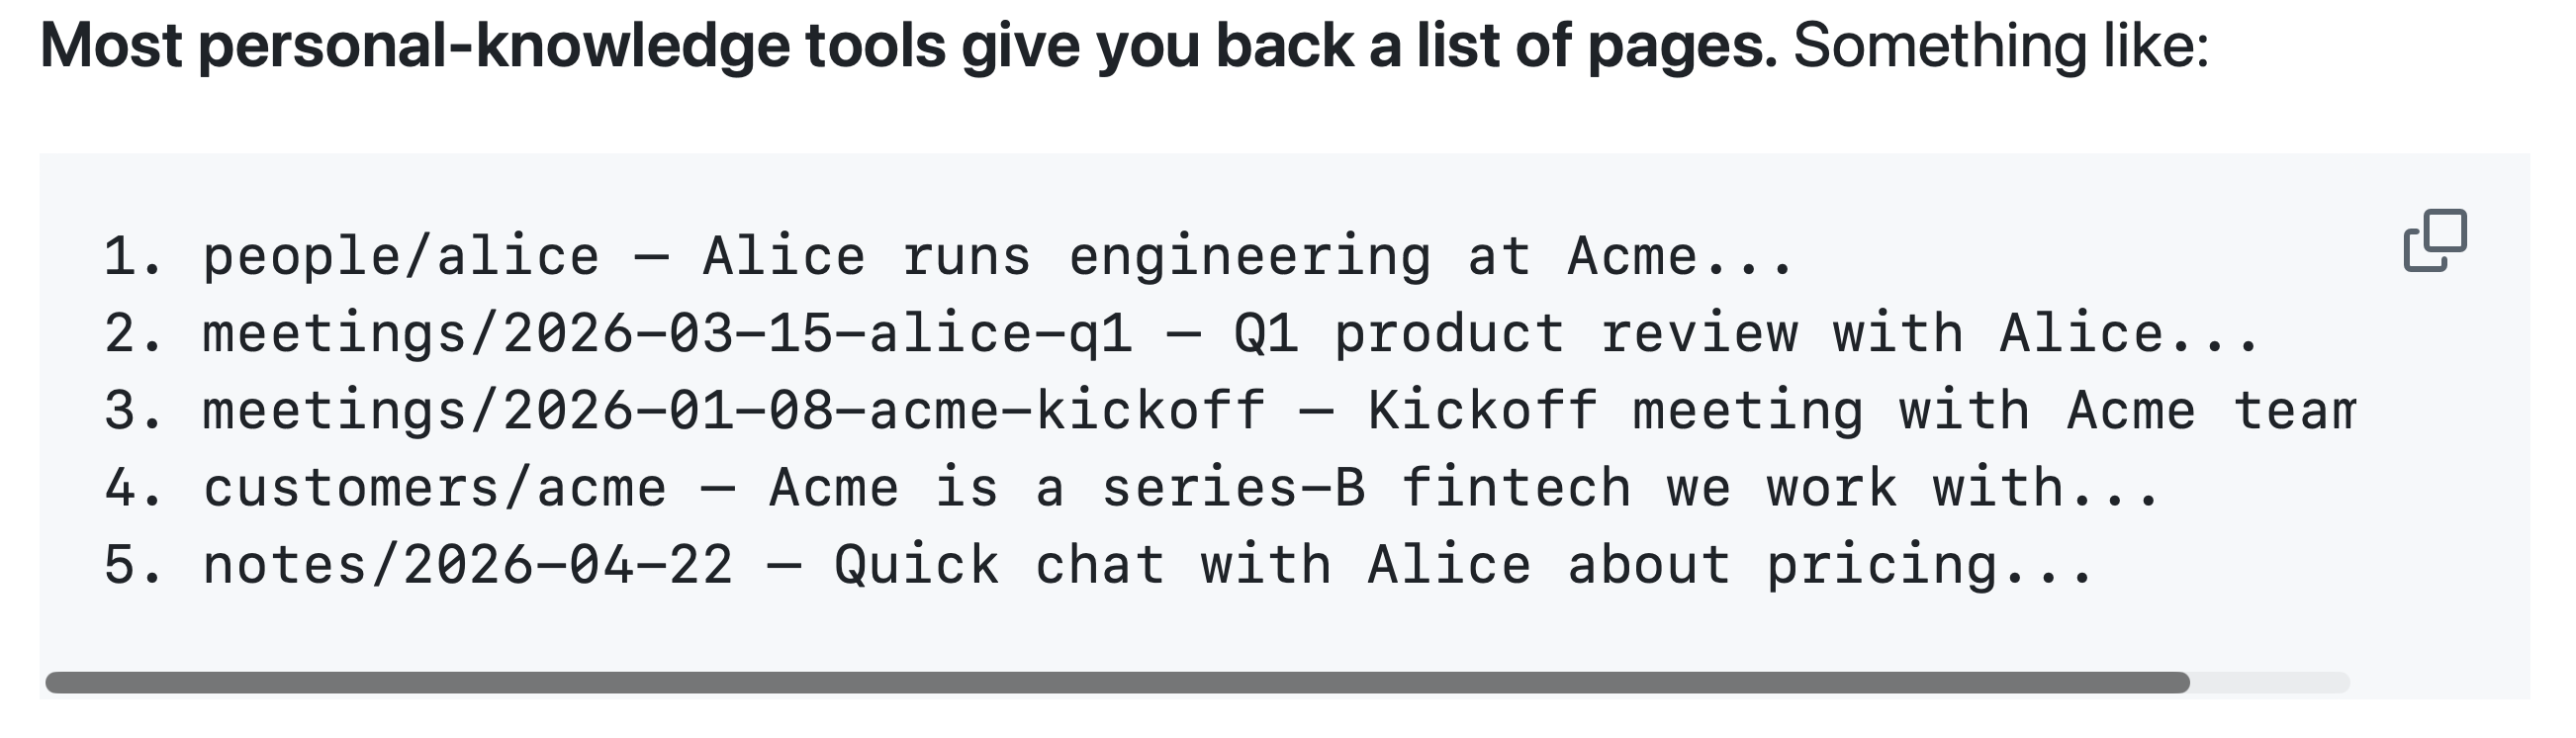
\includegraphics[width=\textwidth]{gbrain2.png}
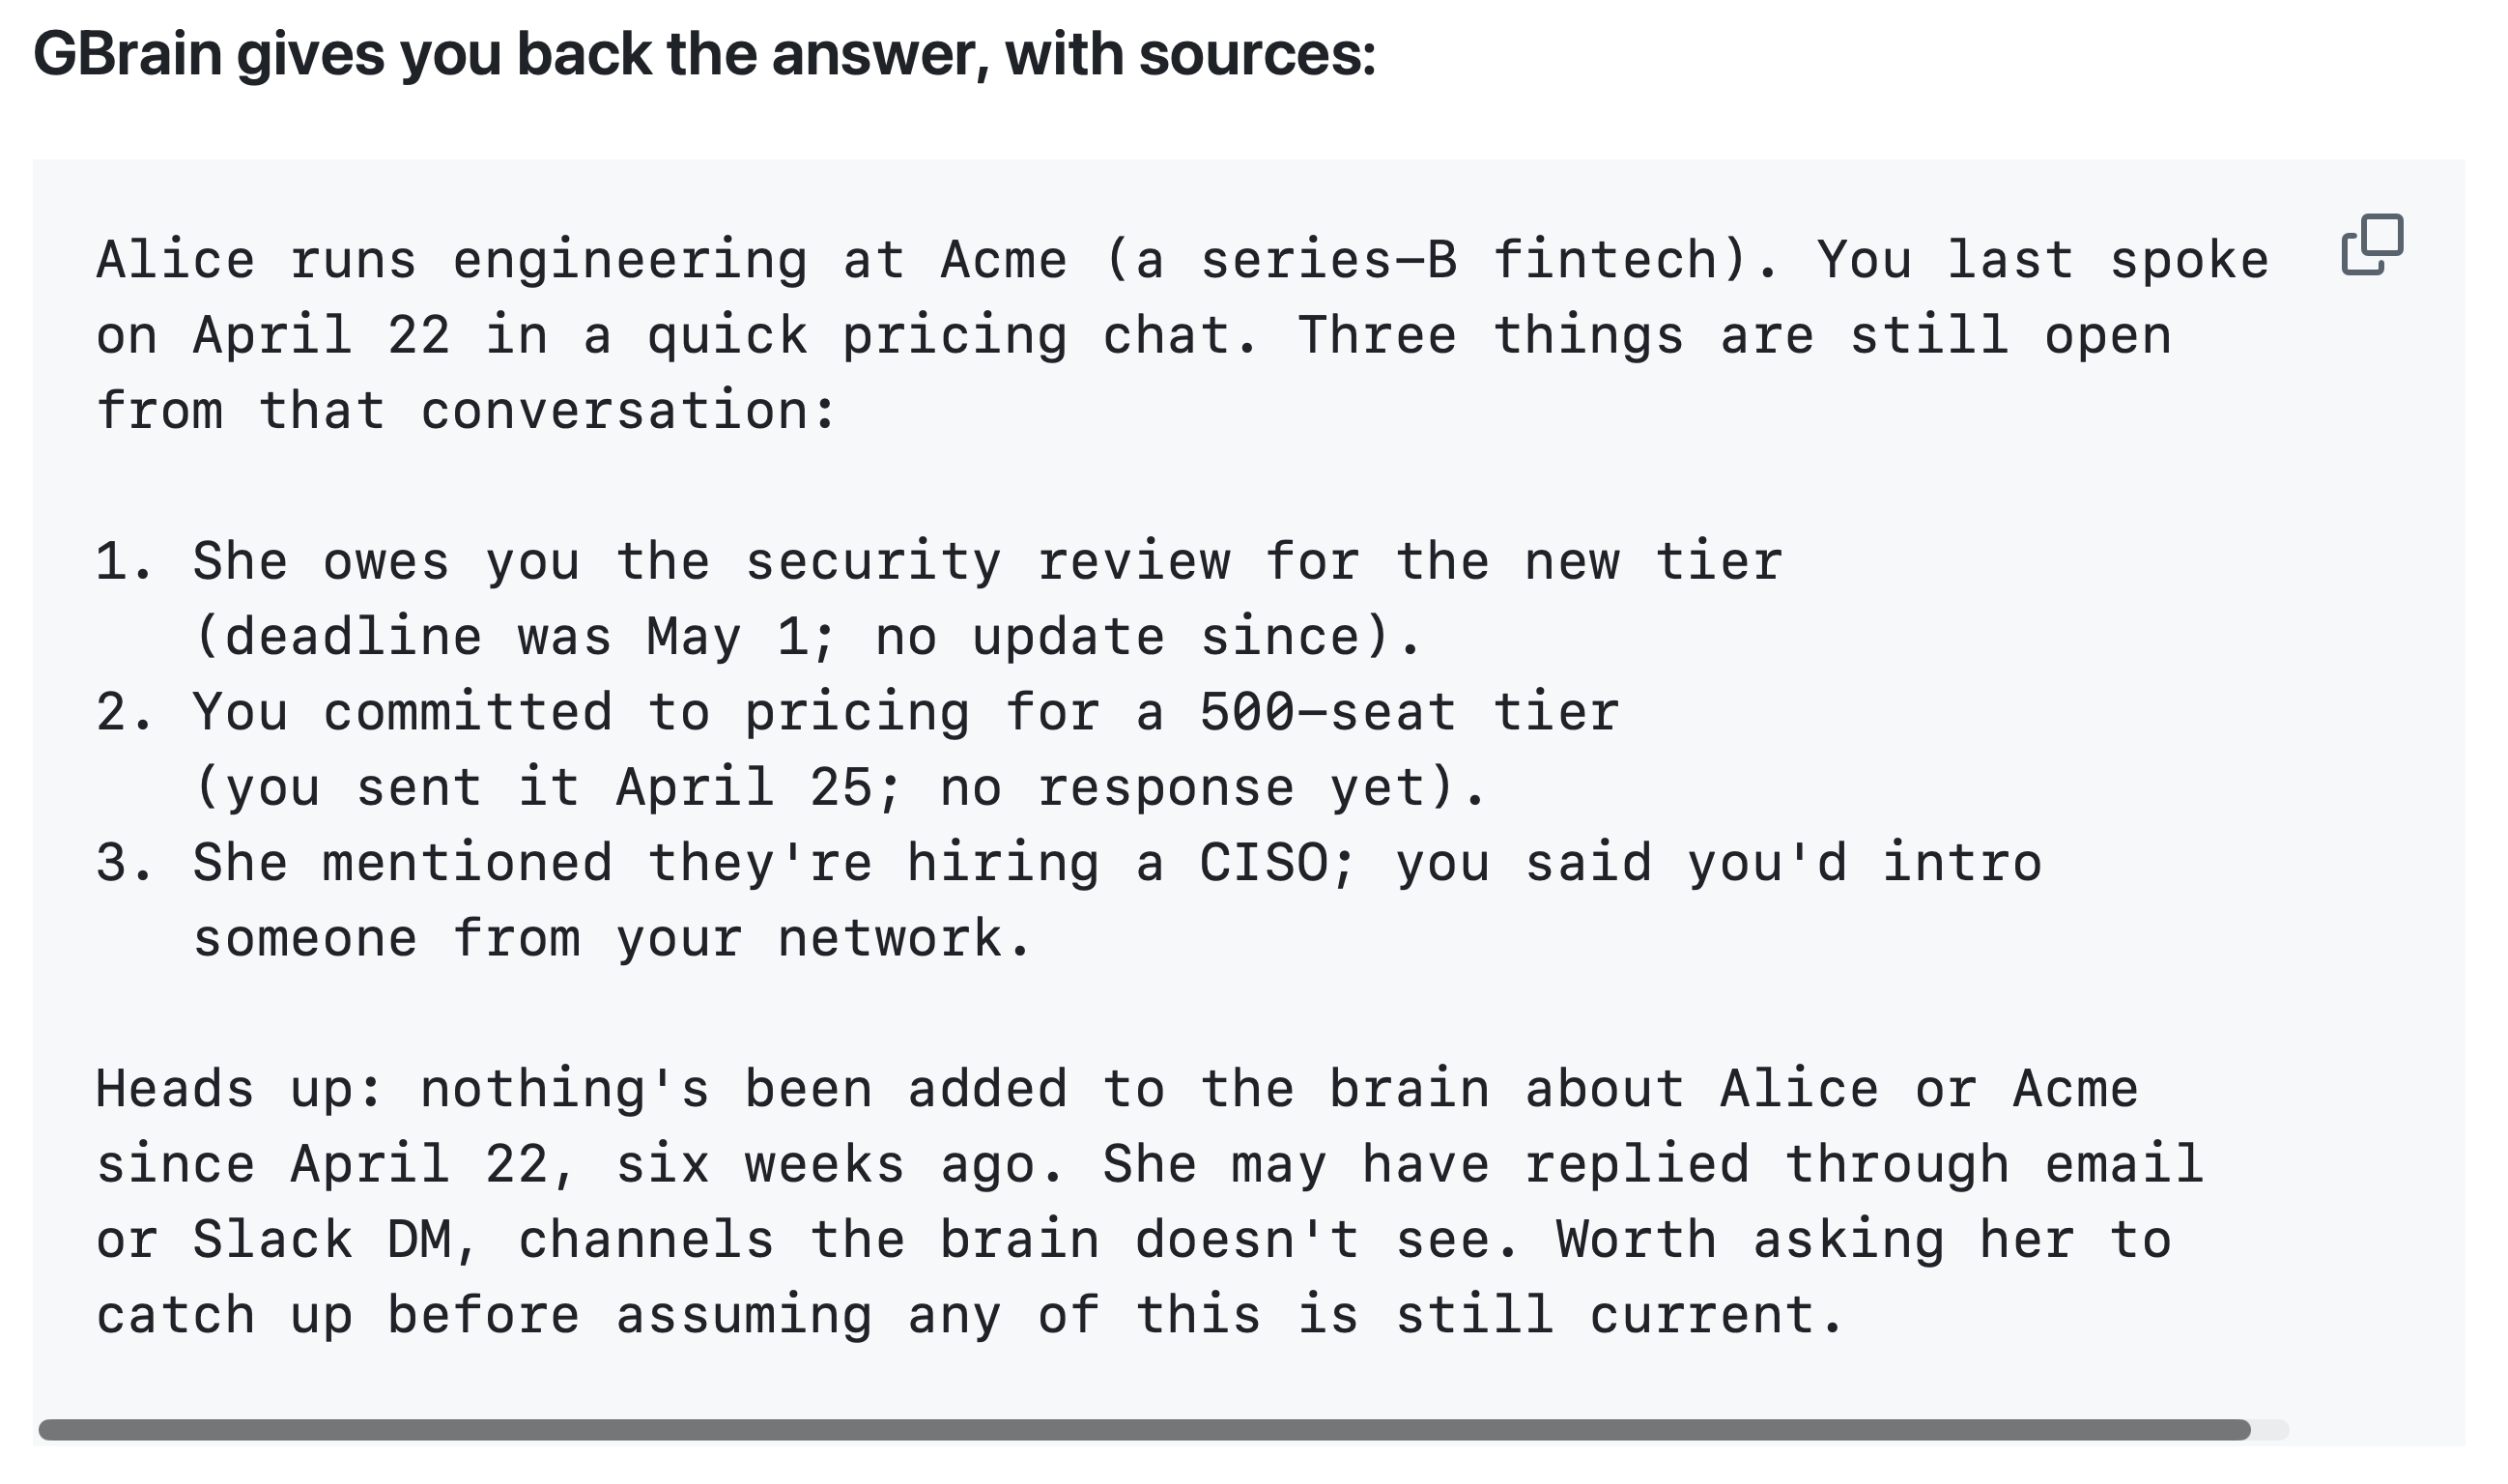
\includegraphics[width=\textwidth]{gbrain3.png}
\end{column}
\begin{column}{0.5\textwidth}
\vs
\begin{itemize}
    \item \ybb{GBrain} indexes a corpus you own -- meeting notes, summaries, Notion --
        and exposes it to the agent as a tool it can query.
    \item The key idea: it (1) searches the corpus, (2) reads the hits for you, and (3) writes the answer.
    \item {\small \yb{\url{github.com/garrytan/gbrain}}}
\end{itemize}
\end{column}
\end{columns}
\end{frame}

% NanoClaw: an agent you reach rather than launch.
\begin{frame}{An agent with an address}
\begin{columns}[T]
\begin{column}{0.5\textwidth}
\begin{center}

\includegraphics[height=0.75\textheight]{nanoclaw.png}
\end{center}
\end{column}
\begin{column}{0.5\textwidth}
\begin{itemize}
    \item \ybb{NanoClaw}: Claude in a Linux container, reached from \yb{WhatsApp,
    Slack, Telegram or email}.
    \item Every minute so far had you at a terminal, driving. Same tool -- reached
    by sending it a message.
    \item A personal-scale project: one process and a handful of files, running in a Linux container.
    \item {\small\yb{\url{github.com/nanocoai/nanoclaw}}}
\end{itemize}
\end{column}
\end{columns}
\end{frame}

% Where to go next, and the repo link.
\begin{frame}{Where to go next}
\begin{itemize}
    \item Try to use it in your own projects and daily life \yob{as much as possible}. 
    \item Brainstorm your ideas, and then \yob{build them}.
\end{itemize}

Other useful resources:
\begin{itemize}
    \item \yb{Agent Skills with Anthropic} -- DeepLearning.AI short course
    \item \yb{Finance skill plugins} by Anthropic 
    \item A collection of resources on AI tools: \yb{\url{www.xuganchen.com/public-goods}}
    \item Alternatively, ask AI to build it for you.
\end{itemize}

\vs
Course materials and every prompt run today:\\ \yb{\url{github.com/xuganchen/BootCamp-Introduction-to-Claude-Code}}

\end{frame}


\end{document}
